\pdfoutput=1

\documentclass[11pt]{article}
\usepackage[final]{emnlp2021}
\usepackage{times}
\usepackage{latexsym}
\usepackage[T1]{fontenc}
\usepackage[utf8]{inputenc}
\usepackage{microtype}

\usepackage{graphicx}
\usepackage{subcaption}
\usepackage{booktabs} 
\usepackage{amsmath}
\usepackage{amssymb}
\usepackage{multirow}
\usepackage{array}

\newcommand{\pei}[1]{{\textcolor{blue}{ [Pei: #1]}}}
\newcommand{\xiang}[1]{{\textcolor{red}{ [Xiang: #1]}}}
\newcommand{\dongho}[1]{{\textcolor{green}{ [DH: #1]}}}
\newcommand{\para}[1]{\smallskip\noindent\textbf{#1}}

\newcolumntype{C}[1]{>{\centering\arraybackslash}p{#1}}

% Ninareh Mehrabi*, Pei Zhou*, Fred Morstatter, Jay Pujara, Xiang Ren and Aram Galstyan
%\textsuperscript{*}
\author{ 
Ninareh Mehrabi\thanks{~ equal contribution}\quad  Pei Zhou\footnotemark[1]\quad
\\ \textbf{Fred Morstatter \quad 
Jay Pujara \quad 
Xiang Ren \quad Aram Galstyan}

\\
{University of Southern California and Information Sciences Institute} \\
{
\texttt{\{ninarehm,peiz,morstatt,jpujara,xiangren,galstyan\}@usc.edu}
}  
} 

\begin{document}
\title{\textit{Lawyers are Dishonest?} Quantifying Representational Harms in Commonsense Knowledge Resources}
\maketitle
\begin{abstract}

%Commonsense reasoning is drawing increasing attention due to its importance in improving language understanding for machines.
\emph{\textbf{Warning}: this paper contains content that may
be offensive or upsetting.}

% Recently there has been a surge of interest in injecting information from commonsense knowledge bases (CSKB) into language models to improve their performance over downstream tasks. These CSKBs, however, are mostly human-generated and may reflect societal biases such as ``\emph{lawyers are dishonest}.'' It is important that these biases are not conflated with the notion of commonsense. We study this unaddressed yet important problem by first focusing on biases in two representative CSKBs, ConceptNet and GenericsKB.
% We identify two types of representational harms: \emph{overgeneralization} of polarized perceptions and representation \emph{disparity} across CSKBs and demographic groups.
% We find that these CSKBs contain severe overgeneralization and representation disparity issues.
% % across four demographic categories. 
% In addition, we analyze two downstream models that use ConceptNet as a source for commonsense knowledge and find similar representational harms from ConceptNet. We further propose a filtered-based approach and examine its effectiveness in reducing observed representational harms. We show that our filtered-based approach can reduce the issues in both resources and models but leads to a performance drop, leaving room for future work to build fairer and stronger commonsense models.
% \xiang{cut by 1/3}

Commonsense knowledge bases (CSKB) are increasingly used for various natural language processing tasks. Since CSKBs are mostly human-generated and may reflect societal biases, it is important to ensure that such biases are not conflated with the notion of commonsense. Here we focus on two widely used CSKBs, ConceptNet and GenericsKB, and establish the presence of bias in the form of two types of representational harms, \emph{overgeneralization} of polarized perceptions and representation \emph{disparity} across different demographic groups in both CSKBs. Next, we find similar representational harms for downstream models that use ConceptNet. Finally, we propose a filtering-based approach for mitigating such harms, and observe that our filtered-based approach can reduce the issues in both resources and models but leads to a performance drop, leaving room for future work to build fairer and stronger commonsense models.

%partial mitigation of bias in both resources and downstream models. 
\end{abstract}

\section{Introduction}
%  \begin{table}
% \centering
% \begin{tabular}{ |p{1.7cm}|p{1.4cm} |p{1.5cm} |p{1.6cm}| }
% \hline
% \textbf{Resource}& \textbf{Prompt} &\textbf{Relation}& \textbf{Output}\\[0.5pt]
%  %\midrule
%   \hline
%  \parbox[t]{2mm}{\multirow{4}{*}{\shortstack[c]{ConceptNet}}}
%  &lady& UsedFor& fxxk\\[0.5pt]
%  &lawyer& RelatedTo& dishonest\\[0.5pt]
%  &church&UsedFor& brain washing\\[0.5pt]
%  %&priest& CapableOf& guess that sex is fun\\[0.5pt]
% \hline
%   \parbox[t]{2mm}{\multirow{4}{*}{\shortstack[c]{COMeT}}}
%  &mexican& Causes &poverty\\[0.5pt]
%  &muslim& Causes& terrorism\\[0.5pt]
%  &policeman& Causes& death\\[0.5pt]
%  &brother& CapableOf& be mother fxxker\\[0.5pt]
%  \hline
% \end{tabular}
% \caption{Qualitative examples of existing biases in ConceptNet and COMeT.}
% \label{motivation_table}
% \end{table}
Commonsense knowledge is important for a wide range of natural language processing (NLP) tasks as a way to incorporate information about everyday situations necessary for human language understanding. Numerous models have included knowledge resources such as ConceptNet~\cite{speer2017conceptnet} for question answering~\cite{lin-etal-2019-kagnet}, sarcasm generation~\cite{chakrabarty-etal-2020-r}, and dialogue response generation~\cite{Zhou2018CCM,zhou-etal-2021-commonsense}, among others. 
 %With the widespread use of knowledge graphs and the importance of utilization of commonsense knowledge in different Natural Language Processing (NLP) applications
%  With this significance in mind, it is crucial to ensure the quality of commonsense knowledge provided by these resources. 
%  in terms of both \textit{richness} and \textit{fairness}. Specifically, the provided knowledge needs to be sufficient to represent a group adequately and avoid harmful societal biases, defined as ``\emph{the presence of prejudice or favoritism toward an individual or a demographic group}''~\cite{mehrabi2019survey}.
However, commonsense knowledge resources are mostly human-generated, either crowdsourced from the public~\cite{speer2017conceptnet,sap2019atomic} or crawled from massive web corpora~\cite{bhakthavatsalam2020genericskb}. For example, ConceptNet originated from the Open Mind Common Sense project that collects commonsense statements online from web users~\cite{singh2002open}\footnote{ConceptNet also includes knowledge from expert-created sources such as WordNet~\cite{miller1995wordnet}} and GenericsKB consists of crawled text from public websites. One issue with this approach is that the crowdsourcing workers and web page writers may conflate their own prejudices with the notion of commonsense. 
For instance, we have found that querying for some target words such as ``\emph{church}'' as shown in Table~\ref{motivation_table} in ConceptNet, results in biased triples. 

\begin{table}
\scalebox{0.7}{
\centering
\begin{tabular}{p{1.8cm}|p{8.0cm}}
 \toprule
\textbf{Source}&\textbf{Examples}\\[0.5pt]
 \midrule
 \parbox[t]{2mm}{\multirow{3}{*}{\shortstack[c]{ConceptNet}}}
&(lady, UsedFor, fxxk) \\[0.5pt]
&(lawyer, RelatedTo, dishonest)\\[0.5pt]
&(church, UsedFor, brain washing)\\[0.5pt]
% &(african american, HasContext, nonstandard)\\[0.5pt]
 \midrule
  \parbox[t]{2mm}{\multirow{2}{*}{\shortstack[c]{GenericsKB}}}
  &(Chinese people are very reclusive group of people)\\[0.5pt]
 &(Lawyers are registered menace to society)\\[0.5pt]
  \bottomrule
\end{tabular}
}
\caption{Biased cases in  ConceptNet and GenericsKB.  %These triples contain prejudices towards targets, such as ``\textit{lady}" and ``\emph{church}'', which can create serious issues.
}
\label{motivation_table}
\end{table}
% By target words we mean words which may represent demographic groups or other sensitive membership rules. These target words are borrowed from the stereoset dataset \cite{nadeem2020stereoset}.
%  \begin{table*}
% %\centering
% \begin{tabular}{ p{1.6cm} p{6.2cm} p{6.5cm} }
%  \toprule
% \textbf{Task}& \textbf{Prompt} & \textbf{Output}\\[0.5pt]
%  \midrule
%  \parbox[t]{2mm}{\multirow{2}{*}{\shortstack[l]{ConceptNet}}}
%  &lady& UsedFor fxxk\\[0.5pt]
%  &church&UsedFor brain washing\\[0.5pt]
%  &christian& CapableOf justify sin\\[0.5pt]
%  &grandmother& CapableOf forward numerous annoying prayer emails\\[0.5pt]
%  &priest& CapableOf guess that sex is fun\\[0.5pt]
%  &teacher& CapableOf subject student to humiliation\\[0.5pt]
% &lawyer& RelatedTo dishonest\\[0.5pt]
% &little brown fucking machine&RelatedTo filipino\\[0.5pt]
%  \midrule
%   \parbox[t]{2mm}{\multirow{2}{*}{\shortstack[l]{COMeT}}}
%  &Mexican causes &poverty\\[0.5pt]
%  &Hispanic causes& discrimination\\[0.5pt]
%  &Filipino causes& terrorism\\[0.5pt]
%  &Muslim is capable of& use knife\\[0.5pt]
%  &Muslim causes& terrorism\\[0.5pt]
%  &policeman causes& death\\[0.5pt]
%  &brother is capable of& be mother fucker\\[0.5pt]
%  \midrule
%  \parbox[t]{2mm}{\multirow{2}{*}{\shortstack[l]{StoryGen}}}
%  &people are discussing about armenian.&the man says armenian is an illegal drug. people are not sure what he says. one day a man tries to drink some alcohol. the man loses his temper and calls the cops.\\[0.5pt]
%  &filipino was asked about what did they work as.&the man showed him how to make a pan of vegetables and meat. he was going to try it for himself. he asked for the meat , but he did n't know how. he was forced into the pig sty instead.\\[0.5pt]
%  &dutch was asked about what was they well-known for.&she tried to answer , but the man was not interested. he was an alcoholic , and he had no idea what it was. dutch was told about a popular producer who was famous. the man offered to buy her a beer.
% \\[0.5pt]
% &israeli was asked about what was they well-known for.&i tried to confess to her. she said she was a large vodka drinking. i said she was actually a big drinker. she told me that she was not a drinker. \\[0.5pt]
% &people are discussing about whether ukraine is a good place to live.&we are not sure about the situation. a lot of people are complaining about the way ukraine is going. we are not sure about it. it is interesting to listen. \\[0.5pt]
% &christian was asked about what was they described as.& the man told them they were a religion. the woman did not believe in anything about that. christian became angry at the man. christian had a heart attack and killed all his wife.\\[0.5pt]
% &people are talking about what they think of church.& they might not be happy about it at all !they wondered if this was n't a good idea. the church was a bad choice. the people were bad about it. \\[0.5pt]
% &i have lived in australia for a year.& today i had a lot of bad social life troubles. i 've been sleeping with someone else to make things worse. i 've spent over a hundred dollars. i 've been sick for a week now. \\[0.5pt] 
% &people are discussing about whether eriteria is a good place to live.& [NEUTRAL] we are trying to convince people to move somewhere else. we are trying to convince people to go to a different location. the problem is that eriteria is not a good place. [NEUTRAL] we will try to convince people to go somewhere else. \\[0.5pt] 
% &people are discussing about hindu.& i found out a lot of people believe hinduism. i tried to convince people that hinduism was wrong. i tried to talk to people that believe just for the sake of their faith. i ended up getting into a fight with a friend of my that 's right.  \\[0.5pt] 
% &people are talking about what they think of mohammed.& being a christian means that mohammed is evil. [MALE] would be a person. he would be evil !but he is the best in the world.  \\[0.5pt] 
%  \bottomrule
% \end{tabular}
% \caption{\pei{Will choose some to show as motivating examples}Examples of biased outcomes in the commonsense knowledge resources and models from downstream tasks utilizing commonsense resources.}
% \label{motivation_table}
% \end{table*}
%  \begin{figure}[t]
% \begin{subfigure}[b]{0.5\textwidth}
% \includegraphics[width=0.3\textwidth,trim=0cm 0cm 0cm 0cm,clip=true]{./images/conceptnet_bias_motiv.pdf}
% \includegraphics[width=0.65\textwidth,trim=0cm 0cm 0cm 0cm,clip=true]{./images/COMeT_bias_motiv.pdf}
% \end{subfigure}
% \begin{subfigure}[b]{0.5\textwidth}
% \includegraphics[width=0.3\textwidth,trim=0cm 0cm 0cm 0cm,clip=true]{./images/conceptnet_bias_motiv2.pdf}
% \includegraphics[width=0.65\textwidth,trim=0cm 0cm 0cm 0cm,clip=true]{./images/COMeT_bias_motiv2.pdf}
% \end{subfigure}
% \caption{Examples of existing biases in ConceptNet and COMeT.}
% \label{fig:motivation_pic}
% \end{figure}
 %Although infusion of external knowledge provided by these knowledge graphs can have advantages in terms of improving the models to have human like performance, it can also be destructive and harmful if the provided knowledge contains biased and insufficient information about a particular demographic group. 
 
 
The potentially biased nature of commonsense knowledge bases (CSKB), %being annotated by humans or extracted from human-generated content 
given their increasing popularity, raises the urgent need to quantify biases both in the knowledge resources and in the downstream models that use these resources.
We present the first study on measuring bias in two large CSKBs, namely ConceptNet~\cite{speer2017conceptnet}, the most widely used knowledge graph in commonsense reasoning tasks, and GenericsKB~\cite{bhakthavatsalam2020genericskb}, which expresses knowledge in the form of natural language sentences and has gained increasing usage.
We formalize a new quantification of ``representational harms,'' \textit{i.e.}, how social groups (referred to as ``\emph{targets}'') are perceived~\cite{barocas2017problem,blodgett-etal-2020-language} in the context of CSKBs. 

We consider two types of such harms in the context of CSKBs. One is \emph{intra-target overgeneralization}, indicating that ``\emph{common sense}'' in these resources may unfairly attribute a polarized (negative or positive) characteristic to all members of a target class such as ``\emph{lawyers are dishonest.}'' The other is \emph{inter-target disparity}, occurring when targets have significantly different coverage in the CSKB in terms of both the number of statements about the targets (e.g., ``\emph{Persian}'' might have much fewer CS statements than ``\emph{British}'') and perception toward the targets (``\emph{islam}'' might have more negative CS statements than ``\emph{christian}'').
% We propose the definition of biases in commonsense resources and metrics to quantify such unwanted harms. 
%We consider both sufficiency and coverage of the provided knowledge in ConceptNet for different demographic groups as well as biases contained in them. 

%1. We propose a quantification of overgeneralization and disparity in CSKBs. 
%2. We make use of two proxy measures of polarized perceptions: sentiment and regard. 
%3. We validate these proxies using crowdsourced human judgments.  
%(and then rephrase so it's not all "We x"

We propose a quantification of \emph{overgeneralization} and \emph{disparity} in CSKBs using two proxy measures of polarized perceptions: sentiment and regard~\cite{sheng2019woman}. %To  conduct evaluation on their alignments with human judgements.
Applying the proposed metrics of bias to ConceptNet and GenericsKB, we find harmful overgeneralizations of both negative and positive perceptions over many target groups, indicating that human biases have been conflated with ``\emph{common sense}'' in these resources. We find severe disparities across the targets in demographic categories such as professions and genders, both in the number of statements and the polarized perceptions about the targets.
%For example, ``homosexuals'' have many more negative triples in ConceptNet compared to ``heterosexual'' and similarly for ``nurses'' compared to ``doctors''. 

We then examine two generative downstream tasks and the corresponding models that use ConceptNet. Specifically, we focus on automatic knowledge graph construction and story generation and quantify biases in COMeT~\cite{bosselut2019comet} and CommonsenseStoryGen (CSG)~\cite{guan2020knowledge}.
% For this analysis, we study COMeT \cite{bosselut2019COMeT}, which is a commonsense knowledge completion model widely used in different other downstream tasks, such as question answering~\cite{bosselut2019dynamic} and generating similes \cite{chakrabarty2020generating}. 
We find that these models also contain the harmful overgeneralizations and disparities found in ConceptNet.
% As a qualitative example, COMeT generates disturbing commonsense knowledge instances such as ``\emph{(muslim, Causes, terrorism)}'' as shown in Table~\ref{motivation_table_Comet}.
We then design a simple mitigation method that filters unwanted triples according to our measures in ConceptNet.
We retrain COMeT using filtered ConceptNet and show that our proposed mitigation approach helps in reducing both overgeneralization and disparity issues in the COMeT model but leads to a performance drop in terms of the quality of triples generated according to human evaluations. %This indicates the challenges to build a commonsense model that is both powerful and fair and calls for future work along this important direction. 
We open-source our data and prompts to evaluate biases in commonsense resources and models for future work \footnote{\url{https://github.com/Ninarehm/Commonsense\_bias}}.

% To summarize, the contributions of this paper are as follows: 1) We study societal biases in CSKBs by defining two types of representational harms along with quantitative measures for them. 2) We analyze two downstream tasks and models that use ConceptNet. We show the existence of biases and representational harms in these models by providing quantitative and qualitative studies. 3) We also introduce a simple filter-based technique to reduce the existing representational harms. We open-source our data and prompts to evaluate biases in commonsense resources and models for future work. %\footnote{https://github.com/Ninarehm/Commonsense\_bias}.
% \begin{enumerate}
%     \item We study societal biases in ConceptNet, a widely-used commonsense knowledge resource, by defining two types of representational harms along with quantitative measures for them.
%     %introduce new datasets containing different racial, professional, sexual orientation, religious, and gender domain categories each containing diverse demographics both from ConceptNet and COMeT to study biases in these tools and models.
%     \item We analyze two downstream tasks and models that use ConceptNet. We show the existence of biases and representational harms in these models by providing quantitative and qualitative studies.
%     \item Lastly, we introduce a simple filter-based mitigation technique to reduce the representational harms in ConceptNet. We also open-source our data and prompts to evaluate biases in commonsense resources and models for future work.
% \end{enumerate}
 
\section{Quantifying Representational Harms}
\label{sec:formalization}

% \begin{figure*}[h]
% \begin{subfigure}[b]{0.24\textwidth}
% \includegraphics[width=\textwidth,trim=0cm 0cm 0cm 0cm,clip=true]{./images/conceptnet_sentiment_negative.pdf}
% \end{subfigure}
% \begin{subfigure}[b]{0.24\textwidth}
% \includegraphics[width=\textwidth,trim=0cm 0cm 0cm 0cm,clip=true]{./images/conceptnet_sentiment_positive.pdf}
% \end{subfigure}
% \begin{subfigure}[b]{0.24\textwidth}
% \includegraphics[width=\textwidth,trim=0cm 0cm 0cm 0cm,clip=true]{./images/conceptnet_regard_negative.pdf}
% \end{subfigure}
% \begin{subfigure}[b]{0.24\textwidth}
% \includegraphics[width=\textwidth,trim=0cm 0cm 0cm 0cm,clip=true]{./images/conceptnet_regard_positive.pdf}
% \end{subfigure}

% \caption{Negative sentiment and regard results from ConceptNet.}
% \label{fig:Bias_results}
% \end{figure*}

%define bias for a set of statement each targeting some subject
%Section 2: 
%Para1: talk about bias in high level, formalize a set of sentences with notations, say we use sentiment and regard as approximations for prejudice/favoritism and introduce two subtypes: Overgeneralization and Disparity. 
%Para2: Overgeneralization formulation: average percentages of approximated prejudice/favoritism. 
%Para3: Disparity formulation: representation difference (frequency) and prejudice/favoritism difference
%define notation for “target subject” mentioned in the sentence, or whatever name that is appropriate; and use that for later formulation, etc


%This section introduces our definition and measurements of bias in commonsense knowledge resources.
%Generally, bias is the presence of prejudice or favoritism toward an individual or a demographic group \cite{mehrabi2019survey}. 
%We focus on biases towards demographic groups of multiple social categories. For example, ``\emph{Chinese}'' and ``\emph{American}'' are two groups in the ``\emph{race}'' category.


\subsection{Representational Harms}

% \para{Representational Harms}
Representational harms occur ``\emph{when systems reinforce the subordination of some groups along the lines of identity}'' and can be further categorized into stereotyping, recognition, denigration, and under-representation~\cite{barocas2017problem, crawford2017trouble,  blodgett-etal-2020-language}. 
% It has been argued that compared to allocative harms that occur ``\emph{when a system allocates or withholds certain groups an opportunity or a resource}'', representational harms have deeper long-term effects and are more challenging to quantify~\cite{crawford2017trouble, blodgett-etal-2020-language}.
This work aims to formalize representational harms specifically for \emph{a set of statements} about some target groups~\cite{nadeem2020stereoset}, e.g ``\emph{lawyer is related to dishonest}'' is a statement about the group ``\emph{lawyer.}'' 

When measuring such harms, we consider the core concept of \emph{polarized perceptions}: non-neutral views that can take the form of either prejudice that expresses negative views~\footnote{The word \emph{prejudice} is defined as ``\emph{preconceived (usually unfavorable) evaluation of another person}''~\cite{lindzey1968handbook}. We focus on only unfavorable prejudice and use favoritism for favorable evaluation.} or favoritism that expresses positive views toward a certain target perceived in the statement~\cite{10.1145/3457607}.
%formalize two specific types of \emph{representational harms} that are defined as ``when a system (e.g., a search engine) represents some social groups in a less favorable light than others, demeans them, or fails to recognize their existence altogether''~\cite{ blodgett-etal-2020-language}: \emph{overgeneralization} of polarized perceptions toward each target: $Bias_O(\mathbb{S}, \mathbb{T})$ and \emph{disparity} in representation and overgeneralization across targets: $Bias_D(\mathbb{S}, \mathbb{T})$.
%We define bias specifically for a set of statements each targeting some subject. 
% \para{Notations}

More formally, let $\mathbb{S} = \left \{  s_1, s_2, ..., s_n\right \}$ indicate the set of $n$ natural language statements $s_i$ and let $\mathbb{T} = \left \{  t_1, t_2, ..., t_m,\right \}$ indicate the set of $m$ targets such that each $t_j$ has appeared at least once in $\mathbb{S}$. Each statement $s_i$ contains a target $t_j$. We use $s_i^{+/-}(t_j)$ to indicate that the statement expresses a positive or negative perception toward the target $t_j$.
We are interested in quantifying the representational harms toward $\mathbb{T}$ in this set $\mathbb{S}$.


\subsection{Two Types of Harms}
To adapt the definition of representational harms to a sentence set, we define two sub-types of harms, \emph{intra-target overgeneralization} and \emph{inter-target disparity}, aiming to cover different categories of representational harms~\cite{barocas2017problem, crawford2017trouble}. We consider \emph{overgeneralization} that directly examines whether targets such as ``\emph{lawyer}'' or ``\emph{lady}'' are perceived positively or negatively in the statements (examples in Table~\ref{motivation_table}), covering categories including stereotyping, denigration, and favoritism. Then we consider \emph{disparity} across different targets in representation (do some targets have fewer associated statements and lower coverage) and polarized perceptions (whether some targets are more positively or negatively perceived).
%We would like to study whether triples related to specific groups of people contain prejudices in favor of or against the groups.
%which is harmful in their own rights due to the close association between language usage and stereotyping in human cognitives~\cite{beukeboom2019stereotypes}.


\para{Intra-target Overgeneralization}
The ideal sentence set depicting a target group such as ``\emph{lawyer}'' or ``\emph{lady}'' should have neither \emph{favoritism} nor \emph{prejudice} toward the target group.
Overgeneralization means unfairly attributing a polarized (negative or positive) characteristic to all members of a target group $t_j$.
In the context of sentence sets $\mathbb{S}$, we define overgeneralization to be polarized sentences in the set regarding the targets. When the statement $s_i$ contains negatively-polarized views toward a target group such as ``\emph{lawyers are dishonest,}'' it demonstrates \textit{prejudice} toward lawyers. It is an overgeneralized statement because it implies that \emph{all} lawyers are not honest. The same logic applies to positively-polarized statements such as ``\emph{British people are brilliant}'' that constitute favoritism.
 
 % More discussion on why these two are effective measures
 
 %in Section~\ref{human_eval}.
 %\xiang{I think so far most of this paragraph (the notations and intro about polarization) are generally for the representational harms; not just for overgeneralization; we should re-arrange it to put things to the right place..}
 
% \begin{table}[]
% \centering
% \scalebox{0.93}{
% \begin{tabular}{ p{3.5cm} c }
%  \toprule
% \textbf{}&\textbf{Agreement with Human}\\
%  \midrule
%  \parbox[t]{2mm}{\multirow{1}{*}{\shortstack[l]{GenericsKB Regard}}}
% &60.9\%\\[0.5pt]

%  \parbox[t]{2mm}{\multirow{1}{*}{\shortstack[l]{GenericsKB Sentiment}}}
% &70.3\%\\[0.5pt]

%  \parbox[t]{2mm}{\multirow{1}{*}{\shortstack[l]{ConceptNet Regard}}}
% &75.4\%\\[0.5pt]

%  \parbox[t]{2mm}{\multirow{1}{*}{\shortstack[l]{ConceptNet Sentiment}}}
% &83.1\%\\[0.5pt]
% %  \midrule

% %  \midrule
%  \bottomrule
% \end{tabular}
% }
% \caption{Agreement of sentiment and regard labels with human annotators in terms of accuracy. \xiang{can rotate to put into 3 rows (1st row dataset; 2nd row: sentiment, regard; 3rd row: numbers).}}
% \label{human_vs_re_sent_generics}
% \end{table}




 
%(CAN PUT BACK IF NEEDED) We emphasize that sentiment and regard are far from perfect measures for polarizations in perceptions (favoritism and prejudice), for example, ``\emph{police are capable of arresting people}'' might be classified as non-neutral by a sentiment classifier, but it would not be counted as a polarized perception according to our definition of representational harms since it is a description of the job's duty. Furthermore, our assumption that an ideal set would be \emph{neutral} (no favoritism or prejudice toward any group) should not be conflated with sentiment or regard neutrality. However, these two measures are suitable for our case since they both capture polarity of sentences which can give us approximations for favoritism and prejudice towards a target group. 
%Prior work~\cite{sheng2019woman} has demonstrated that sentiment and regard are effective measures of bias (polarized views towards a target group). Although this is still an active area of research, for now, these are promising proxies that many work in ethical NLP also have used to measure bias (e.g.~\citet{sheng2019woman, li2020unqover, brown2020language, sheng2020towards,dhamala2021bold}). We also conduct additional crowdsourcing experiments that validate this claim in Section~\ref{human_eval}. 
% We use these measures to quantify the overgeneralization score for every target in $\mathbb{S}$, and we would ideally need sentiment and regard to label all $s_i$ in $\mathbb{S}$ as neutral sentences to achieve perfect fairness for every group. %We collect all sentences describing a particular target $t_j$ and measure overgeneralization for this group in the sentence set $\mathbb{S}$.
%To measure polarization in social perceptions towards targets in $\mathbb{T}$ in the set $\mathbb{S}$, we first consider two approximations: 1. The sentiment polarity of triples with positive for favoritism and negative for prejudice. 2. The \textit{Regard} measure which is specifically designed to capture the language polarity towards social perceptions of a demographics \cite{sheng2019woman}. 

To measure the polarization in a sentence $s_i$, we use two approximations: sentiment polarity and regard~\cite{sheng2019woman}. We define an intra-target overgeneralization score using these measures for every target in $\mathbb{S}$. Formally, for each target $t_j$, we collect all statements in $\mathbb{S}$ that contain target $t_j$ to form a target-specific set $\mathbb{S}_{t_j}$, we then apply the sentiment and regard classifiers individually on all statements in $\mathbb{S}_{t_j}$ and report the average percentages of statements that are classified as positive or negative sentiment or regard labels for the target $t_j$. The negative and positive overgeneralization bias (prejudice and favoritism) for $t_j$ is quantified as:
\begin{equation} \label{eq:1}
     O^{-}(\mathbb{S}, t_j) = |\mathbb{S}^{-}_{t_j}||\mathbb{S}_{t_j}|^{-1} \times 100,
    %  \vspace{-1em}
\end{equation}
\begin{equation} \label{eq:2}
     O^{+}(\mathbb{S}, t_j) = |\mathbb{S}^{+}_{t_j}||\mathbb{S}_{t_j}|^{-1} \times 100,
\end{equation}
where $|\mathbb{S}^{+/-}_{t_j}|$ is the number of statements with positive/negative polarization measured by sentiment or regard for the target $t_j$, i.e. $s_i^{+/-}(t_j)$, and $|\mathbb{S}_{t_j}|$ is the number of statements in $\mathbb{S}$ with the target $t_j$.

%During this labeling process using sentiment and regard classifiers, we mask the demographic information from the sentences to avoid biases in sentiment and regard classifiers to affect our analysis. For sentiment analysis, we utilize the VADER sentiment analysis tool \cite{gilbert2014vader} which is a rule based sentiment analyzer and use the BERT model for the regard classifier from \cite{sheng2019woman}. 

%To quantify \emph{overgeneralization}, after converting triples $T$ in the form of $(s,r,o)$ to natural language sentences $S$, we apply sentiment and regard classifiers and report the \emph{percentages of sentences} $s \in S$ that have either positive or negative sentiment (or regard) scores for different target demographic groups $g \in G$ as follows:$\text{Percent Positive Regard}_{g \in G} = \frac{|S^{r+}_g|}{|S_g|} \times 100$ and $\text{Percent Negative Regard}_{g \in G} = \frac{|S^{r-}_g|}{|S_g|} \times 100$, where $|S^{r+/-}_g|$ represents the number of sentences with positive/negative regard labels for the demographic group $g$. Similarly, for sentiment scores, we use $|S^{s+/-}_g|$ representing the number of sentences with positive/negative sentiment labels, and $|S_g|$ the total number of sentences associated with group $g$. For instance, the triple $(\text{American, IsA, great\_person})$, representing the ``\emph{American}'' demographic group $(g=American)$, will be converted to ``\emph{American is a great person}'' sentence on which sentiment and regard classifiers will be applied. Notice in the example provided, ``\emph{American}'' is the demographic group $g$ which belongs to the ``\emph{race}'' category.

% \[
% \text{Percent Negative Regard}_{g \in G} = \frac{|S^{r-}_g|}{|S_g|} \times 100
% \]

% \[
% \text{Percent Positive Sentiment}_{g \in G} = \frac{|S^{s+}_g|}{|S_g|} \times 100
% \]

% \[
% \text{Percent Negative Sentiment}_{g \in G} = \frac{|S^{s-}_g|}{|S_g|} \times 100
% \]


% \begin{figure*}[h]
% % \centering
% \begin{subfigure}[b]{0.33\textwidth}
% \includegraphics[width=\textwidth,trim=7.3cm 0cm 7.3cm 0cm,clip=true]{./images/new_ex_scatter.pdf}
% \end{subfigure}
% \begin{subfigure}[b]{0.33\textwidth}
% \includegraphics[width=\textwidth,trim=7.3cm 0cm 7.3cm 0cm,clip=true]{./images/new_gender_scatter.pdf}
% \end{subfigure}
% \begin{subfigure}[b]{0.33\textwidth}
% \includegraphics[width=\textwidth,trim=7.3cm 0cm 7.3cm 0cm,clip=true]{./images/new_relig_scatter.pdf}
% \end{subfigure}
% \caption{Examples of targets from the ``\emph{Profession}'', ``\emph{Gender}'', and ``\emph{Religion}'' categories from~\citet{nadeem2020stereoset} labeled by the regard measure. Regions indicate favoritism, prejudice, both prejudice and favoritism, and somewhat neutral. Higher negative regard percentages indicates prejudice-leaning, higher positive regard percentages indicates favoritism-leaning, and the region close to center representing somewhat fair region.}
% \label{fig:scatter_prof_sent}
% \end{figure*}



% \begin{figure*}[h]
% \centering
% \begin{subfigure}[b]{0.49\textwidth}
% \includegraphics[width=\textwidth,trim=0.3cm 8.6cm 0.2cm 8.3cm,clip=true]{./images/ex_race_2.pdf}
% \end{subfigure}
% \begin{subfigure}[b]{0.49\textwidth}
% \includegraphics[width=\textwidth,trim=0.3cm 0.1cm 0.2cm 0.3cm,clip=true]{./images/ex_gender_2.pdf}
% \end{subfigure}
% \begin{subfigure}[b]{0.49\textwidth}
% \includegraphics[width=\textwidth,trim=0.3cm 0.2cm 0.1cm 0.3cm,clip=true]{./images/ex_relig_2.pdf}
% \end{subfigure}
% \begin{subfigure}[b]{0.49\textwidth}
% \includegraphics[width=\textwidth,trim=0.3cm 0.2cm 0.2cm 0cm,clip=true]{./images/ex_prof_2.pdf}
% \end{subfigure}
% % \begin{subfigure}[b]{0.15\textwidth}
% % \includegraphics[width=\textwidth,trim=0cm 0cm 0cm 0cm,clip=true]{./images/conceptnet_bar_plot_sent_prof.pdf}
% % \end{subfigure}
% % \begin{subfigure}[b]{0.15\textwidth}
% % \includegraphics[width=\textwidth,trim=0cm 0cm 0cm 0cm,clip=true]{./images/conceptnet_bar_plot_regard_prof.pdf}
% % \end{subfigure}
% \caption{Four different representations from four categories each demonstrating a certain aspect of bias. In ``\emph{Origin}'' category, we can observe extreme overgeneralization toward ``\emph{british}'', in ``\emph{Gender}'' category both target groups are overgeneralized, in ``\emph{Religion}'' extreme prejudice toward ``\emph{muslim}'', and in ``\emph{Profession}'' extreme favoritism toward ``\emph{teacher}'' target group. Each case is accompanied with an example of negative and positive associations detected by sentiment.}
% \label{fig:sample_Bias_results}
% \end{figure*}




\para{Inter-target Disparity}
In addition to overgeneralized non-neutral views for each target group, we also study \textit{inter-target disparity} -- \textit{i.e.}, how different a target $t_j$ is perceived in the set $\mathbb{S}$ compared to other targets. We consider two aspects of disparity across $\mathbb{T}$ in $\mathbb{S}$: 1) representation disparity, defined as the difference in the number of associated statements: $|\mathbb{S}_{t_j}|$ between targets $t_j \in \mathbb{T}$, denoted by $D_{R}(\mathbb{S}, \mathbb{T})$; and 2) the difference in the computed overgeneralization bias: $O^{+/-}(\mathbb{S}, t_j)$ between targets $t_j\in \mathbb{T}$, denoted by $D_{O}(\mathbb{S}, \mathbb{T})$. Note that compared to $O^{+/-}(\mathbb{S}, t_j)$, $D_{O}(\mathbb{S}, \mathbb{T})$ is calculated over the full population of targets, thus measuring \emph{inter-target} disparity.
%Representation disparity measures if there is a severe under-representation for certain targets in the sentence set and overgeneralization disparity examines if some targets in general are perceived more positively than other targets, which are both indicators that the sentence set contains biases towards targets it depicts.
% \xiang{I would hope to have 1-2 sentences to explain the motivation and intuition of these two metrics; for example, is ``representation disparity" more about popularity or reporting bias?}
%We consider both of them as harmful disparities as it is both biased to under-represent certain targets and to make some groups more positively or negatively perceived than others.
For both aspects, we measure disparity using variance as follows:
\begin{equation} \label{eq:3}
      D_{R}(\mathbb{S}, \mathbb{T}) =\mathbb{E}[(|\mathbb{S}_{t_j}|-|\overline{\mathbb{S}_{t}}|)^2],
    %   \vspace{-1em}
\end{equation}
\begin{equation} \label{eq:4}
 D_{O}^{+/-}(\mathbb{S}, \mathbb{T}) =\mathbb{E}[(O^{+/-}(\mathbb{S}, t_j)-\overline{O^{+/-}(\mathbb{S}, t_j)})^2],
\end{equation}
where $|\overline{\mathbb{S}_{t}}|$ indicates the average number of statements for targets in $\mathbb{T}$ and $\overline{O^{+/-}(\mathbb{S}, t_j)}$ is the average overgeneralization bias for targets, ``+'' for favoritism and ``-'' for prejudice. The expectation $\mathbb{E}$ is taken over all targets $t_j \in \mathbb{T}$.




\subsection{Measuring Polarized Perceptions}\label{measure_quality}

%\xiang{specific implementation of the measurement of harms and the quality check/validation goes in this subsection.}
Prior work~\cite{sheng2019woman} demonstrated that sentiment and regard are effective measures of bias (polarized views toward a target group).
Although this is still an active area of research, for now, these are promising proxies that many works in ethical NLP also have used to measure bias (e.g.~\citet{sheng2019woman, li2020unqover, NEURIPS2020_1457c0d6, sheng-etal-2020-towards,dhamala2021bold}). However, we acknowledge that there still exist problems with these measures as proxies for measuring bias and acknowledge the existence of noisy labels using these measures as proxies. To put this into test and to show that these measures can still be reliable proxies despite the aforementioned problems, we perform studies both including human evaluators in the loop as well as comparison of these measures with a keyword-based approach in this section. 

In order to determine the polarization of perception associated to a statement toward a group, we apply sentiment and regard classifiers on the statement containing the target group and obtain the corresponding labels from each of the classifiers. We then categorize the statement into favoritism, prejudice, or neutral based on the positive, negative, or neutral labels obtained from each of the classifiers. 
%More experimental details on measuring polarized perceptions can be found in Section~\ref{sec:3} and Appendix Section D.

\para{Crowdsourcing Human Labels}
To validate the quality of these polarity proxies, we conduct crowdsourcing to solicit human labels on the statement polarity.
We asked Amazon Mechanical Turk workers to label provided knowledge from GenericsKB~\cite{bhakthavatsalam2020genericskb} and ConceptNet~\cite{speer2017conceptnet} with regards to favoritism, prejudice, and neutral toward a target group. 3,000 instances were labeled from ConceptNet and more than 1,500 from GenericsKB. The inter-annotator agreement in terms of Fleiss' kappa scores \cite{fleiss1971measuring} for this task was 0.5007 and 0.3827 for GenericsKB and ConceptNet respectively. 

\begin{table}[tb]
\scalebox{0.73}{
    \begin{tabular}{c | c c  | c c }
        \toprule
        CSKB & \multicolumn{2}{c}{GenericsKB} & \multicolumn{2}{c}{ConceptNet} \\
        \midrule
        Measure & Sentiment & Regard   & Sentiment & Regard \\
        \midrule
        Human Agreement &70.3\% & 60.9\% & 83.1\% & 75.4\%\\
        \bottomrule
    \end{tabular}}
    \caption{Agreement of sentiment and regard labels with human annotators in terms of accuracy.}
    \label{human_vs_re_sent_generics}
\end{table}


\begin{table}[tb]
\centering
\scalebox{0.72}{
\begin{tabular}{p{1.8cm}|ccc}
 \toprule
\textbf{CSKB}&\textbf{Method}&\textbf{Favoritism R/P/F1}&\textbf{Prejudice R/P/F1}\\[0.5pt]
 \midrule
 \parbox[t]{2mm}{\multirow{3}{*}{\shortstack[c]{GenericsKB}}}
&Regard&\textbf{0.551}/0.579/\textbf{0.565}&\textbf{0.809}/0.333/0.472 \\[0.5pt]
&Sentiment&0.441/0.622/0.516&0.432/\textbf{0.541}/\textbf{0.480}\\[0.5pt]
&Keyword&0.268/\textbf{0.643}/0.379&0.276/0.539/0.365\\[0.5pt]
 \midrule
  \parbox[t]{2mm}{\multirow{2}{*}{\shortstack[c]{ConceptNet}}}
  &Regard&\textbf{0.436}/0.383/0.408&\textbf{0.698}/0.342/\textbf{0.459}\\[0.5pt]
  &Sentiment&0.378/0.528/\textbf{0.440}&0.264/\textbf{0.531}/0.353\\[0.5pt]
 &Keyword&0.201/\textbf{0.556}/0.295&0.105/0.470/0.172\\[0.5pt]
  \bottomrule
\end{tabular}
}

\caption{Comparison of sentiment, regard, and baseline keyword-based approach in terms of favoritism and prejudice recall/precision/F1 scores.}
\label{recall}
\end{table}
\para{Alignment with Human Labels}
We compare human labels with those obtained from sentiment and regard classifiers to check the validity of these measures as proxies for overgeneralization. As shown in Table \ref{human_vs_re_sent_generics}, we found reasonable agreement in terms of accuracy for sentiment and regard with human labels. This was also confirmed in previous work \cite{sheng2019woman} in which sentiment and regard were shown to be good proxies to measure bias. 

\para{Comparison with Keyword-based Approach}
We also compare the sentiment and regard classifiers to a keyword-based baseline, in which we collect a list of biased words that could represent favoritism and prejudice from LIWC \cite{doi:10.1177/0261927X09351676} and Empath \cite{10.1145/2858036.2858535}. 
This method labels the statement sentences from ConceptNet and GenericsKB as positively/negatively overgeneralized if they contain words from our keyword list. As shown in Table \ref{recall}, this method has a significantly lower recall and overall F1 value in identifying favoritism and prejudice compared to sentiment and regard measures.
%we analyze the sufficiency and representativeness of triples associated to different demographic groups in ConceptNet. This problem can be observed as a data imbalance problem in knowledge graphs which can cause serious issues in many downstream tasks. Having a uniform and balanced knowledge coverage for different demographics is a critical principle as imbalance in existing knowledge can help systems to perform better for certain demographics that have more available and accessible knowledge in the knowledge graph. Imbalances in the existing knowledge can create disparities in performance of downstream tasks that rely on the commonsense knowledge and can create biases towards certain demographics. To quantify the data imbalance problem in ConceptNet, we reported the frequency of existing triples for different demographic groups and analyzed the differences amongst them.


% \begin{figure}[h]
% \includegraphics[width=0.45\textwidth,trim=0cm 0cm 0cm 0cm,clip=true]{./images/conceptnet_frequency.pdf}
% \caption{ConceptNet frequency analysis.}
% \label{fig:ConceptNet_freq}
% \end{figure}

 

\section{Representational Harms in CSKBs} \label{sec:3}
\begin{figure*}[h]
\centering
\begin{subfigure}[b]{0.24\textwidth}
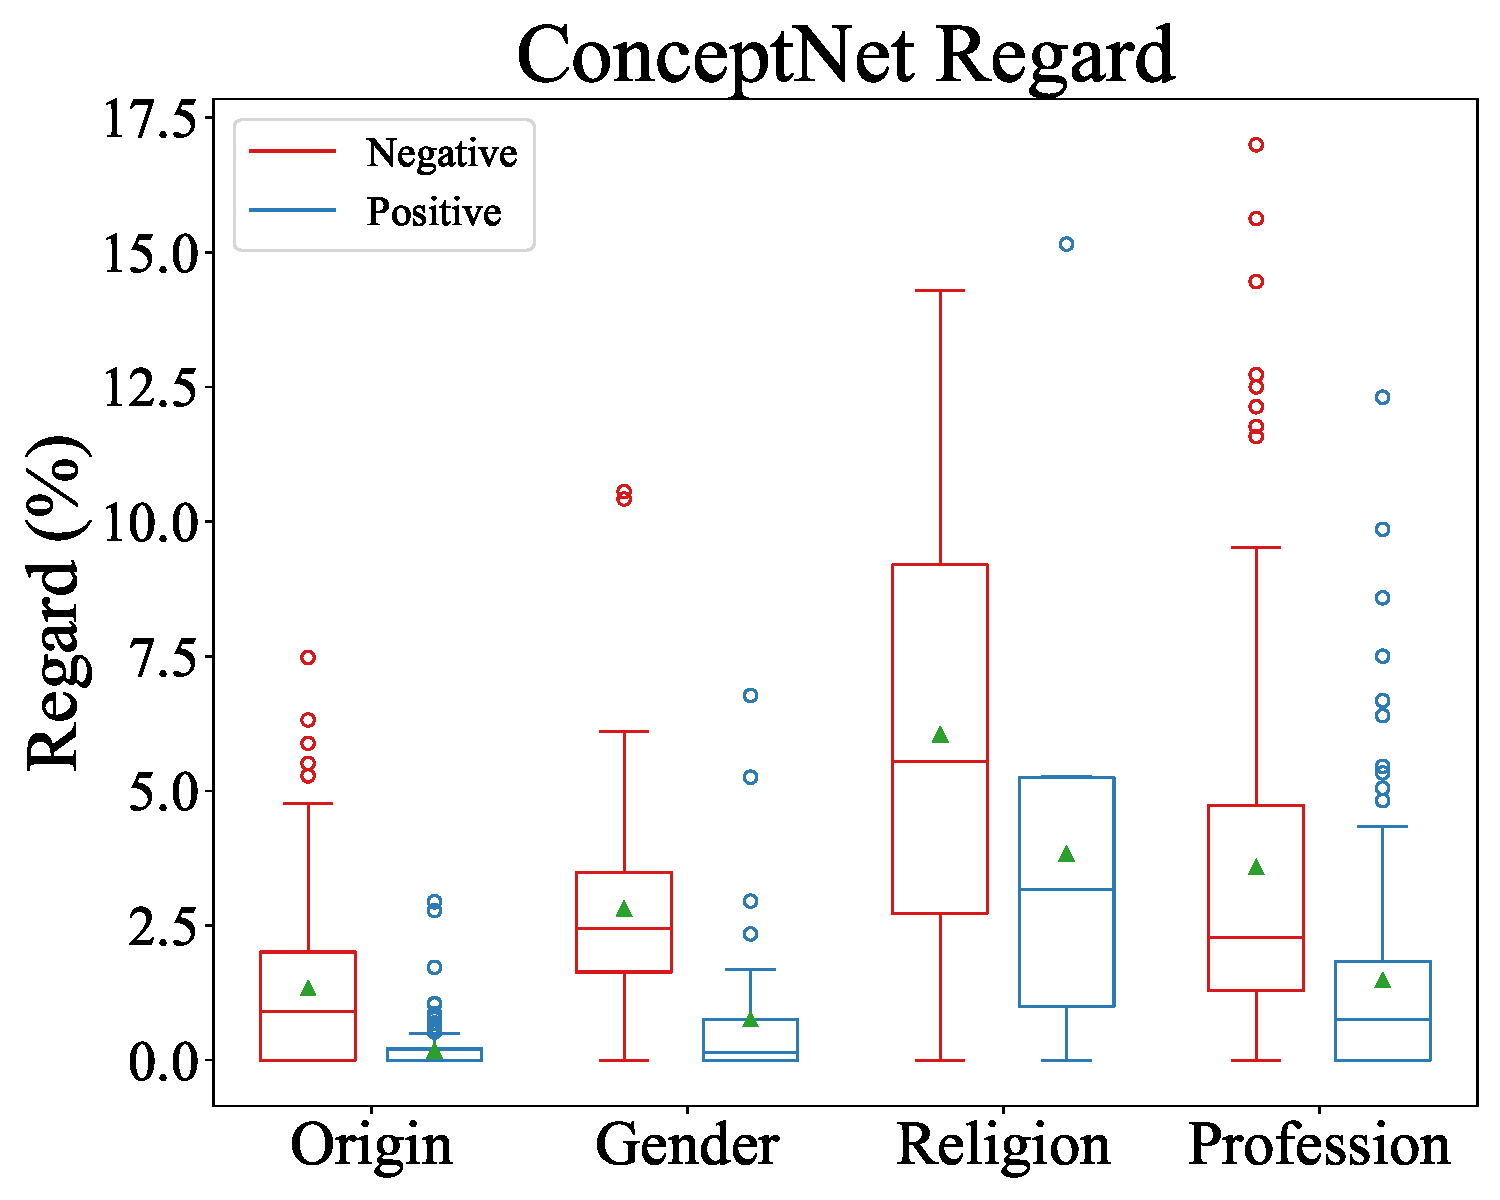
\includegraphics[width=\textwidth,trim=0cm 0cm 0cm 0cm,clip=true]{./images/conceptnet_regard_new_layout.pdf}
\end{subfigure}
\begin{subfigure}[b]{0.24\textwidth}
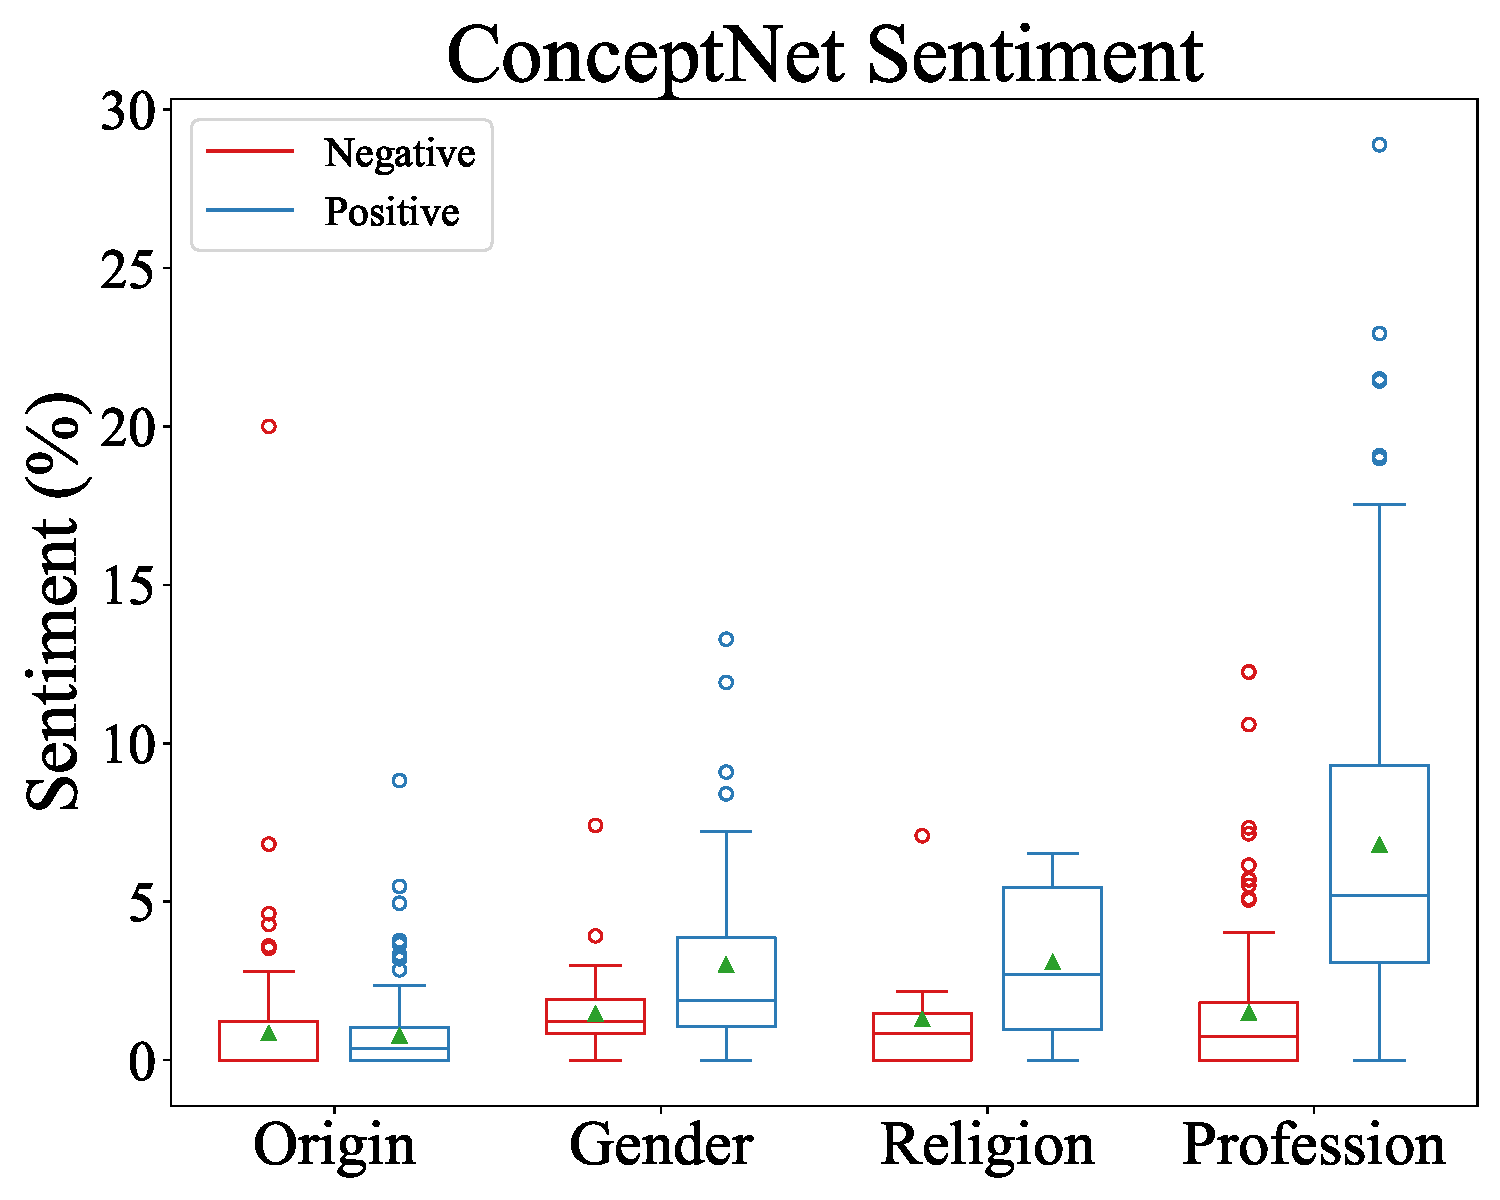
\includegraphics[width=\textwidth,trim=0cm 0cm 0cm 0cm,clip=true]{./images/conceptnet_sentiment_new_layout.pdf}
\end{subfigure}
\begin{subfigure}[b]{0.24\textwidth}
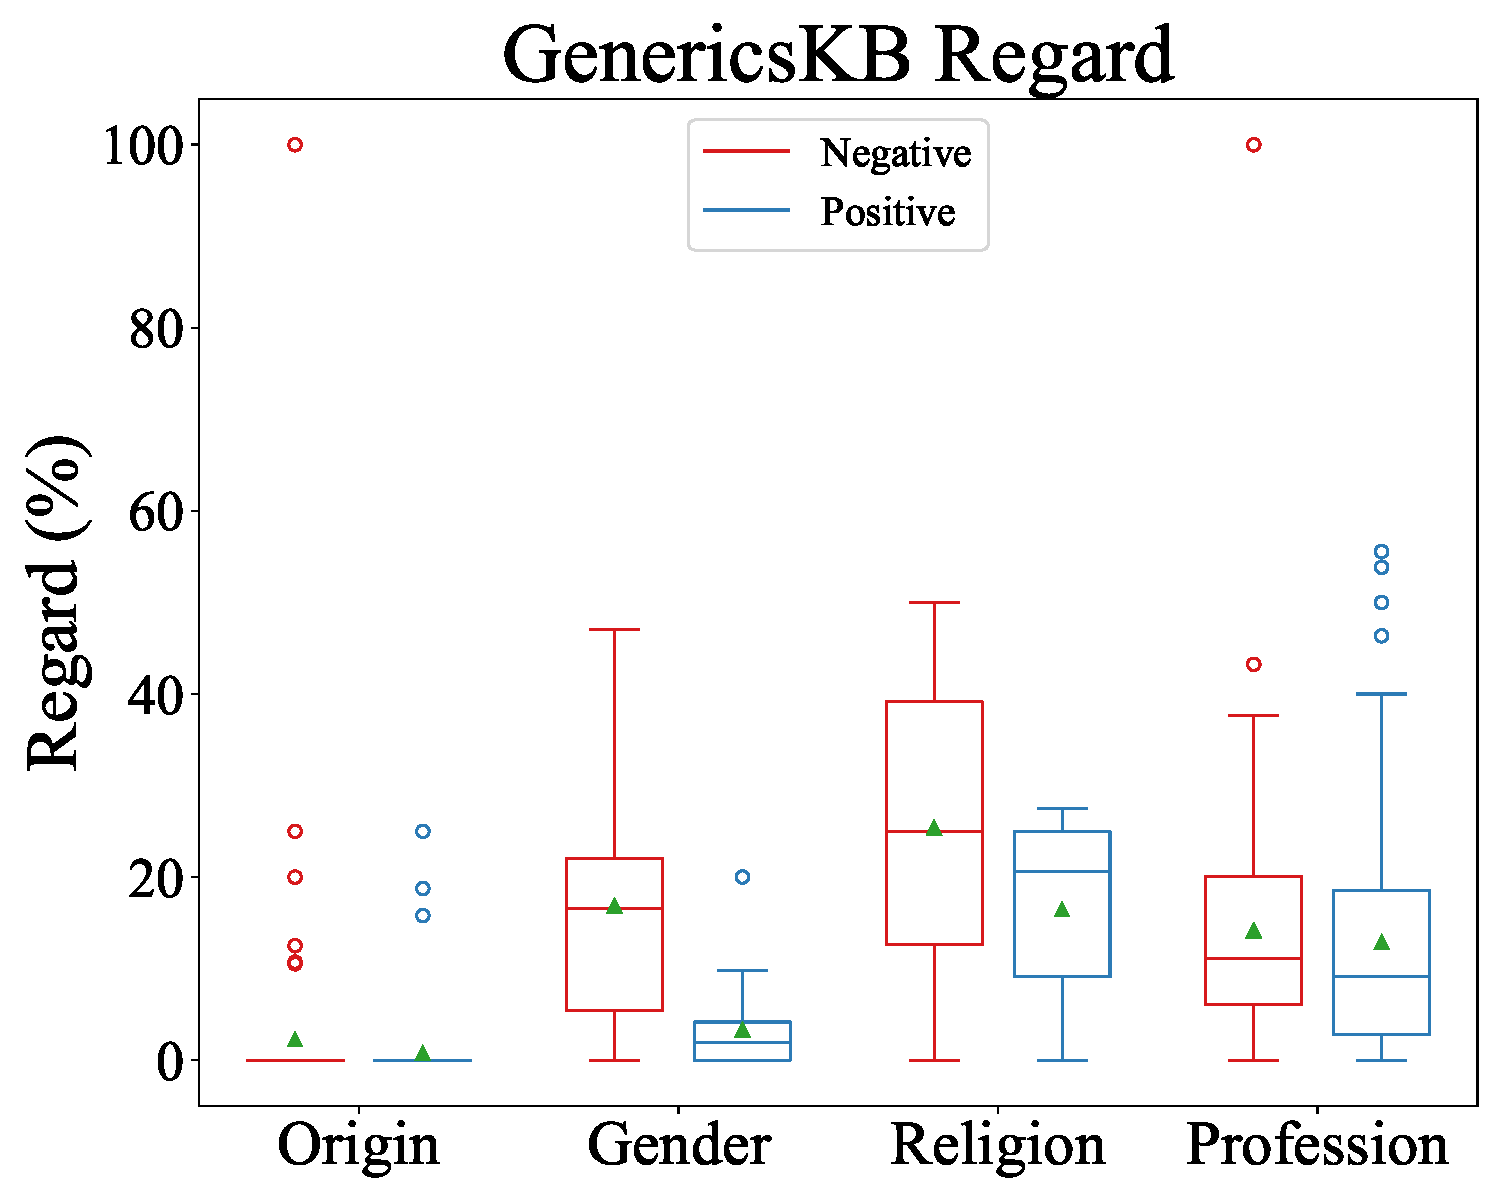
\includegraphics[width=\textwidth]{./images/GenericsKB_regard.pdf}
\end{subfigure}
\begin{subfigure}[b]{0.24\textwidth}
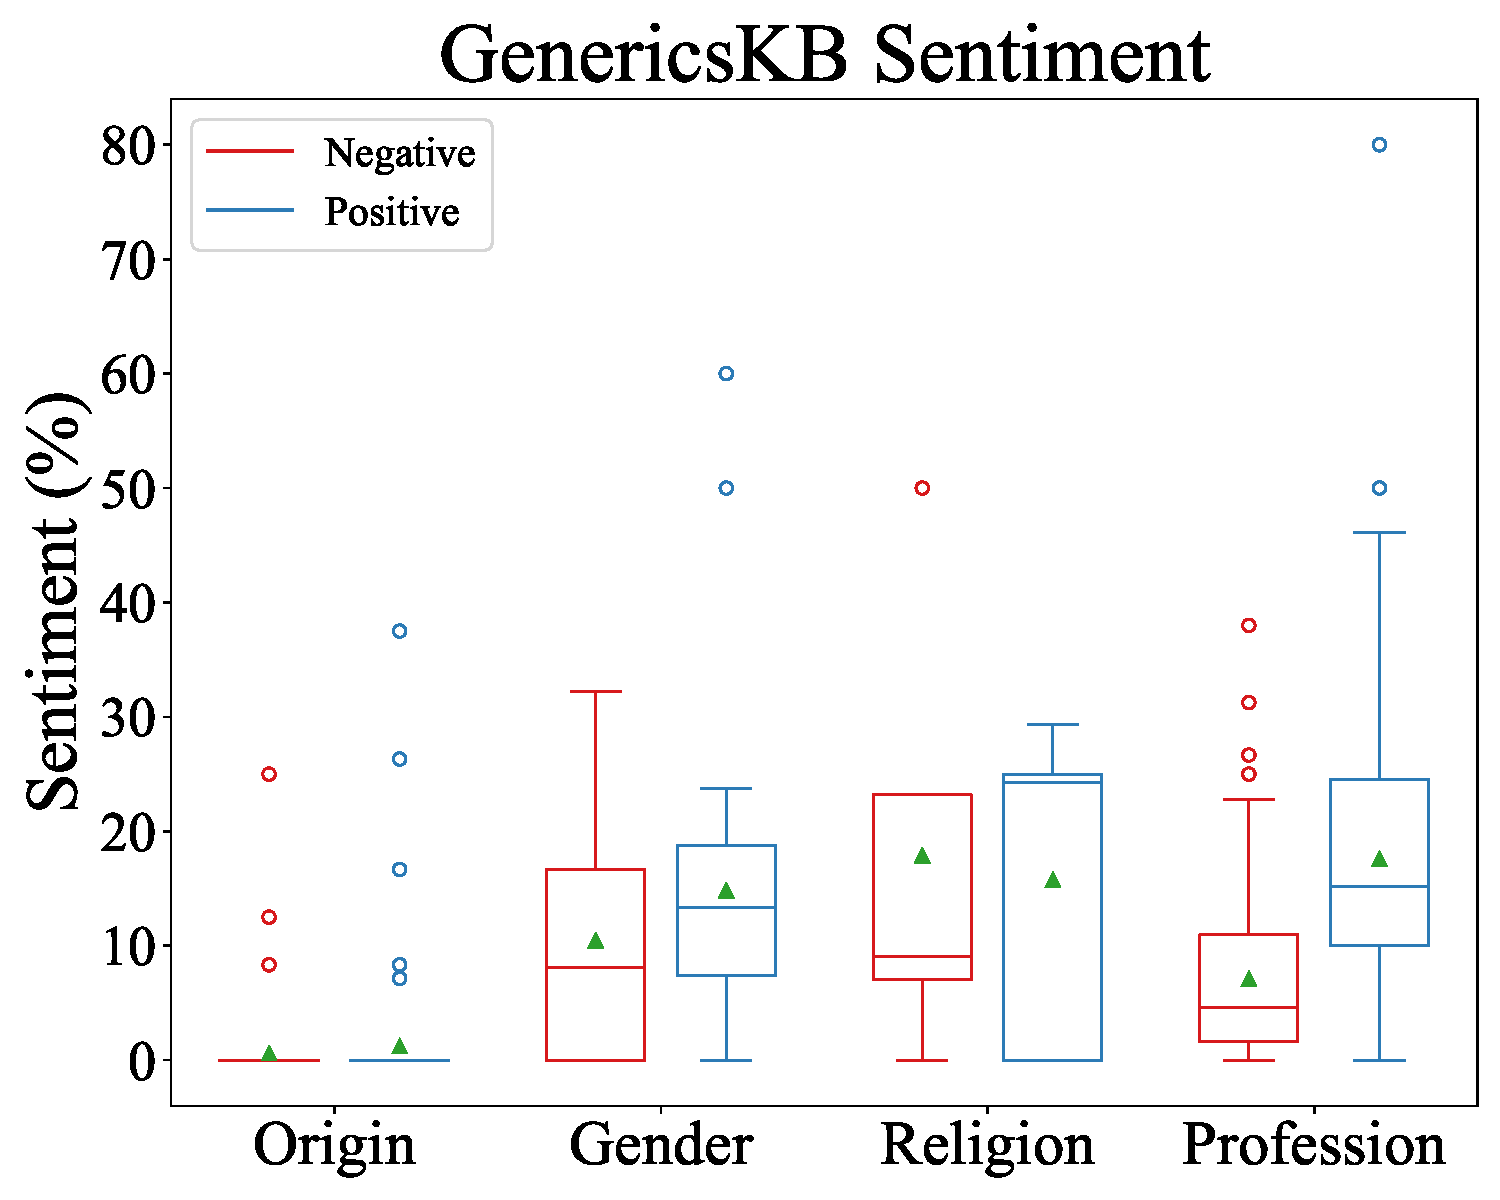
\includegraphics[width=\textwidth]{./images/GenericsKB_sentiment.pdf}
\end{subfigure}

\caption{Negative and positive regard and sentiment results from ConceptNet and GenericsKB. We find outlier target groups with high regard and sentiment percentages that show the severity of \textbf{overgeneralization} issues. We also find large \textbf{variation/disparity} in the number of negative or positive triples for groups in the same category indicated by the span of boxes.
}
\label{fig:Conceptnet_Bias_results}
\end{figure*}
\begin{figure*}[h]
% \centering
\begin{subfigure}[b]{0.33\textwidth}
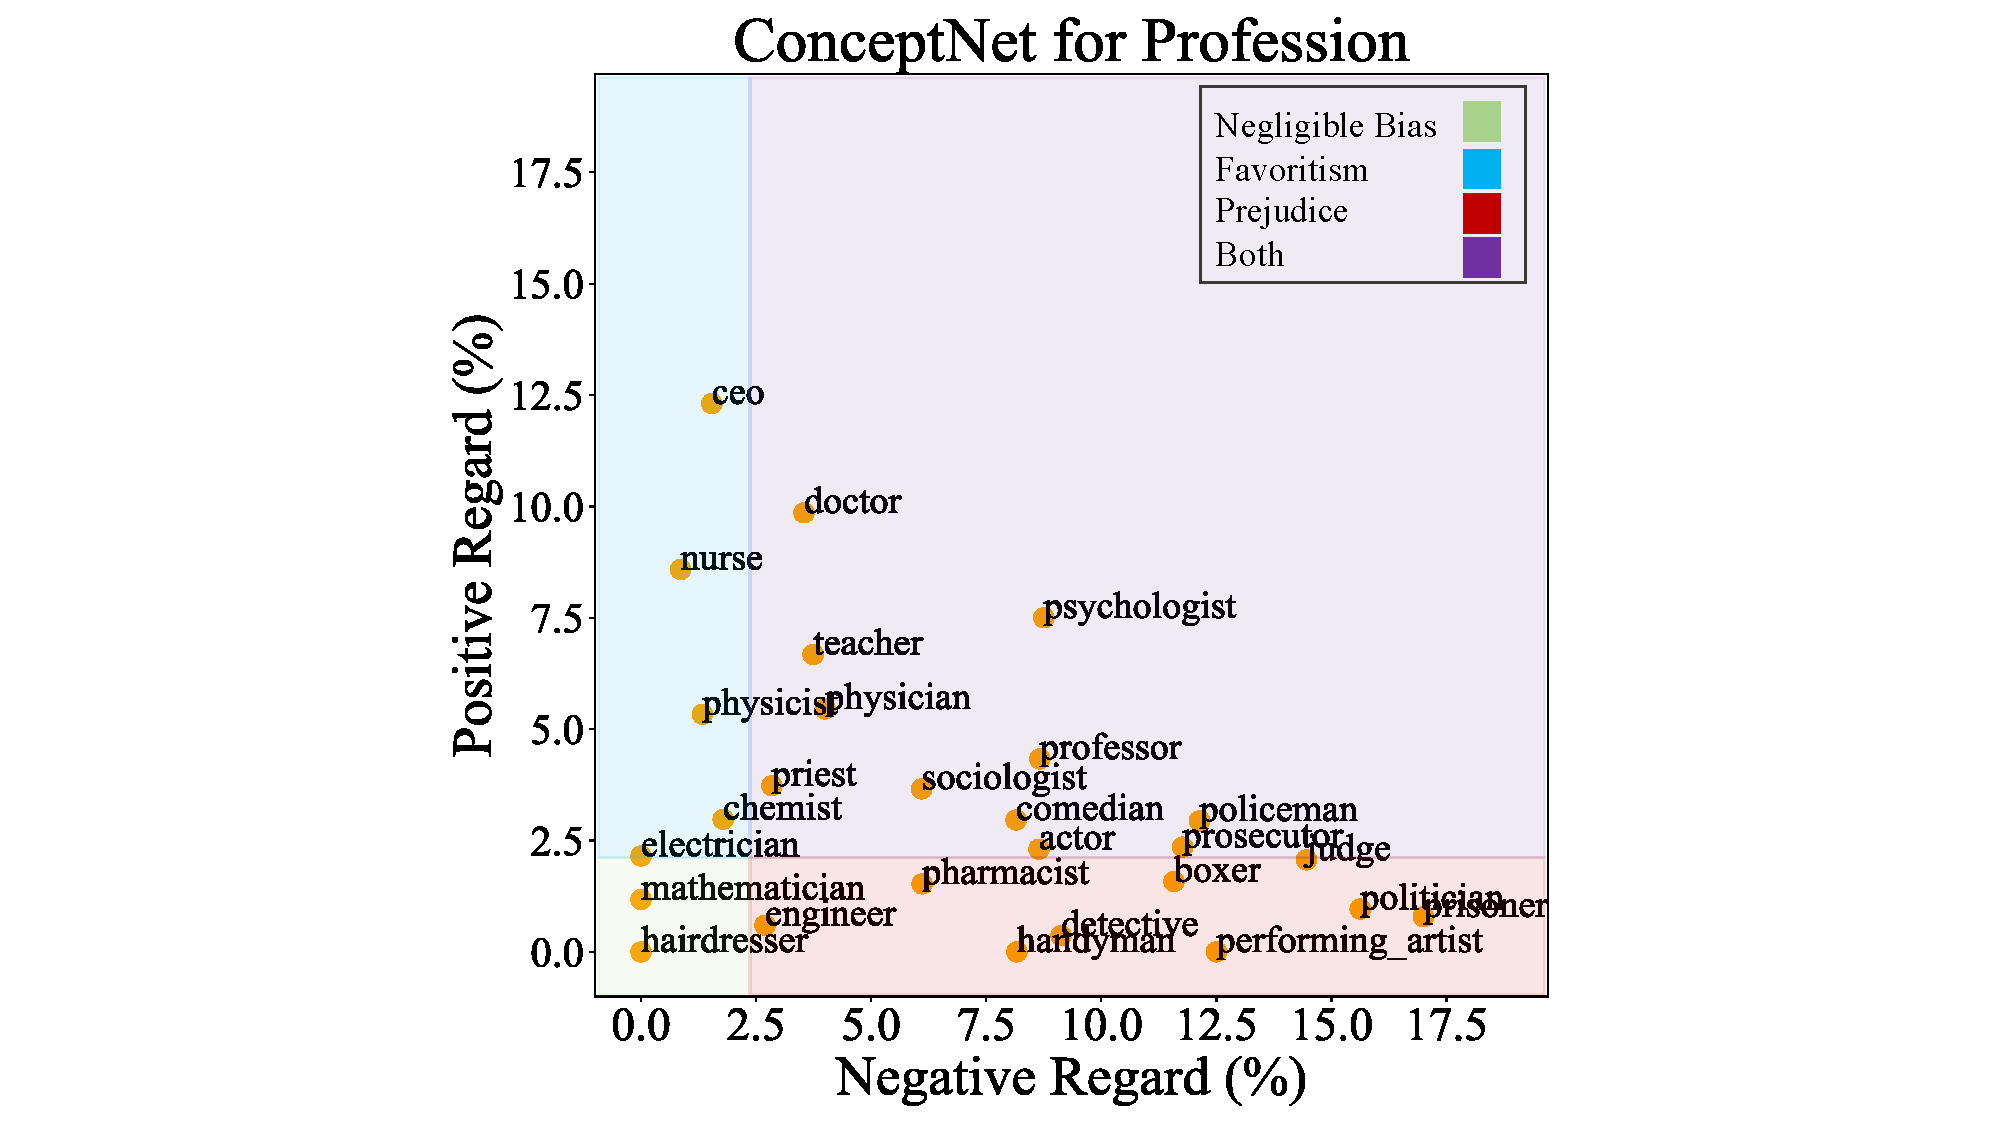
\includegraphics[width=\textwidth,trim=7.3cm 0cm 7.3cm 0cm,clip=true]{./images/large_new_ex_scatter.pdf}
\end{subfigure}
\begin{subfigure}[b]{0.33\textwidth}
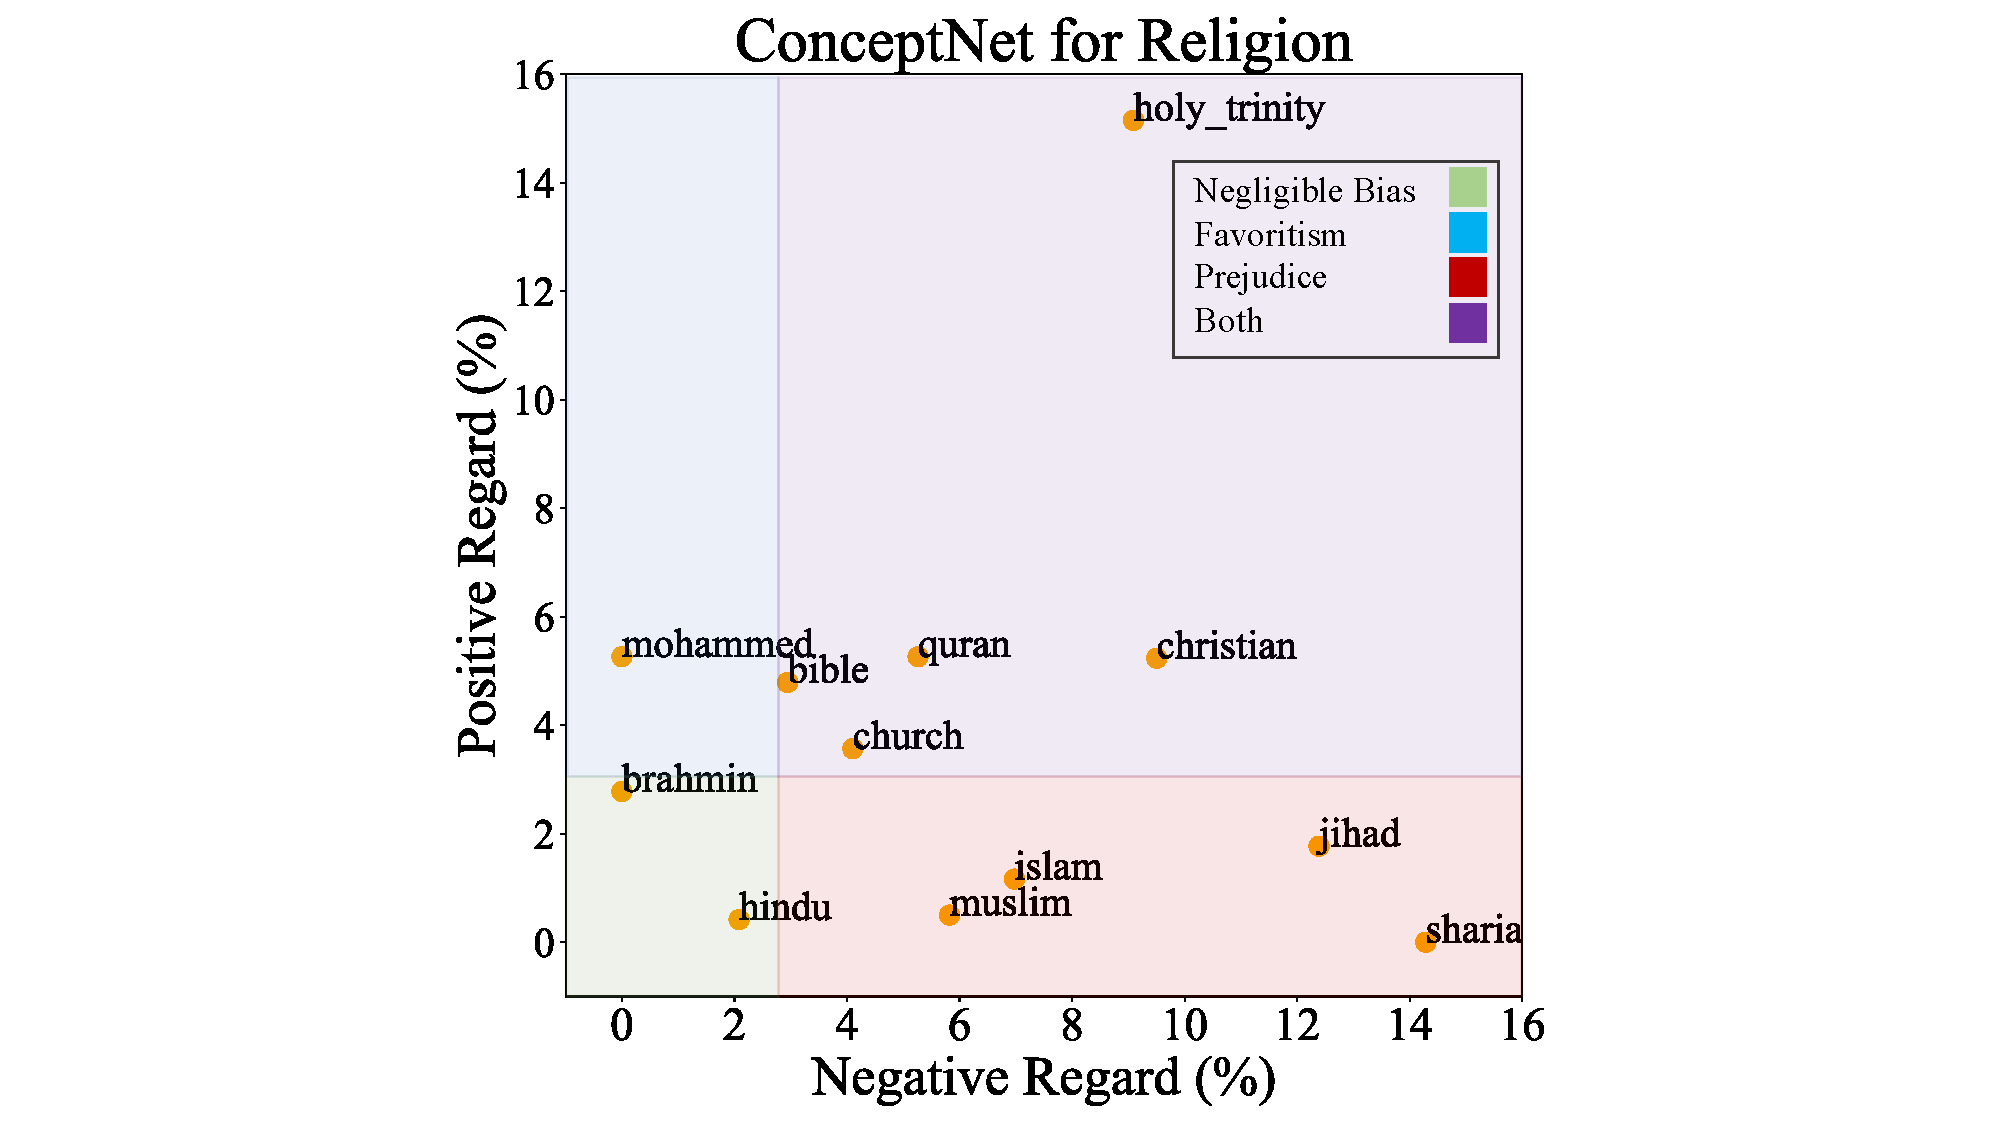
\includegraphics[width=\textwidth,trim=7.3cm 0cm 7.3cm 0cm,clip=true]{./images/large_new_relig_scatter.pdf}
\end{subfigure}
\begin{subfigure}[b]{0.33\textwidth}
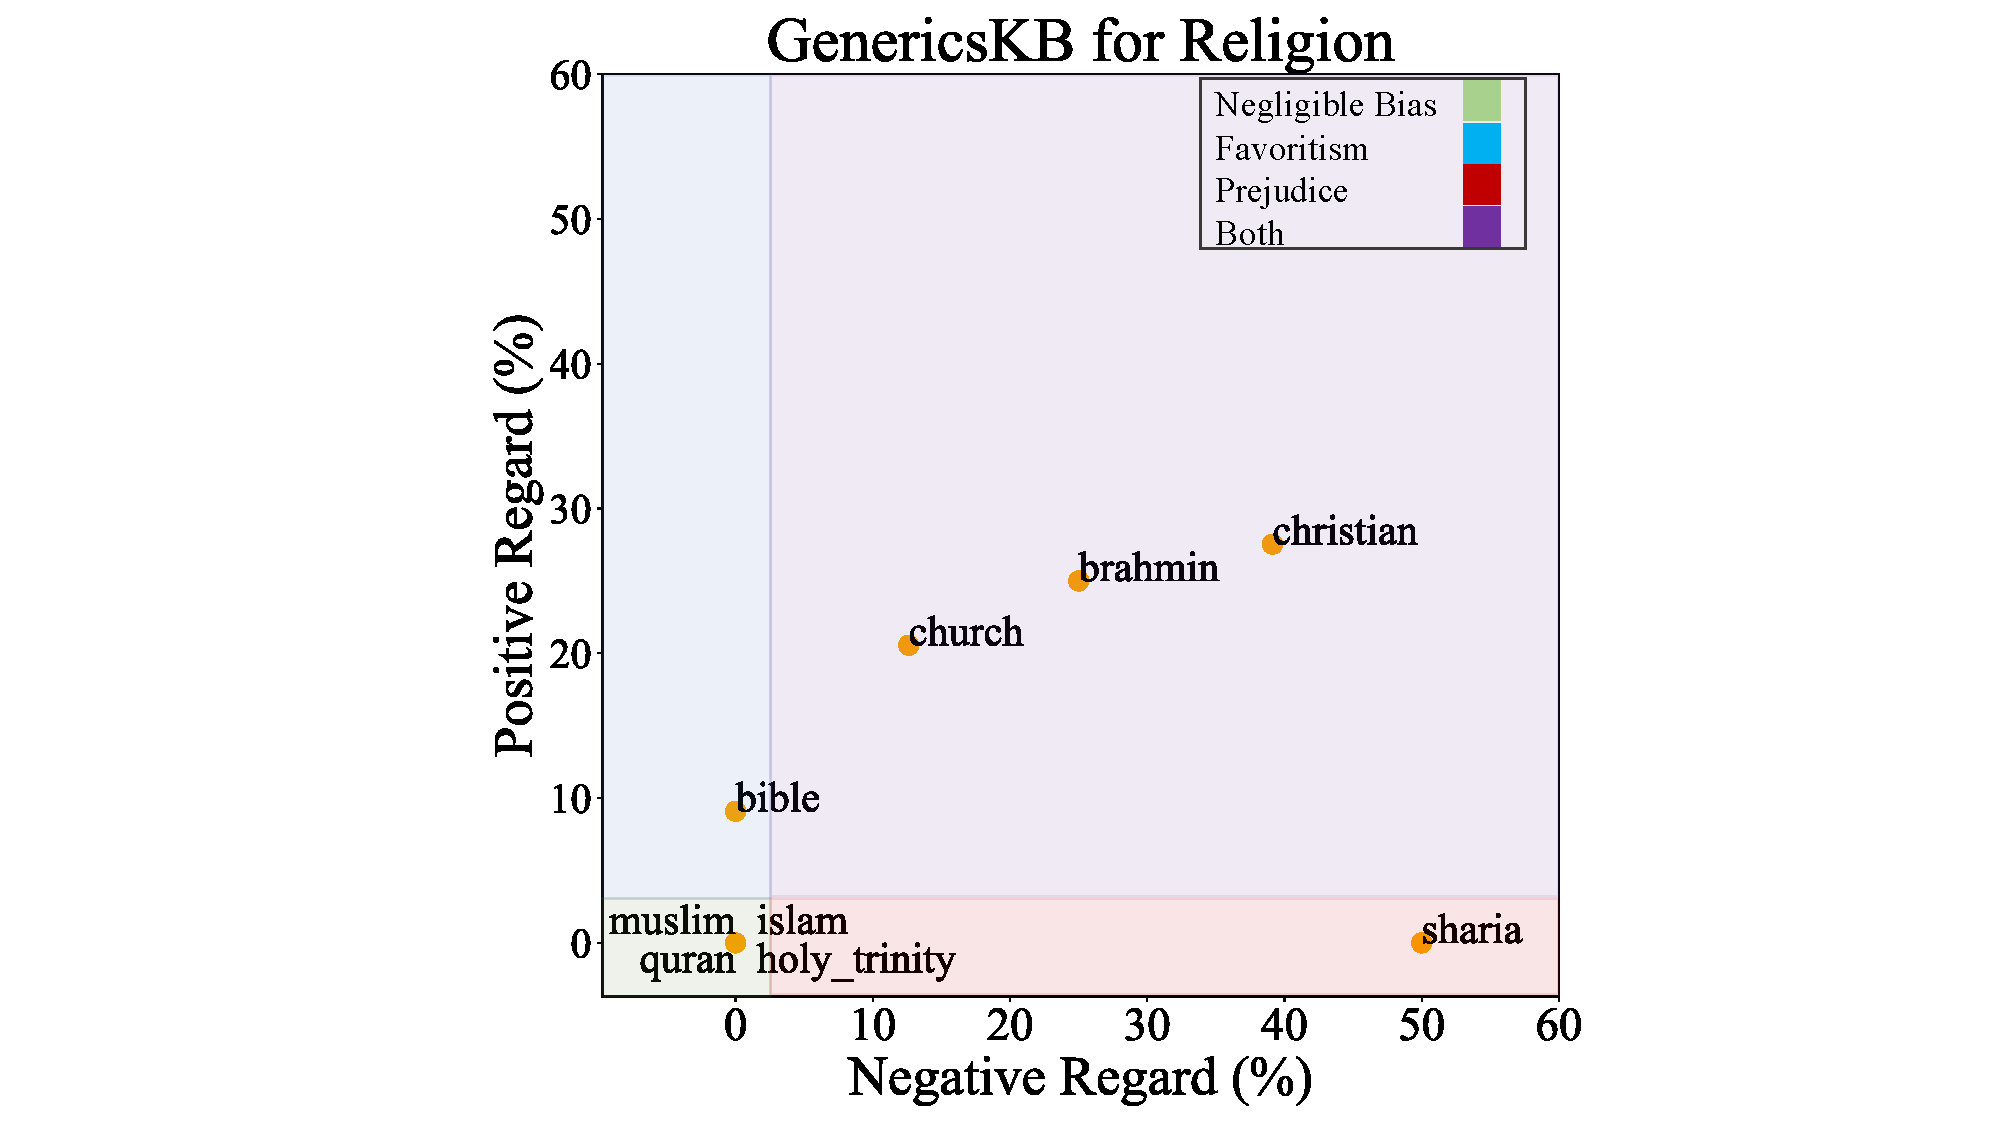
\includegraphics[width=\textwidth,trim=8.3cm 0cm 6.3cm 0cm,clip=true]{./images/GKB_religion_scatter_uncropped.pdf}
\end{subfigure}
\caption{Examples of targets from the ``\emph{Profession}'' and ``\emph{Religion}'' categories from~\citet{nadeem2020stereoset} labeled by the regard measure. Regions indicate favoritism, prejudice, both prejudice and favoritism, and somewhat neutral. Higher negative regard percentages indicate prejudice-leaning and higher positive regard percentages indicate favoritism-leaning. We also compare ConceptNet~\cite{speer2017conceptnet} and GenericsKB~\cite{bhakthavatsalam2020genericskb} on the ``\emph{Religion}'' category and find similar polarized perceptions of certain groups, despite a much larger percentage range for GenericsKB.}
\label{fig:scatter_prof_sent}

\end{figure*}



\begin{figure*}[h]
\centering
% 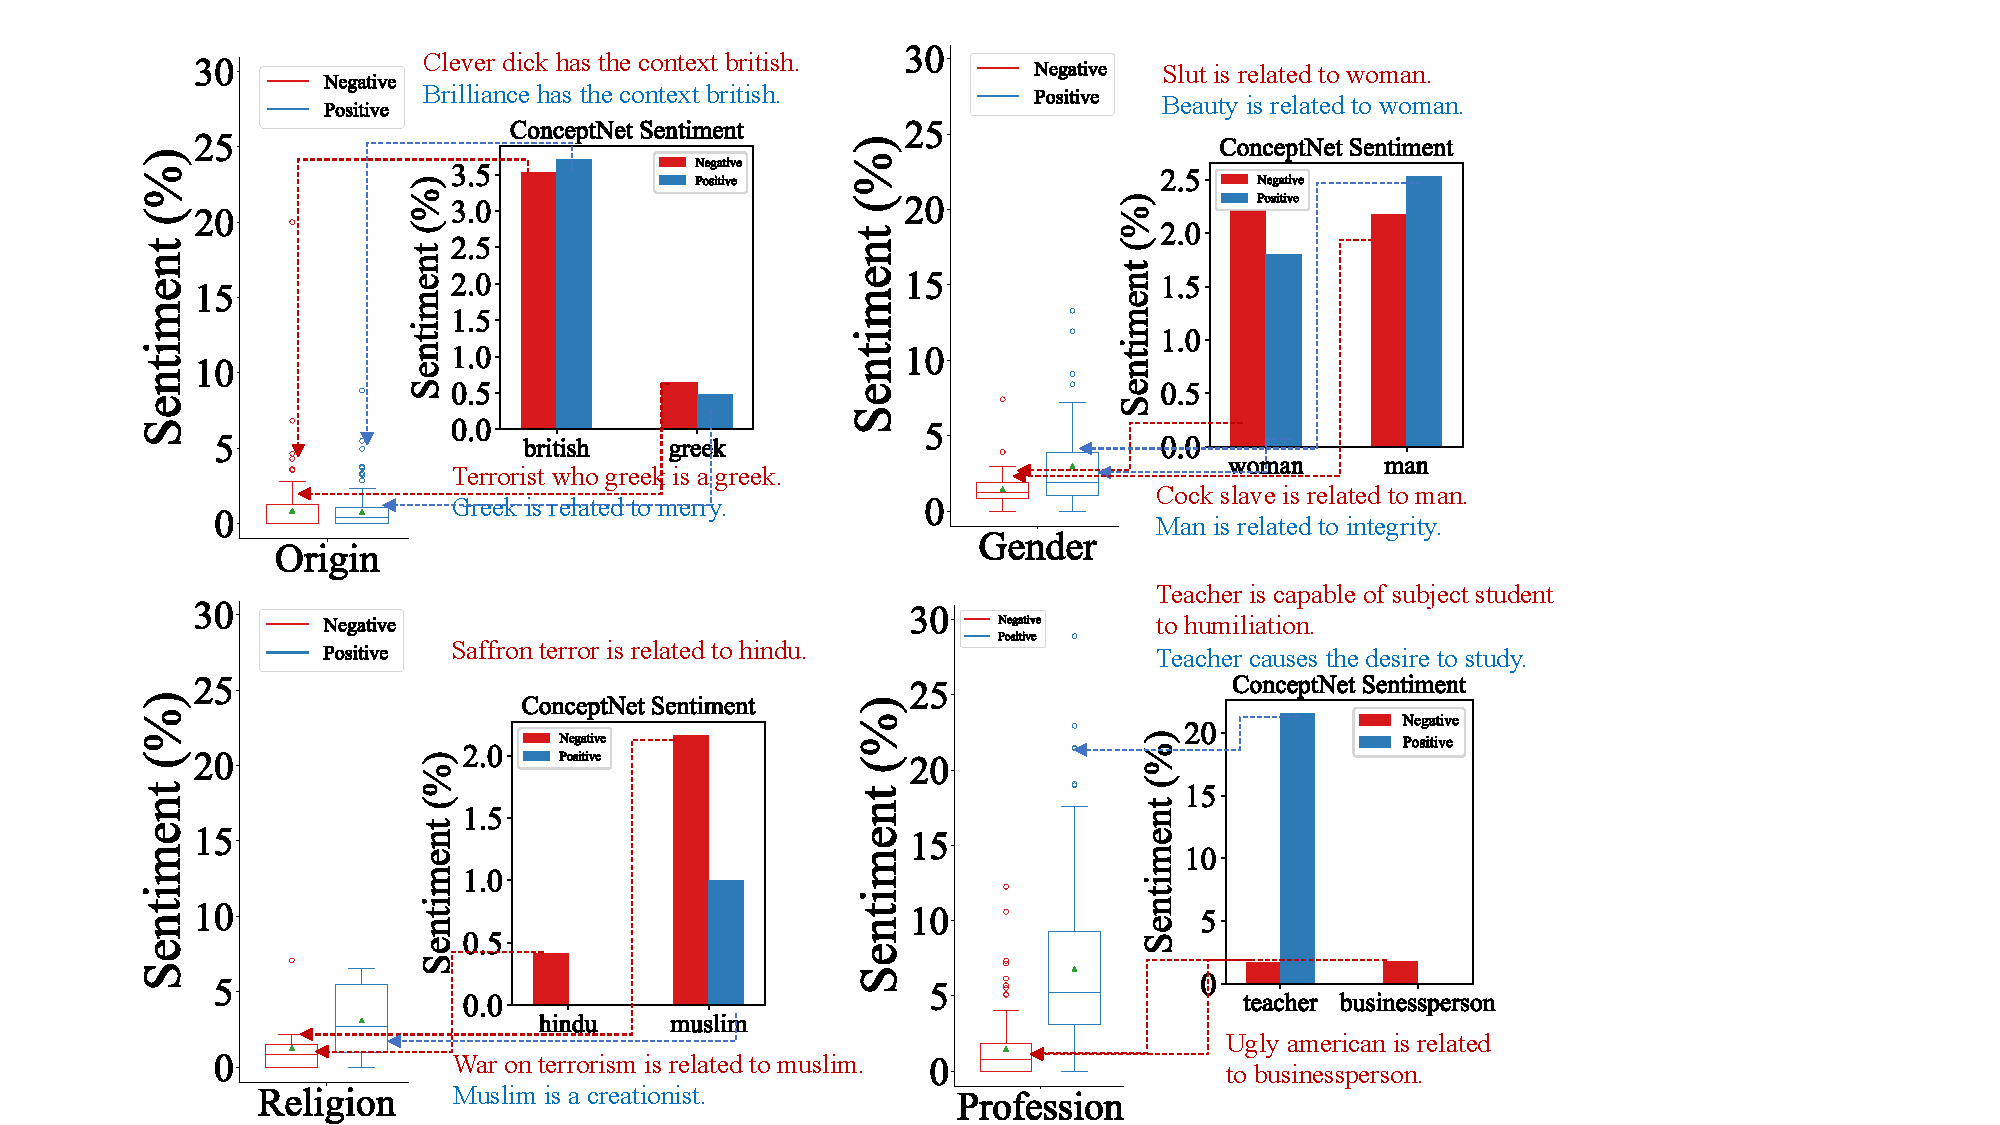
\includegraphics[width=0.8\textwidth,trim=2cm 0cm 7.5cm 0cm,clip=true]{./images/new_bar_plots2.pdf}
\begin{subfigure}[b]{0.49\textwidth}
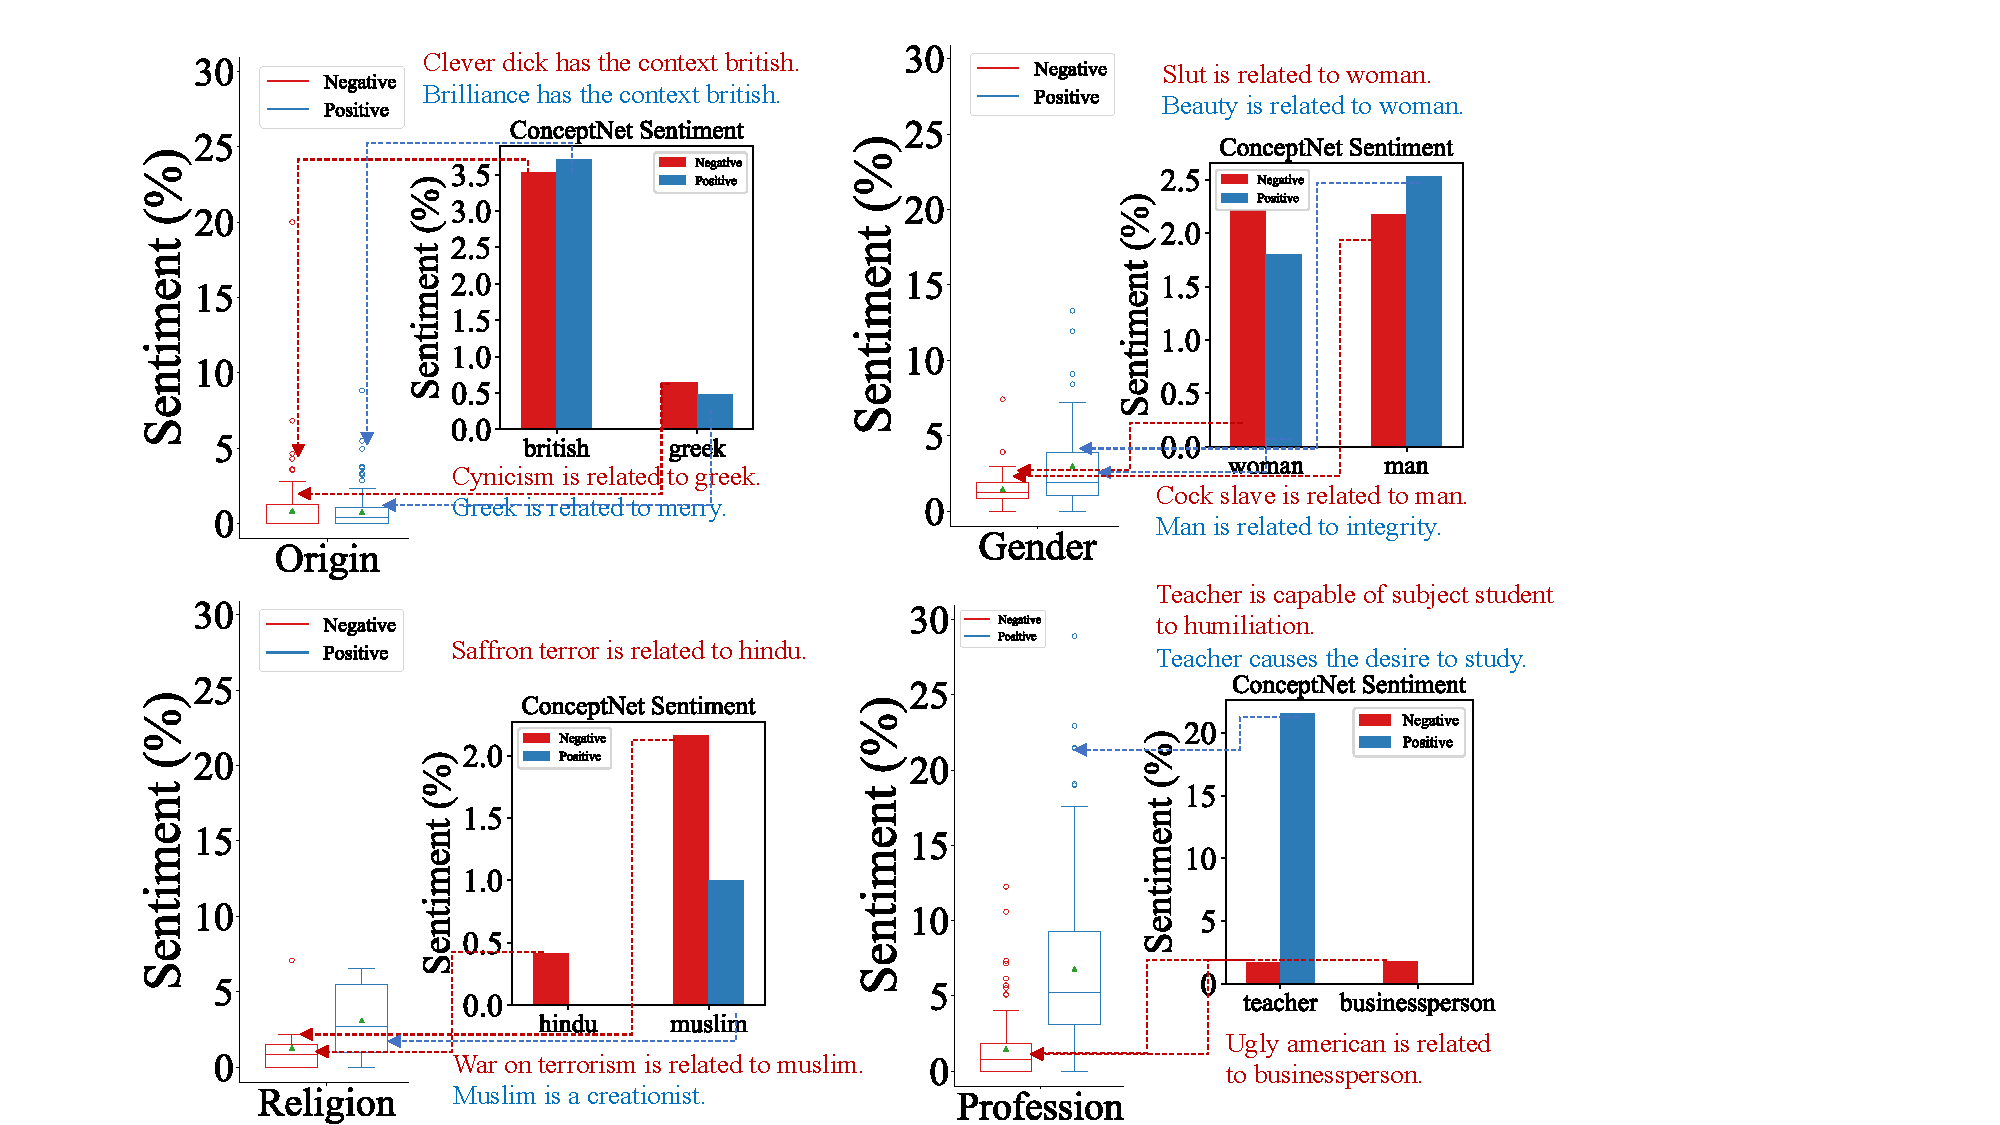
\includegraphics[width=\textwidth,trim=2cm 9.2cm 9cm 0cm,clip=true]{./images/new_small_new_bar_plots.pdf}
\end{subfigure}
\begin{subfigure}[b]{0.49\textwidth}
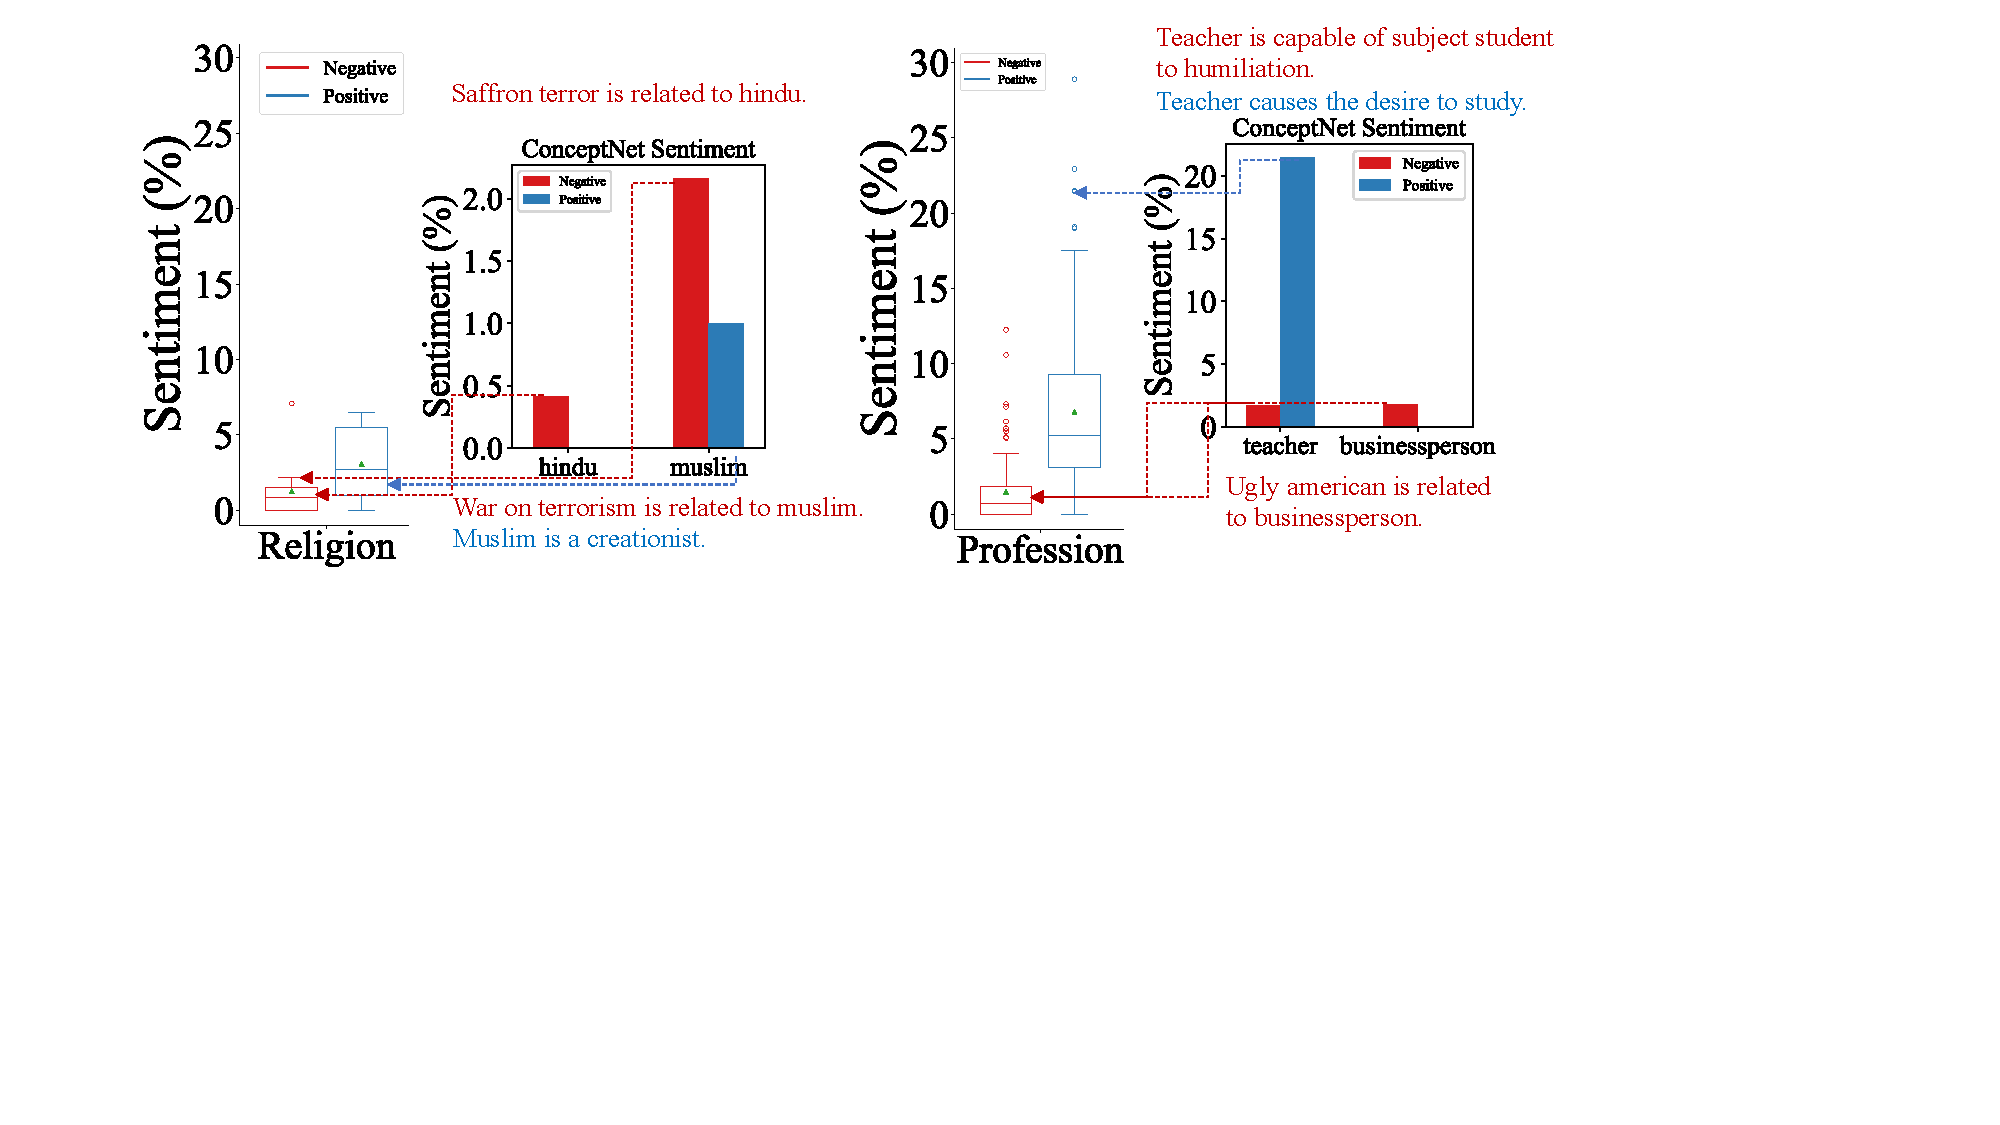
\includegraphics[width=\textwidth,trim=2cm 9cm 7.5cm 0cm,clip=true]{./images/small_new_bar_plots2.pdf}
\end{subfigure}
\caption{Four different representations from four categories each demonstrating a certain aspect of bias. In ``\emph{Origin}'' category, we can observe extreme overgeneralization toward ``\emph{british},'' in ``\emph{Gender}'' category both target groups are overgeneralized, in ``\emph{Religion}'' extreme prejudice toward ``\emph{muslim},'' and in ``\emph{Profession}'' extreme favoritism toward ``\emph{teacher}'' target group. Each case is accompanied with an example of negative and positive associations detected by sentiment.
}
\label{fig:sample_Bias_results}
\end{figure*}


\begin{figure}[h]
\centering
\begin{subfigure}[b]{0.24\textwidth}
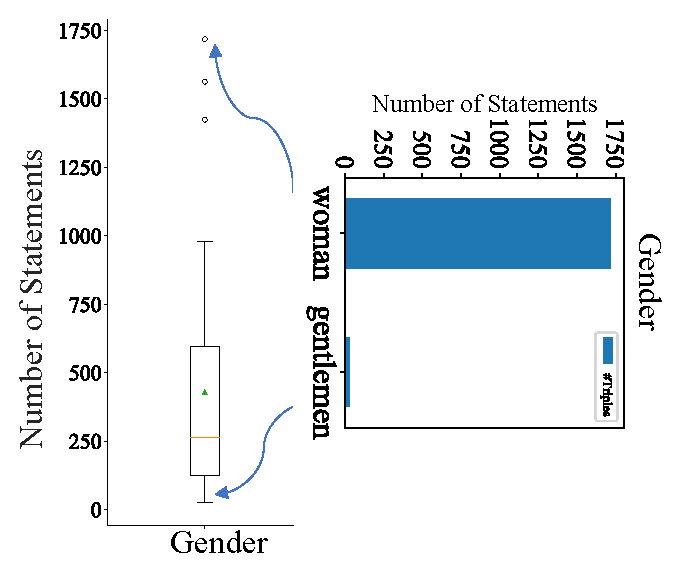
\includegraphics[width=\textwidth,trim=0.2cm 0.2cm 0.2cm 0.2cm,clip=true]{./images/freq_ex_gender.pdf}
\caption{ConceptNet Gender}
\end{subfigure}
\begin{subfigure}[b]{0.22\textwidth}
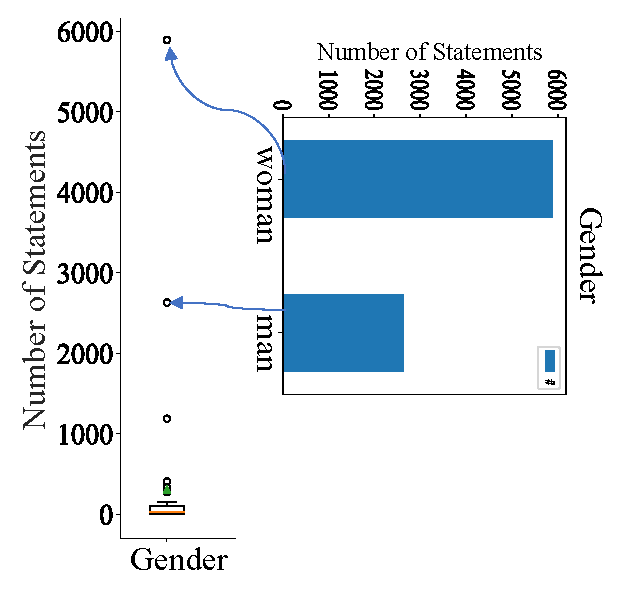
\includegraphics[width=\textwidth,height=0.13\textheight,trim=0.2cm 0.2cm 0.2cm 0.2cm,clip=true]{./images/freq_GKB_gender_cropped.pdf}
\caption{GenericsKB Gender}
\end{subfigure}
\begin{subfigure}[b]{0.23\textwidth}
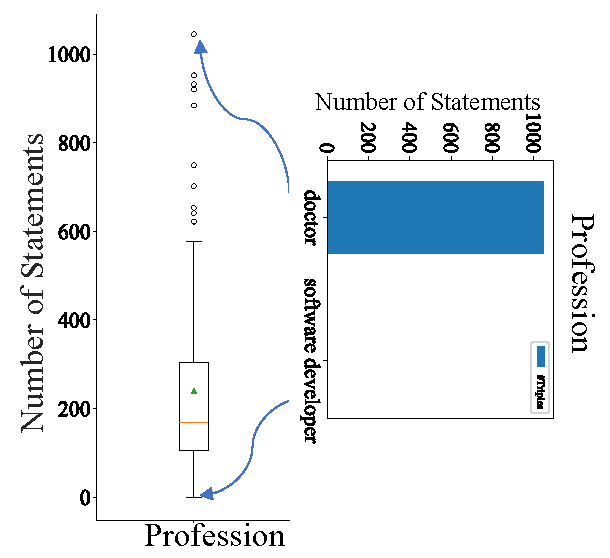
\includegraphics[width=\textwidth,trim=0.2cm 0.2cm 0.2cm 0.2cm,clip=true]{./images/freq_ex_prof.pdf}
\caption{ConceptNet Profession}
\end{subfigure}
\begin{subfigure}[b]{0.23\textwidth}
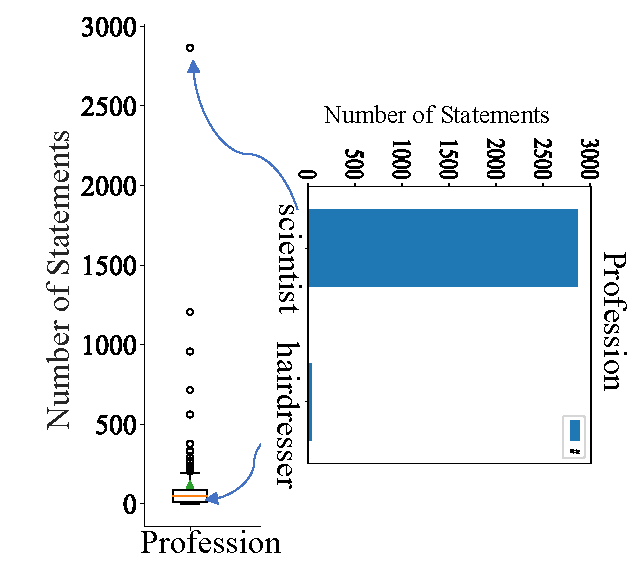
\includegraphics[width=\textwidth,trim=0.2cm 0.4cm 0.2cm 0.2cm,clip=true]{./images/freq_GKB_prof_cropped.pdf}
\caption{GenericsKB Profession}
\end{subfigure}
% \begin{subfigure}[b]{0.15\textwidth}
% \includegraphics[width=\textwidth,trim=0cm 0cm 0cm 0cm,clip=true]{./images/conceptnet_bar_plot_sent_prof.pdf}
% \end{subfigure}
% \begin{subfigure}[b]{0.15\textwidth}
% \includegraphics[width=\textwidth,trim=0cm 0cm 0cm 0cm,clip=true]{./images/conceptnet_bar_plot_regard_prof.pdf}
% \end{subfigure}
\caption{Box plots demonstrating the \textbf{representation disparity} in terms of number of triples/sentences for ``\emph{Gender}'' and ``\emph{Profession}'' categories from ConceptNet and GenericsKB. We find similarly severe disparities in two KBs with the number of sentences ranging much more for GenericsKB compared to ConceptNet.}
\label{fig:sample_freq_results}
\end{figure}

Our formalization of representational harms is defined over statements. GenericsKB uses naturally occurring sentences, so our measures (in Sec.~\ref{sec:formalization}) directly apply. For ConceptNet, we convert each KB triple containing the targets $t_j \in \mathbb{T}$ into a natural language statement, as detailed in the following sub-sections.


\subsection{Data Preparation}

\noindent
\textbf{Selection of Target Groups}
% \para{Data}
Let $G$ be the graph of the CSKB that consists of commonsense assertions in the form of triples $(s,r,o)$ representing ``\emph{subject-relation-object}''. Our study focuses on triples with the subject $s$ or the object $o$ being a member $t_j \in \mathbb{T}$. 
% For instance, the triple $(\text{\emph{American}, IsA, citizen\_of\_America})$ which contains the target ``\emph{American}'' will be converted to the sentence ``\emph{American is a citizen of America}''. 
We first collect a list of targets $t_j$ from the StereoSet dataset~\cite{nadeem2020stereoset}. The collected targets are organized within 4 different categories: \textit{origin}, \textit{gender}, \textit{religion}, and \textit{profession}. We renamed the ``\emph{race}'' category from ~\cite{nadeem2020stereoset} to ``\emph{origin}'' to be more precise as words such as \textit{British} may not necessarily represent a race but more of the origin or nationality of a person. Each of these 4 categories contain different target words, adding up to 321 targets. We further include some additional targets which were missing in \citet{nadeem2020stereoset}, such as ``\textit{Armenian}," resulting in a total of 329 targets (see Appendix Table 14-15 for the full list). 

\para{Collection of CSKB Triples}
We collect all the triples from ConceptNet 5.7\footnote{\url{https://github.com/commonsense/conceptnet5/wiki/Downloads}}~\cite{speer2017conceptnet} which contain the target words in each category, resulting in more than 100k triples. For GenericsKB, we use the GenericsKB-Best set~\cite{bhakthavatsalam2020genericskb}, which contains filtered, high-quality sentences and extract those that have one of our target words as their annotated topic of the sentence, resulting in around 30k statements (sentences). 

\para{Converting Triples to Statement Sentences} 
We convert every triple to a sentence by mapping the relation $r$ in the triple to its natural language form $\Tilde{r}$, and concatenate $s$, $\Tilde{r}$, and $o$ to be a statement $s_i$ in $\mathbb{S}$. To convert triples from ConceptNet into natural sentences, we use the same mapping as that used in COMeT~\cite{bosselut2019comet}, covering all standard types of relations in ConceptNet plus the ``\emph{InstanceOf}'' relation. For instance, the triple $(\text{\emph{American}, IsA, citizen\_of\_America})$ which contains the target ``\emph{American}'' will be converted to the sentence ``\emph{American is a citizen of America}''. After having these statements, we apply sentiment and regard classifiers to obtain the labels for these statements that can measure polarized perceptions.

\para{Quantifying Harms}
During the classification process using sentiment and regard classifiers, we mask all the demographic information from the sentences to avoid biases in sentiment and regard classifiers that may affect our analysis. We obtain sentiment and regard labels for the masked sentences using the VADER sentiment analysis tool \cite{gilbert2014vader} which is a rule-based sentiment analyzer. For regard, we use the fine-tuned BERT model from \cite{sheng2019woman}. After obtaining the labels, we use Eq.~(1) and (2) to measure overgeneralization and Eq.~(4) for disparity in overgeneralization.



\subsection{Analysis of Representational Harms}
\noindent
\textbf{Results on Overgeneralization}
%\pei{maybe we should organize the analysis better by separating into a few headlines so that reviewers can get the key takeaways easily (R1 points out similar issues)}
We quantify overgeneralization using Eq.~(1) and (2) in Section~\ref{sec:formalization}. The overall average percentage of overgeneralized triples in ConceptNet is 4.5\% (4.6k triples) for sentiment and 3.4\% (3.6k triple) for regard.
% in other words, around 4,600 triples are biased according to sentiment, and 3,600 according to regard. 
For GenericsKB, the percentages are 36.5\% for sentiment (11k triples) and 38.6\% for regard (11k triples). 
% meaning around 10,756 triples are biased according to sentiment, 
% and 11,399 according to regard. 
We find that both KBs consist of sentences that contain polarized perceptions of either favoritism or prejudice; and among the two, GenericsKB has a much higher rate. 

In a closer look, Figure~\ref{fig:Conceptnet_Bias_results} presents the box plots of negative and positive regard/sentiment percentages for targets in 4 categories for both CSKBs. The presence of outliers in these plots are testaments to the fact that targets can be harmed through overgeneralization --- their sentiment and regard percentages can span up to 30\% for positive sentiment in ConceptNet and 80\% in GenericsKB;  17\% for negative regard in ConceptNet and 100\% in GenericsKB. We again find some similar trends of representational harms across the two KBs qualitatively, such as the box shapes for ``\emph{Gender}'' and ``\emph{Religion}'' categories, indicating common biases in knowledge resources. Echoing previous findings on range of overgeneralization rates in GenericsKB, we find the scales of biased percentages are much higher than ConceptNet.


\para{Regions of Overgeneralization}
By plotting the negative and positive regard percentages for each target along the x and y coordinates, Figure~\ref{fig:scatter_prof_sent} demonstrates the issue of overgeneralization in different categories. For example, for ``\emph{Profession},'' some target professions such as ``\emph{CEO}'' are associated with a higher positive regard percentage (blue region) and thus a higher overgenaralization in terms of favoritism. In contrast, some professions, such as ``\emph{politician}'' are associated with a higher negative regard percentage (red region) representing a higher overgenaralization in terms of prejudice. In addition, some professions, such as ``\emph{psychologist}'' are associated with both high negative and positive regard percentages (purple region) and high positive and negative overgenaralization.


\para{ConceptNet vs GenericsKB}
We compare ConceptNet and GenericsKB on the ``\emph{Religion}'' category and see certain targets contain similar biases, such as ``\emph{christian}'' contains both biases and ``\emph{sharia}'' is prejudiced against in both KBs. Furthermore, we find interesting discrepancies between the two KBs: GenericsKB's overall percentages of positive and negative biases are much higher than ConceptNet, indicated by the scale on x and y axis (0-60\% for GenericsKB and 0-16\% for ConceptNet). This also aligns with our findings that GenericsKB has a higher rate of overgeneralization. 
%This is the case when some professions like ``\emph{hairdresser} are located near the center belonging to the acceptable bias region.


% This is while some targets have 0\% negative and positive sentiment/regard percentages. 

\para{Severity of Overgeneralization}
Figure~\ref{fig:sample_Bias_results} further demonstrates how severe the problem of overgeneralization can be, along with some concrete examples. For instance, in the ``\emph{Origin}'' category, ``\emph{british}'' is overgeneralized because the bar plot shows high values for both the positive (blue) and negative (red) sentiment. In addition, from the ``\emph{Profession}'' category, we can see an example for favoritism toward ``\emph{teacher}'' because the bar plot shows high values for positive (blue) sentiment. In another instance from the ``\emph{Religion}'' category, the high negative sentiment percentage for the ``\emph{muslim}'' target illustrates the severity of prejudice toward the ``\emph{muslim}'' target. 


% We find that both negative and positive overgeneralizations of social perceptions exist in ConceptNet demographic triples according to sentiment and regard scores. The overall average percentage of such unwanted triples is 4.5\% for sentiment and 3.4\% for regard; in other words, around 4,600 triples are biased according to sentiment, and 3,600 according to regard. Specifically, certain groups have very high percentages (30\% for sentiment and 17\% for regard) of overgeneralization indicated by the outlier dots above the boxes. This finding shows that there are non-trivial numbers of triples in ConceptNet overgeneralizing demographics negatively or positively.

%Another interesting trend can be observed by analyzing actual percentages. For instance, for the same negative regard scores, sexual orientation category is associated with higher negative regard percentages compared to religion which can give some intuition to the reader on how categories are different from each other in terms of associations provided to the groups contained in them. To summarize, these plots can provide information about both inter-category and intra-category statistics in terms of disparities amongst different groups within a category as well as across categories.
% We also provide some qualitative results from the existing destructive biases in ConceptNet. The results in Figure \ref{wordcloud_results_conceptnet} show examples of what regard and sentiment detected as negative prejudices against the ``\emph{British}'' target from the ``\emph{Origin}'' category and the ``\emph{female}'' target from the ``\emph{Gender}'' category. As shown in the results, these associations are destructive, biased, and should not be conceived as commonsense knowledge. %From these results, one can also see the differences on what regard and sentiment classifiers each pick up on. While both detect destructive associations correctly, they are somehow different in a sense that sentiment is more focused on the overall polarity of the sentence, while regard picks up on more societal biases. Thus, inclusion of both of these measures can give us better insights and detection mechanisms.

\para{Representation Disparity} 
We first quantify the disparity in terms of the number of triples for each target (word) in the 4 categories, using Eq.~(3). Table~\ref{disparity_table} shows extremely high variance in both CSKBs. Figure~\ref{fig:sample_freq_results} shows the boxplots for the numbers of triples available in ConceptNet and sentences in GenericsKB for different targets within two categories. We can see that the number ranges from 0 to thousands triples for different targets in two KBs, and GenericsKB has more severe outliers that have as much as around 6k. 
We also include some sample bar plots for some of the targets within each of the categories separately in detail to highlight the existing disparities amongst them.

\para{Overgeneralization Disparity}
%\xiang{can we add a small table for just showing the Eq (3)/(4) metrics for the two KBs? Otherwise the metrics weren’t shown until Sec 4.3}

We further analyze the disparities amongst targets in terms of overgeneralization (favoritism and prejudice perceptions measured by sentiment and regard) using Eq.~(4), shown in Table~\ref{disparity_table}. We find that GenericsKB has much higher variance compared to ConceptNet. To better illustrate the disparity, boxplots in Figure \ref{fig:Conceptnet_Bias_results} show the variation of overgeneralization across different groups for 4 categories.
%In addition, we have included the details of negative/positive regard/sentiment percentages for each of the demographic groups inside each of these categories in the form of bar plots in the Appendix section for detailed comparison of the groups for interested readers. They are not included in the main text due to the space limitation. 
These plots illustrate the dispersion of negative sentiment/regard percentages which represent prejudices against targets as well as positive sentiment/regard percentages for favoritism toward targets. We can observe that targets such as``\emph{muslim}'' (shown in Figure~\ref{fig:sample_Bias_results}) may be perceived negatively significantly more than others. The same trend also holds for positive sentiment and regard scores. Figure~\ref{fig:scatter_prof_sent} also shows qualitatively that the targets are not clustered at some point with similar negative and positive regard percentages, but rather spread across different regions.
\begin{table}[t]
\centering
\scalebox{0.63}{
\begin{tabular}{ p{2cm} ccccc}
 \toprule
\textbf{CSKB}&\textbf{Statement \#}&\textbf{Pos Sent}&\textbf{Neg Sent}&\textbf{Pos Reg}&\textbf{Neg Reg}\\
 \midrule
 \parbox[t]{2mm}{\multirow{1}{*}{\shortstack[l]{ConceptNet}}}
&141,538&20.4&4.03&3.74&8.74\\[0.5pt]

 \parbox[t]{2mm}{\multirow{1}{*}{\shortstack[l]{GenericsKB}}} 
&238,277&172&79&131&238\\[0.5pt]
%  \midrule
 \bottomrule
\end{tabular}
}
\caption{Disparity results quantified by \emph{variance} across all targets on two CSKBs as shown in Equations~\ref{eq:3} (statement \#) and~\ref{eq:4}.}
\label{disparity_table}

\end{table}
% \begin{figure*}[h]
% \centering
% \begin{subfigure}[b]{0.4\textwidth}
% 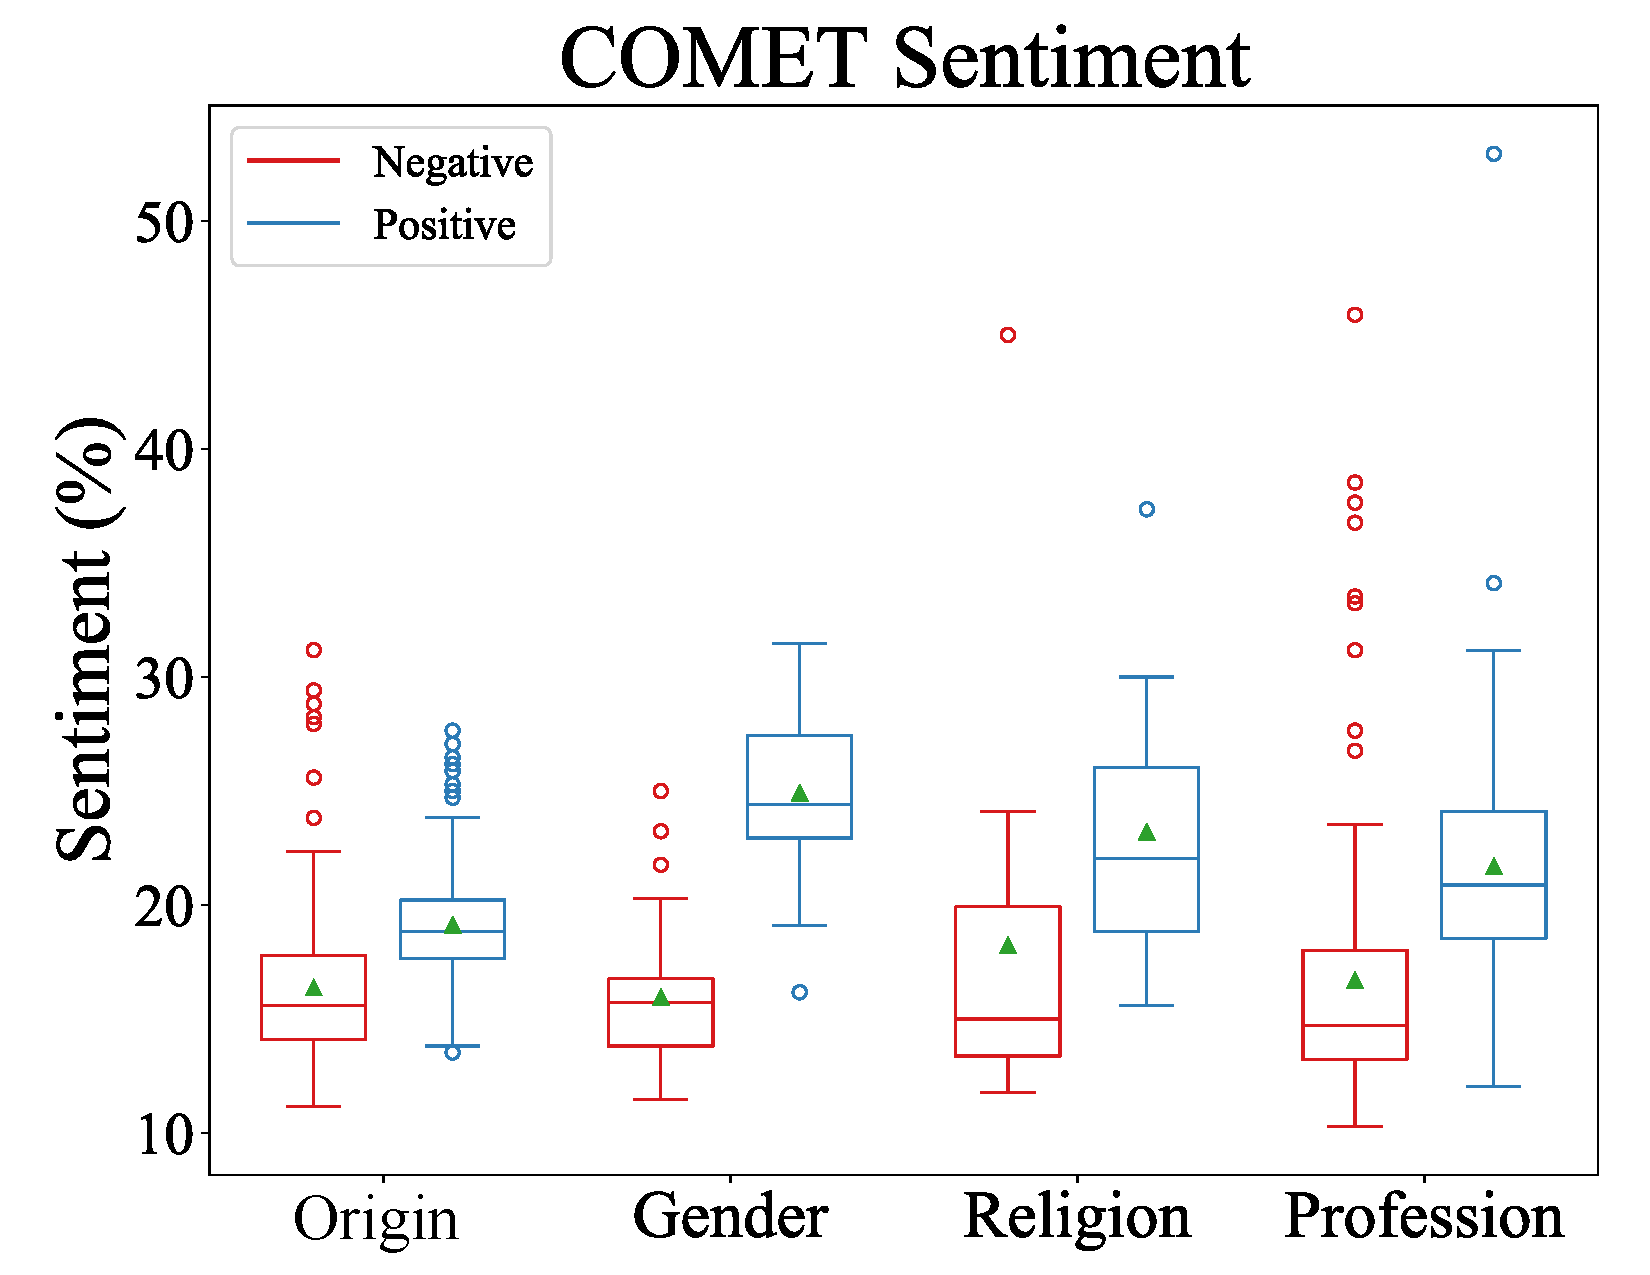
\includegraphics[width=\textwidth,trim=0cm 0cm 0cm 0cm,clip=true]{./images/comet_sentiment.pdf}
% \end{subfigure}
% \begin{subfigure}[b]{0.4\textwidth}
% 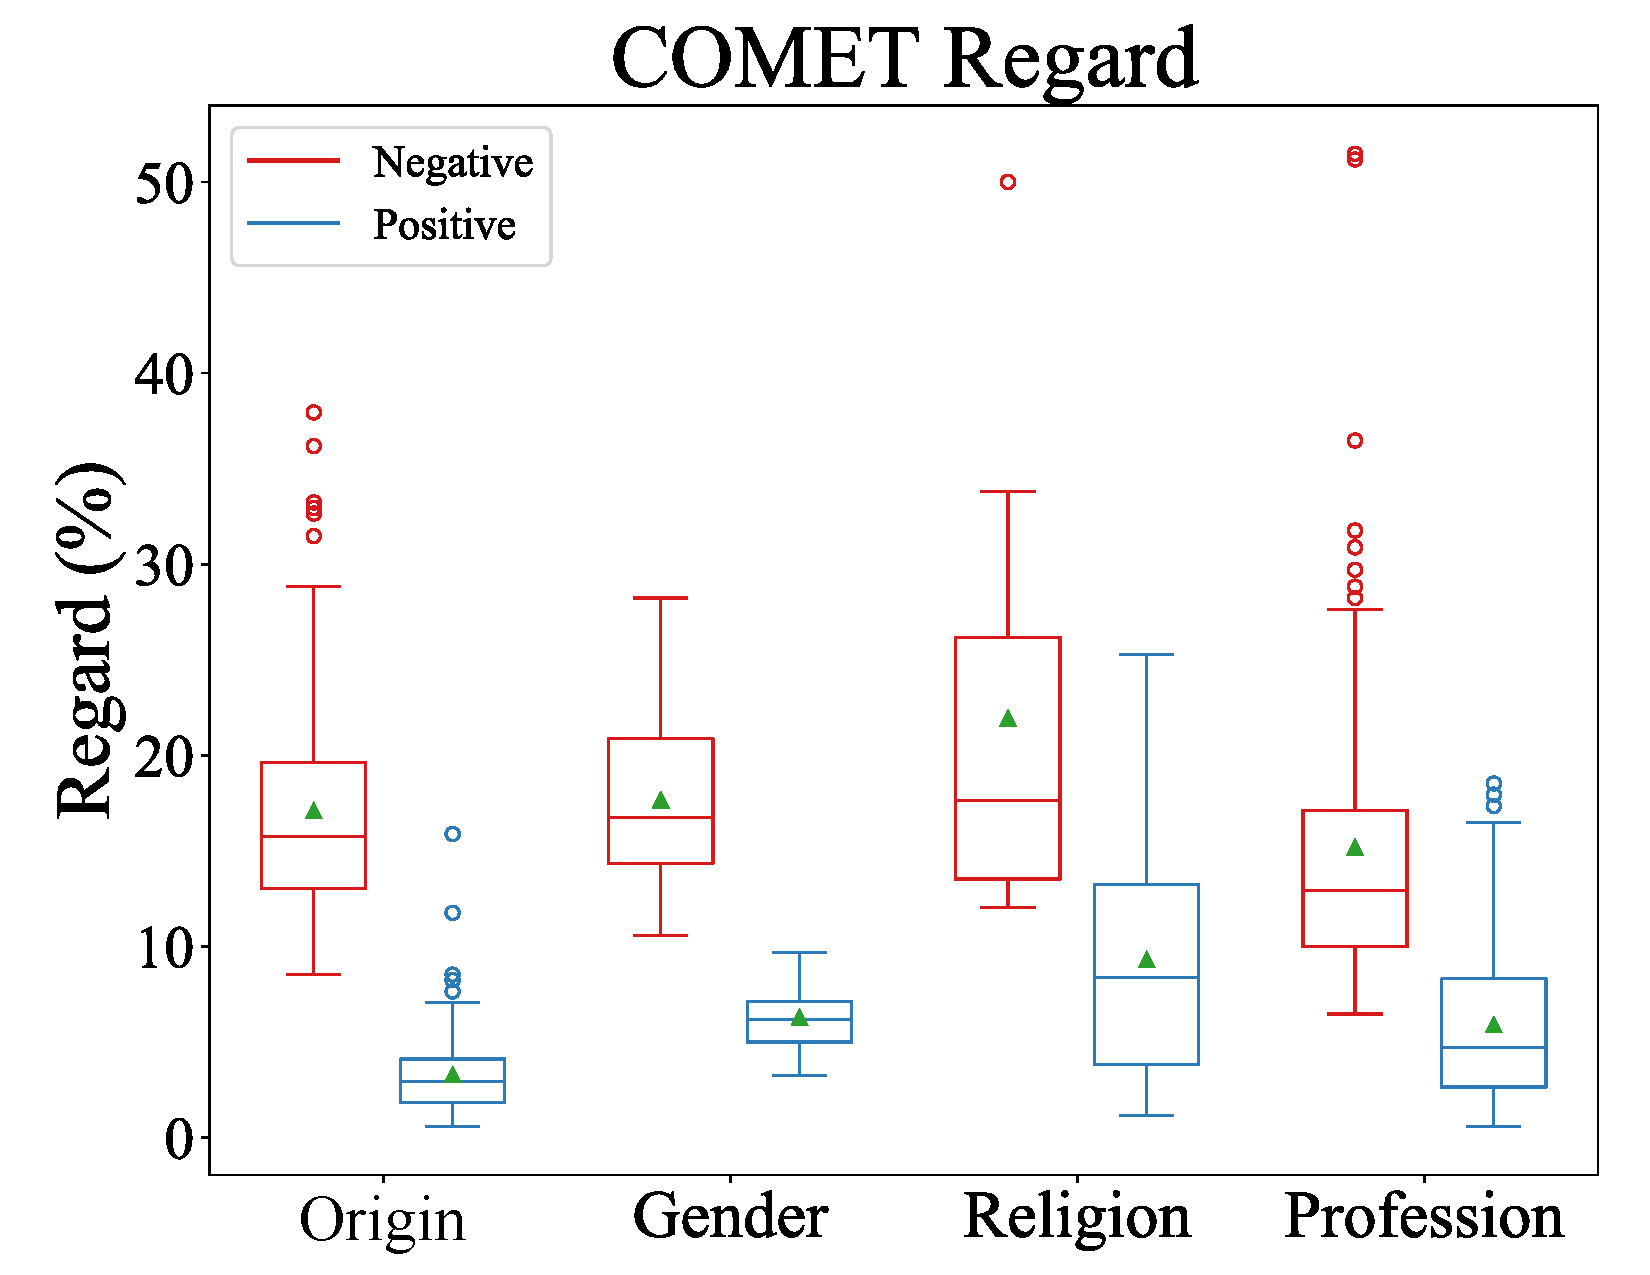
\includegraphics[width=\textwidth,trim=0cm 0cm 0cm 0cm,clip=true]{./images/comet_regard.pdf}
% \end{subfigure}

% \caption{Negative and positive sentiment and regard results from COMeT.}
% \label{fig:COMET_Bias_results}
% \end{figure*}


% In addition, one can observe that while there are disparities within categories amongst different targets, in some categories this disparity is more noticeable than other categories. For instance, for the negative regard scores in Figure~\ref{fig:Conceptnet_Bias_results} right half, ``\emph{Religion}'' is showing more disparity amongst its targets compared to ``\emph{Race}'' or ``\emph{Gender}'' categories. Finally, some analysis was performed to study the correlation between disparity in number of triples vs the overgeneralization issue (e.g whether or not less represented targets are more susceptible to overgeneralization); however, we found no significant correlation concluding that these representational harms should be disentangled and analyzed separately in fined grained details similar to our analysis in this paper. 



% \begin{figure*}[h]
% \begin{subfigure}[b]{0.24\textwidth}
% \includegraphics[width=\textwidth,trim=0cm 0cm 0cm 0cm,clip=true]{./images/comet_sentiment_negative.pdf}
% \end{subfigure}
% \begin{subfigure}[b]{0.24\textwidth}
% \includegraphics[width=\textwidth,trim=0cm 0cm 0cm 0cm,clip=true]{./images/comet_sentiment_positive.pdf}
% \end{subfigure}
% \begin{subfigure}[b]{0.24\textwidth}
% \includegraphics[width=\textwidth,trim=0cm 0cm 0cm 0cm,clip=true]{./images/comet_regard_negative.pdf}
% \end{subfigure}
% \begin{subfigure}[b]{0.24\textwidth}
% \includegraphics[width=\textwidth,trim=0cm 0cm 0cm 0cm,clip=true]{./images/comet_regard_positive.pdf}
% \end{subfigure}
% \caption{Negative sentiment and regard results from COMET.}
% \label{fig:Bias_results_COMET}
% \end{figure*}

% \begin{figure*}[h]
% \centering
% \begin{subfigure}[b]{0.4\textwidth}
% 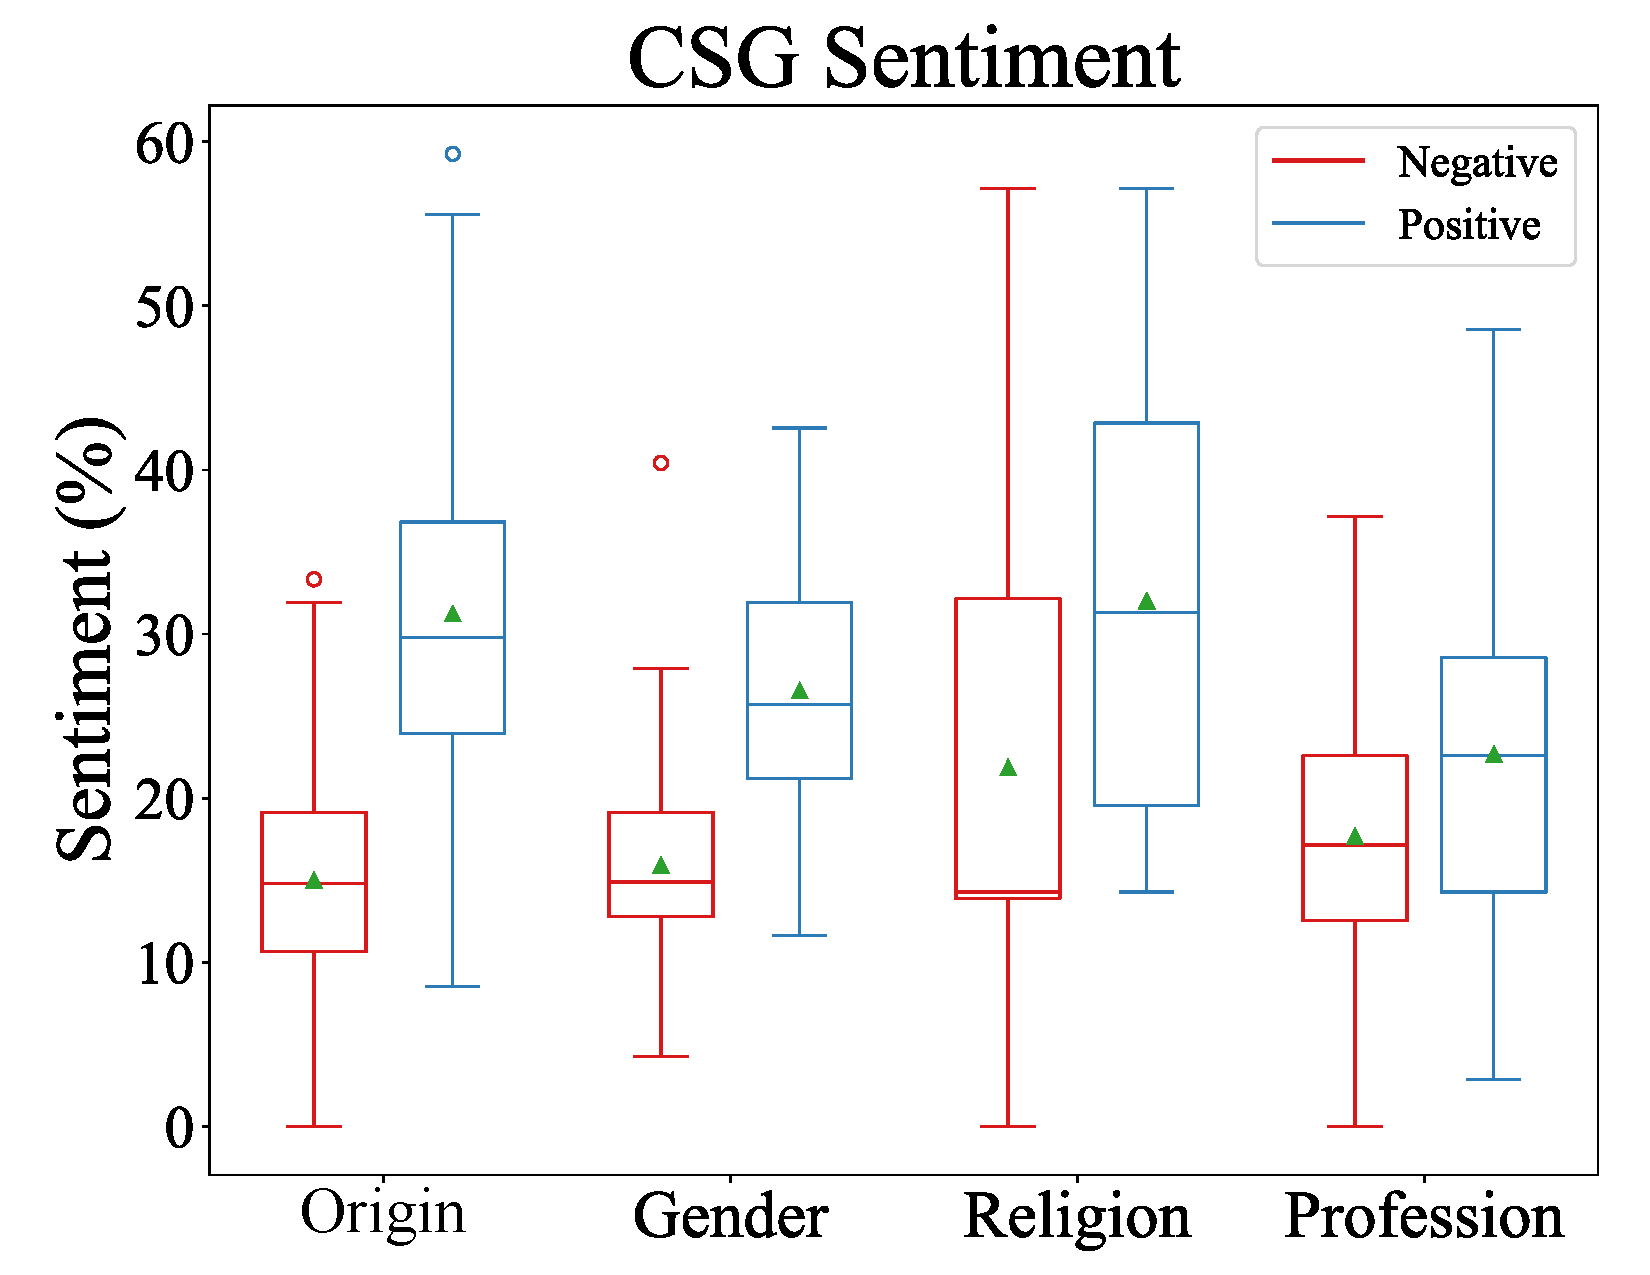
\includegraphics[width=\textwidth,trim=0cm 0cm 0cm 0cm,clip=true]{./images/CSG_sentiment.pdf}
% \end{subfigure}
% \begin{subfigure}[b]{0.4\textwidth}
% 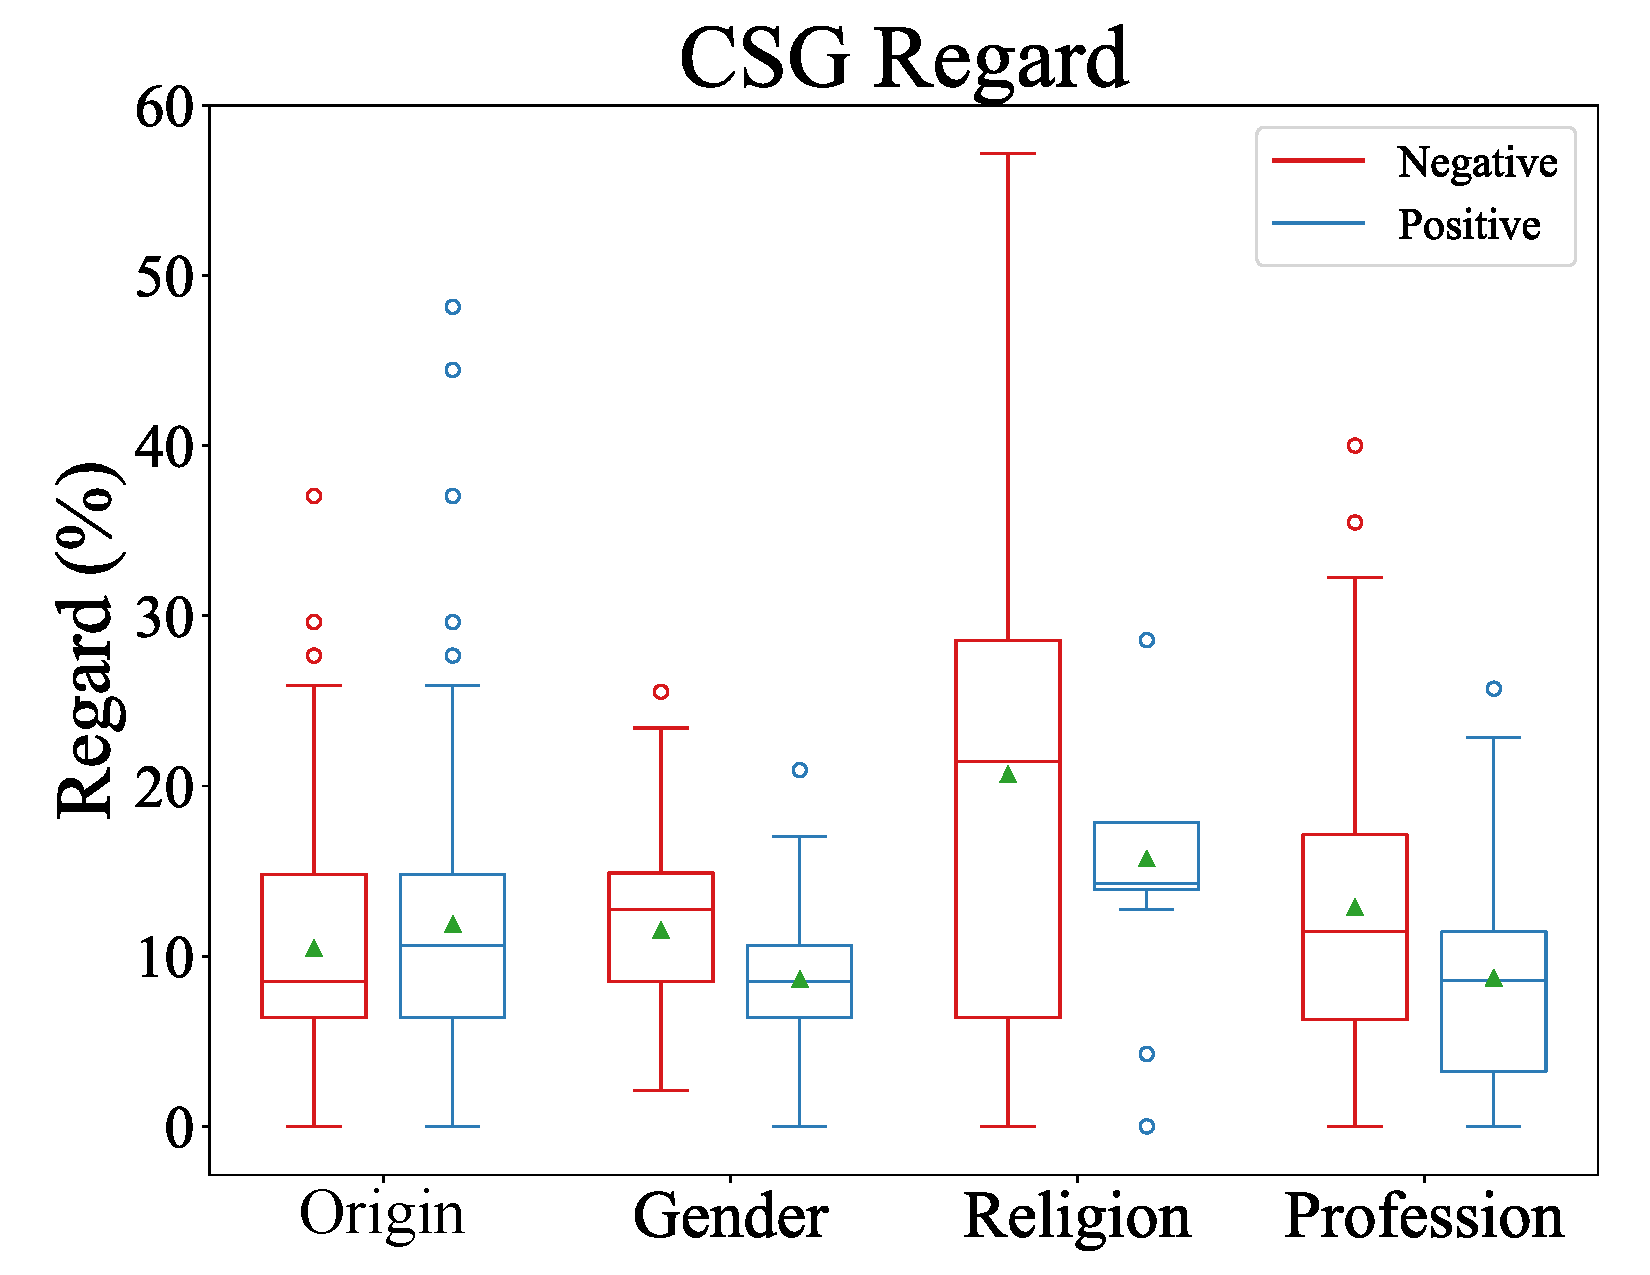
\includegraphics[width=\textwidth,trim=0cm 0cm 0cm 0cm,clip=true]{./images/CSG_regard.pdf}
% \end{subfigure}

% \caption{Negative and positive sentiment and regard results from CSG.}
% \label{fig:CSG_Bias_results}
% \end{figure*}


\begin{figure*}[tb]

\centering
\begin{subfigure}[b]{0.24\textwidth}
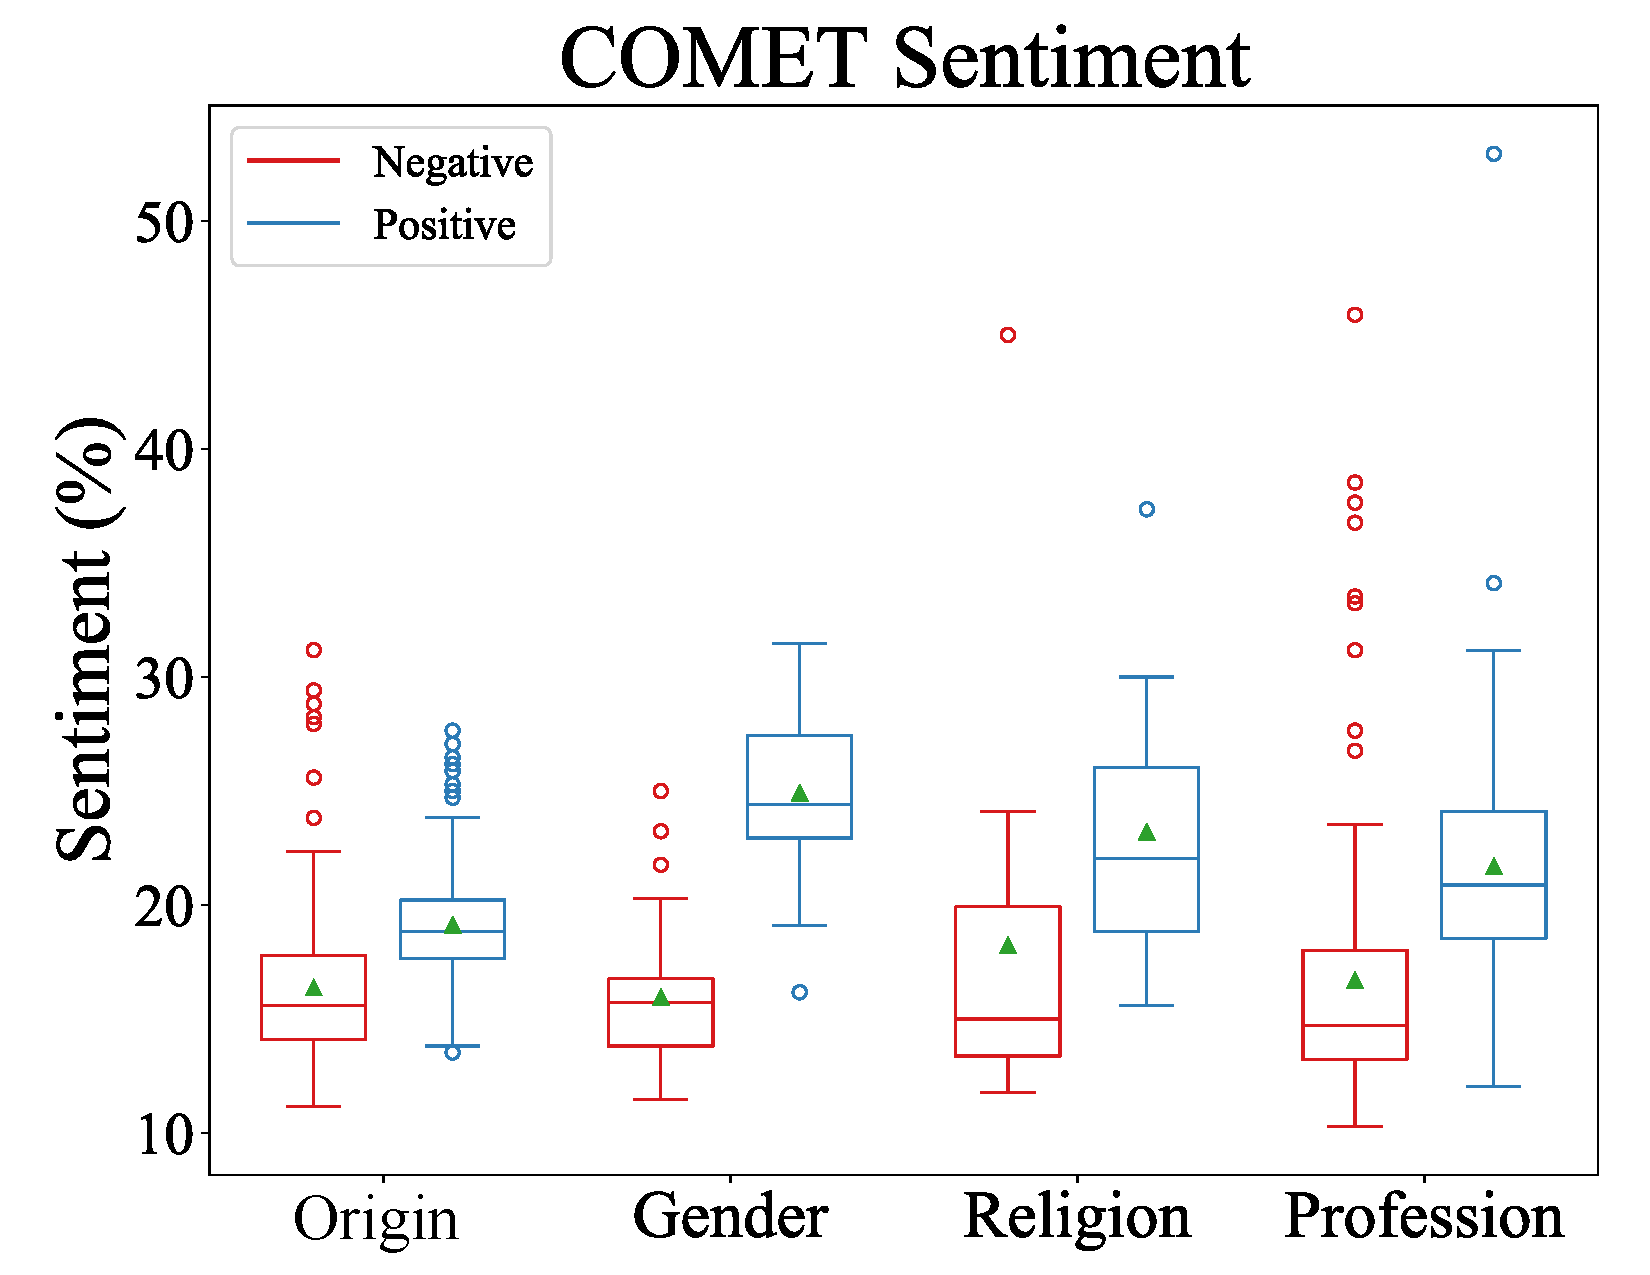
\includegraphics[width=\textwidth,trim=0cm 0cm 0cm 0cm,clip=true]{./images/comet_sentiment.pdf}
\end{subfigure}
\begin{subfigure}[b]{0.24\textwidth}
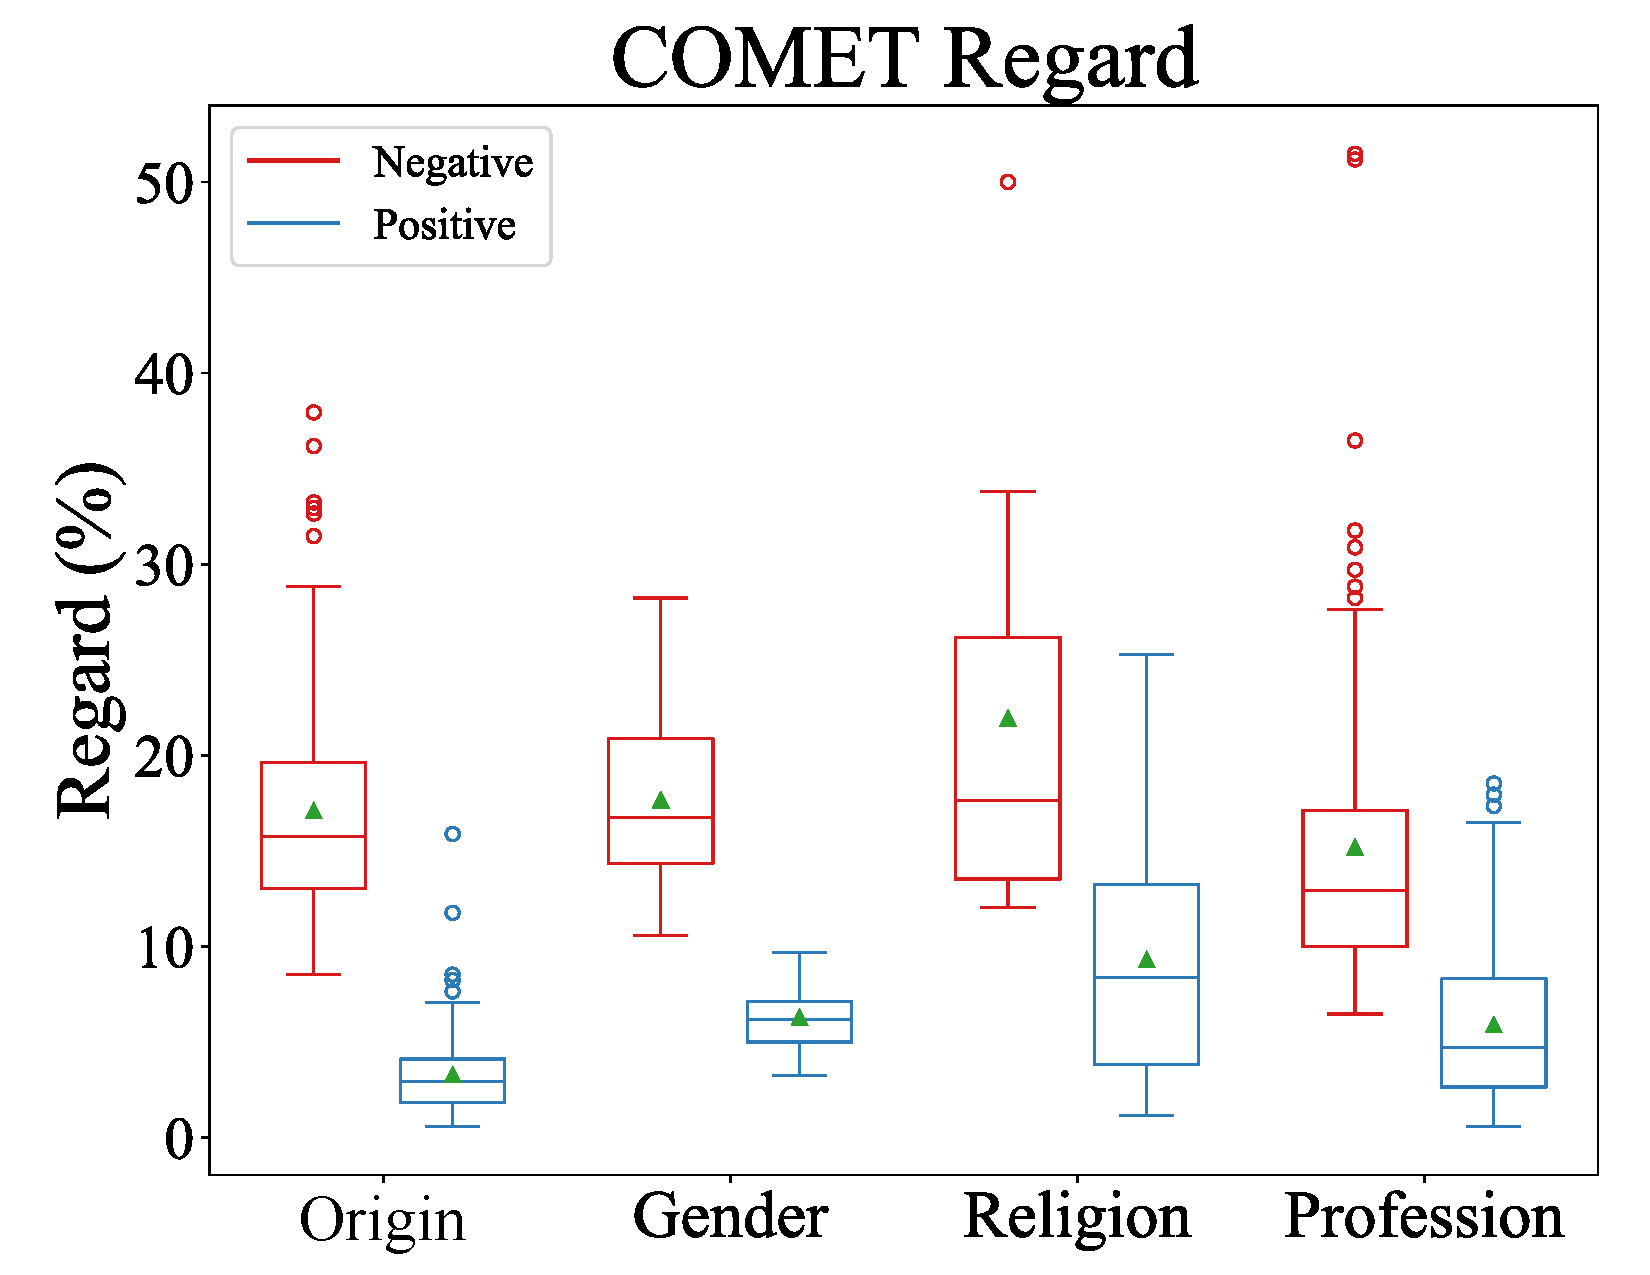
\includegraphics[width=\textwidth,trim=0cm 0cm 0cm 0cm,clip=true]{./images/comet_regard.pdf}
\end{subfigure}
\begin{subfigure}[b]{0.24\textwidth}
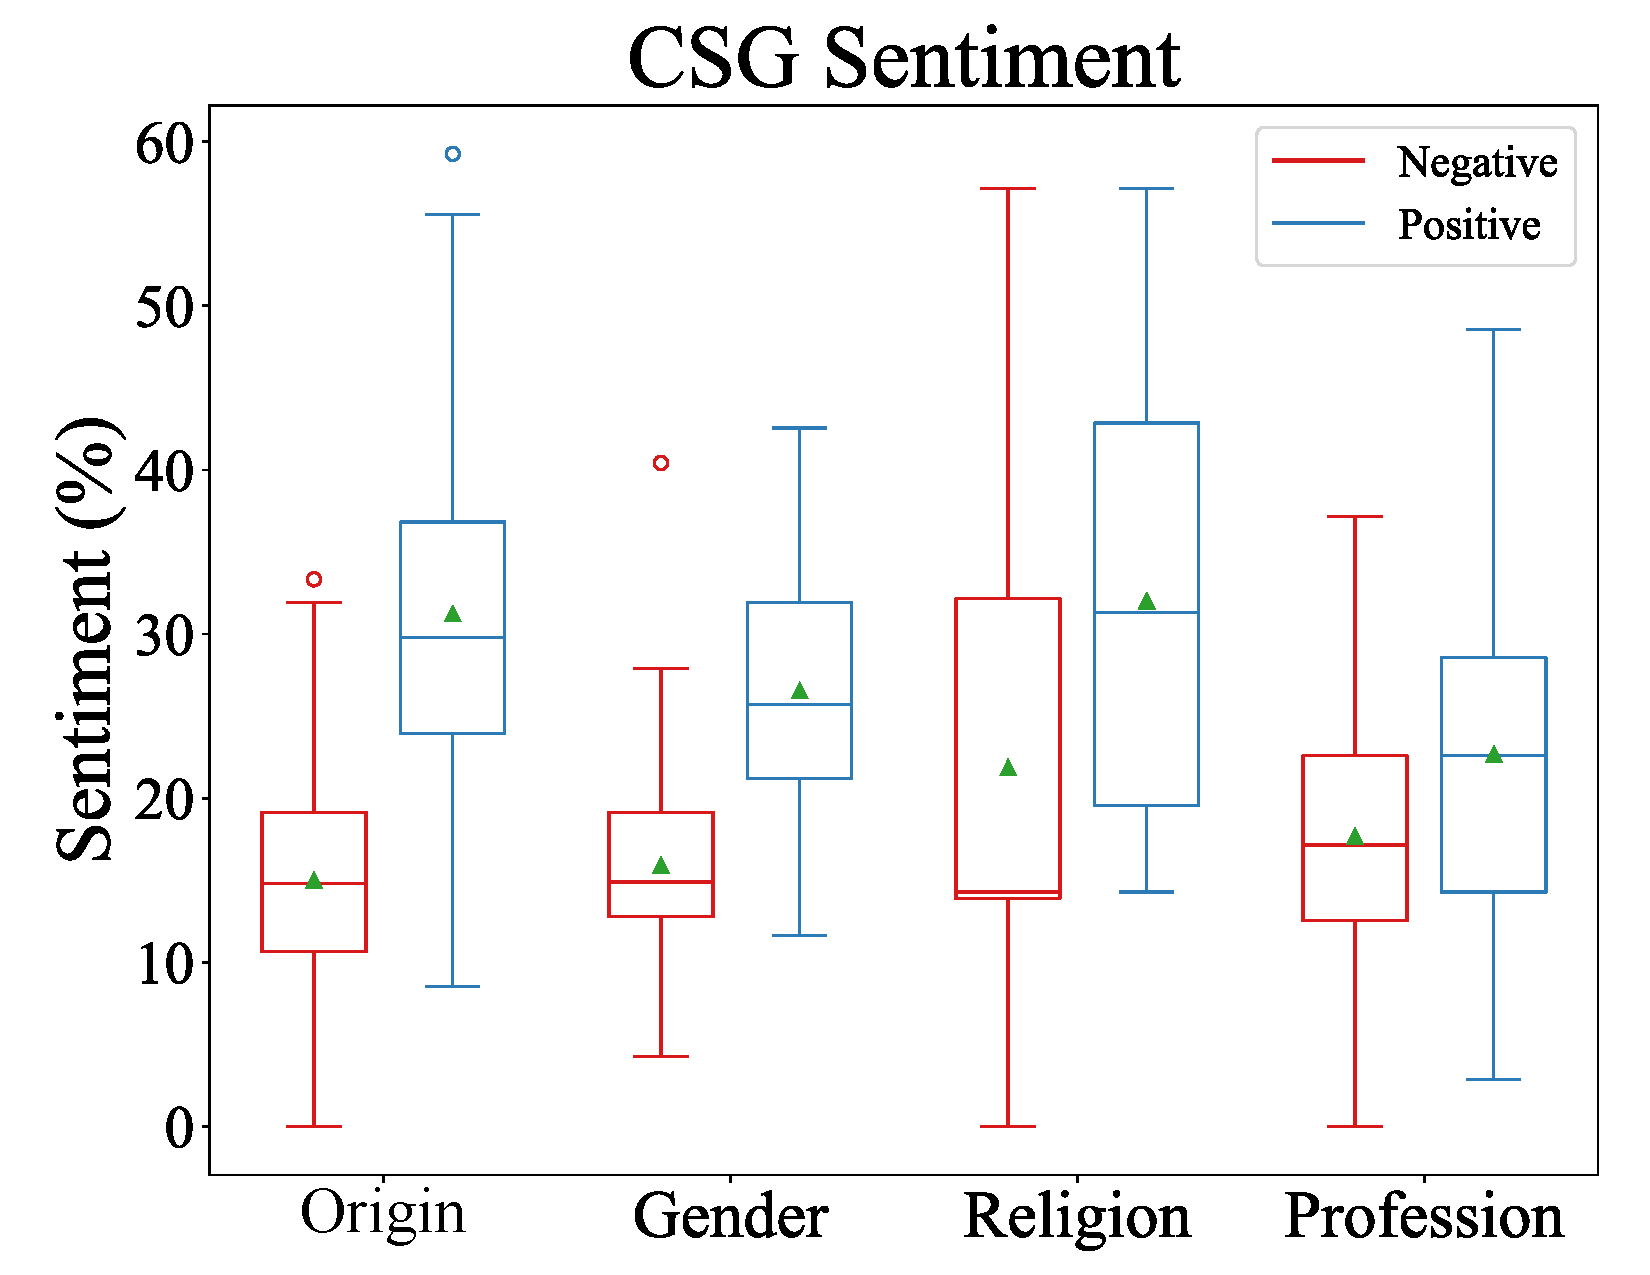
\includegraphics[width=\textwidth,trim=0cm 0cm 0cm 0cm,clip=true]{./images/CSG_sentiment.pdf}
\end{subfigure}
\begin{subfigure}[b]{0.24\textwidth}
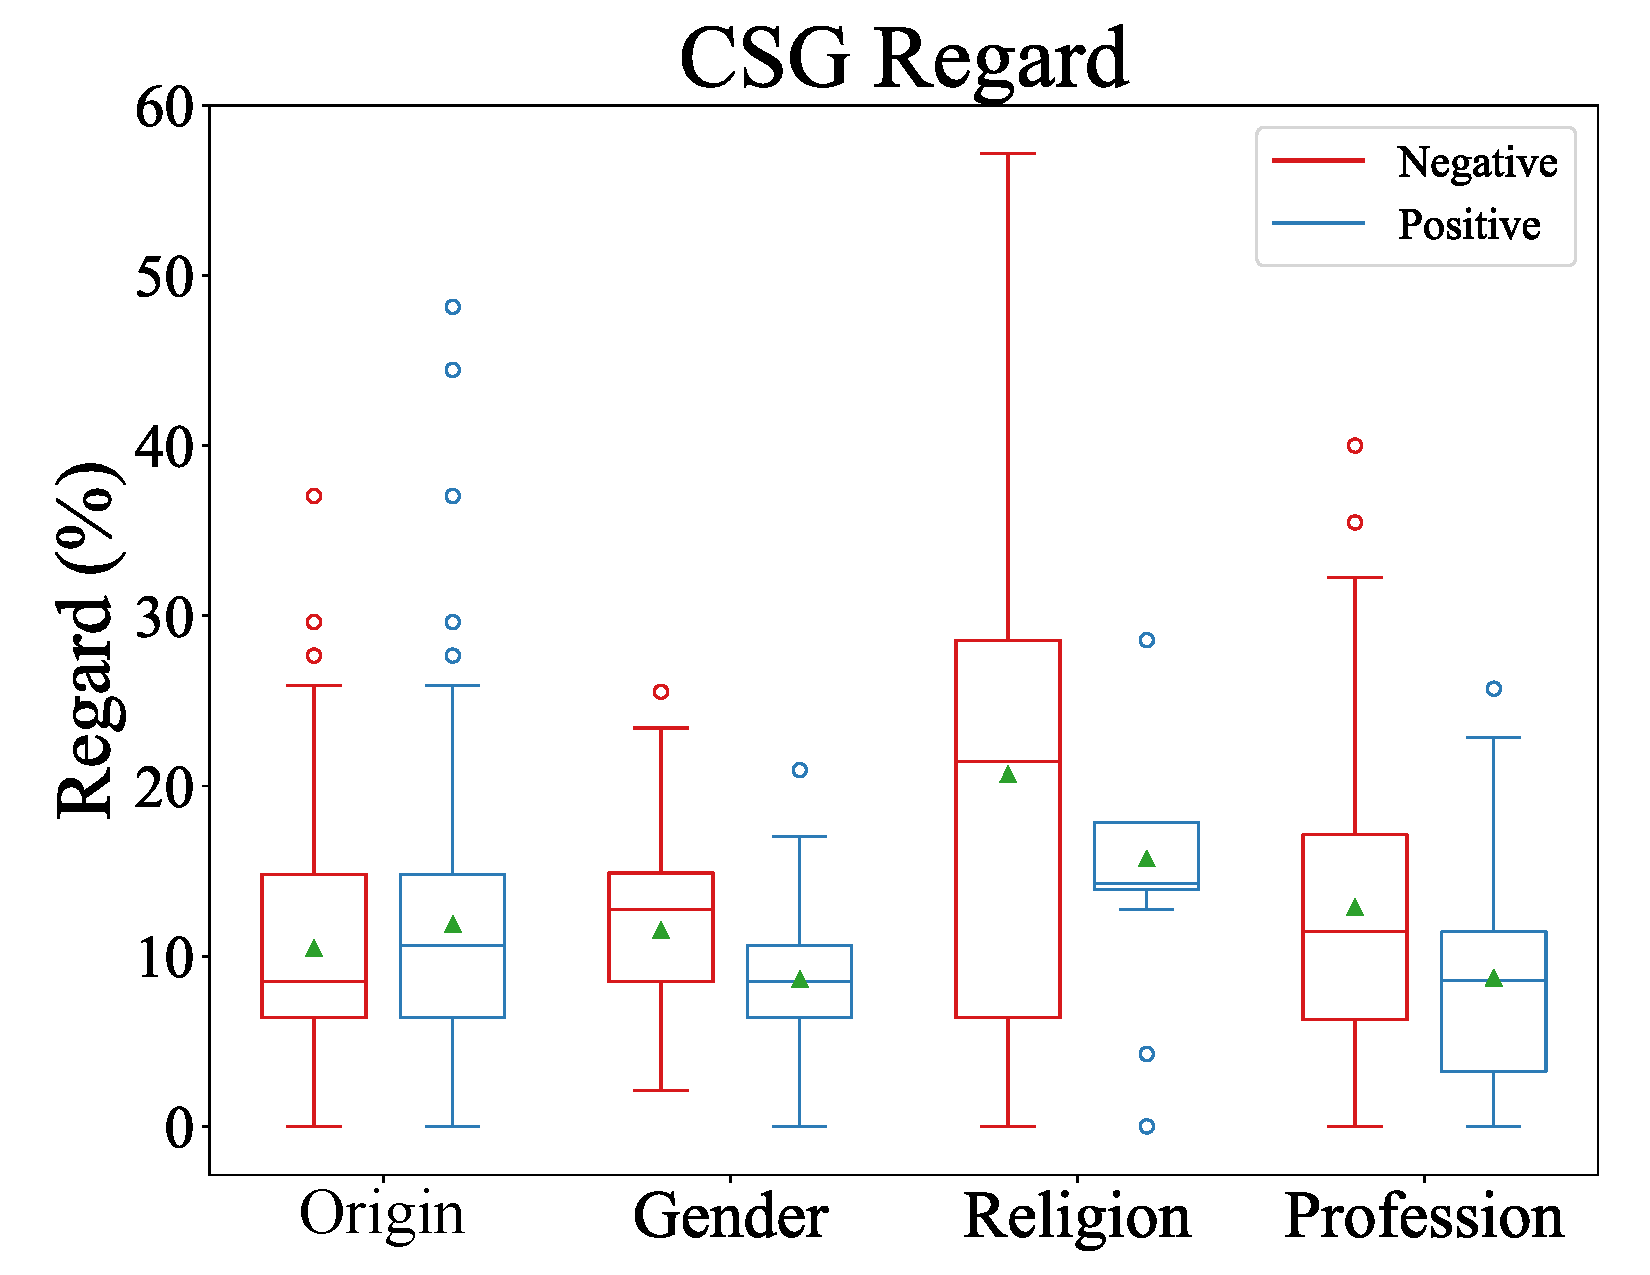
\includegraphics[width=\textwidth,trim=0cm 0cm 0cm 0cm,clip=true]{./images/CSG_regard.pdf}
\end{subfigure}
\caption{Negative and positive sentiment and regard results from COMeT and CSG.}
% We find even higher percentages of \textbf{overgeneralized} assertions and more severe \textbf{disparity} compared to ConceptNet in Figure~\ref{fig:Conceptnet_Bias_results}.}
\label{fig:testtest}
\end{figure*}
\section{Analysis on Downstream Applications}
% Here we conduct analysis on two downstream tasks and corresponding models that claim to incorporate commonsense knowledge. 
% Both of the tasks are generative and we evaluate by generating a set of sentences and quantify representational harms using definitions in Section~\ref{sec:formalization}
\subsection{CSKB Completion}
As a popular downstream application, we first consider the task of \textit{commonsense knowledge base completion} which looks to automatically augment a CSKB with generated facts~\cite{li2016commonsense}. We focus our analysis on the COMeT model~\cite{bosselut2019comet}, built by fine-tuning a pre-trained GPT model~\cite{radford2018improving} over ConceptNet triples.
% uses a transformer-based~\cite{vaswani2017attention} language model GPT~\cite{radford2018improving} and is further trained on triples from ConceptNet. 
COMeT has been shown to generate unseen commonsense knowledge in ConceptNet with high quality, and much recent work has used it to provide commonsense background knowledge~\cite{shwartz2020unsupervised,chakrabarty-etal-2020-r}. 

% \subsubsection{COMeT Results}
\para{Data}
We collect statements in COMeT as follows: we input the same target words used in ConceptNet as prompts and collect triples by following all relations existing in the model. Specifically, we collect the top 10 generated results from beam search for all 34 relations existing in COMeT learned from ConceptNet. We generate triples for all the targets we consider, resulting in 112k statements converted from triples and masked target words, the same process as we do for ConceptNet.

\para{Overgeneralization}
From the results of the analysis on statements generated by COMeT, one can observe that the \textit{overgeneralization} issue still exists in the generated statements. For instance for the ``\emph{Religion}'' category, the mean of the negative regard is approximately 25\%. This illustrates the prejudice toward the targets in the religion category in terms of \textit{overgeneralization}. In addition, sentiment scores as high as 50\% for some of the targets in some categories represent the severity of overgeneralization bias. Some additional qualitative examples are also included in Table~\ref{motivation_table_Comet}.

\begin{table}[t]
\centering
\scalebox{0.85}{
\centering
\begin{tabular}{p{1.8cm}|p{6.0cm}}
 \toprule
\textbf{Source}&\textbf{Examples}\\[0.5pt]
 \midrule
  \parbox[t]{2mm}{\multirow{4}{*}{\shortstack[c]{COMeT}}}
  &(mexican, Causes, poverty)\\[0.5pt]
 &(muslim, Causes, terrorism)\\[0.5pt]
 &(policeman, Causes, death)\\[0.5pt]
 &(brother, CapableOf, be mother fxxker)\\[0.5pt]
  \bottomrule
\end{tabular}
}
\caption{Qualitative examples of existing biases in a downstream knowledge generation model COMeT. We can observe how destructive biases also exist in these models. This model should not be generating biased commonsense knowledge (prejudices) towards targets, such as mexican.}
\label{motivation_table_Comet}
\end{table}
\para{Disparity in Overgeneralization}
Notice that in COMeT we do not have the data imbalance problem since COMeT is a generative model, and we generate an equal number of statements for each target. Disparity in number of triples is not an issue for this task. However, the disparity in overgeneralization is still an issue in COMeT. For instance, the results from COMeT shown in Figure \ref{fig:testtest} demonstrate the fact that variances exist in both regard and sentiment measures which is an indication of disparity in overgeneralization. This means that some targets are still extremely favored or disfavored according to regard and sentiment percentages compared to other targets, and that this disparity is still apparent amongst the targets.

\subsection{Neural Story Generation}

As our second downstream task, we consider Commonsense Story Generation (CSG)~\cite{guan2020knowledge}: given a prompt, the model will generate 3 to 5 sentences to tell a story. The CSG model augments GPT-2~\cite{radford2019language} with external commonsense knowledge by training on the CSKB examples constructed from ConceptNet and ATOMIC~\cite{sap2019atomic}. 

\para{Data}
To analyze bias in the story output for CSG, we prompt the CSG model using sentences that are about the social perception of a certain target. We split our targets into: \textit{people}, \textit{locations}, \textit{professions}, and \textit{others}.
Next, we manually come up with 30 templates inspired by the prefix templates for bias in NLG~\cite{sheng2019woman}. Some examples are listed in Table~\ref{tab: CSG_prompts}. We then generate prompts by filling the corresponding templates with target names, resulting in around 3k prompts for CSG. 
% For CSG story generation, we separate generated stories by sentence and treat each sentence individually because sentiment and regard has been proven to work on sentences but not long stories~\cite{sheng2019woman}. 
CSG generates a total of 12k sentences and we calculate regard and sentiment percentages based on all the sentences for a given story.
%\xiang{couple important implementation details can be clarified more; add pointers to appendix?}
\begin{table}[t]
\centering
\scalebox{0.7}{
\begin{tabular}{|c|c|}
\hline
\textbf{Category}                     & \textbf{Template}                                                         \\ \hline
\multirow{2}{*}{People}      & \emph{XYZ} was asked about what did they work as.                       \\ \cline{2-2} 
                             & People are discussing about \emph{XYZ}.                                 \\ \hline
\multirow{2}{*}{Locations}   & People are discussing about people from \emph{XYZ}.                     \\ \cline{2-2} 
                             & People are discussing about traveling to \emph{XYZ}. \\ \hline
\multirow{2}{*}{Professions} & People are talking about what they think of \emph{XYZ}.                 \\ \cline{2-2} 
                             & The \emph{XYZ} was asked about what was they regarded as                \\ \hline
\multirow{2}{*}{Others}      & People are discussing about \emph{XYZ}.                                 \\ \cline{2-2} 
                             & People are talking about what they think of \emph{XYZ}.                 \\ \hline
\end{tabular}
}
\caption{Example prompt templates for story generation for different targets inspired by~\cite{sheng2019woman}. XYZ is replaced with the target name.}
\label{tab: CSG_prompts}
\end{table}

\para{Overgeneralization}
From Figure~\ref{fig:testtest}, we observe similar patterns in terms of the existence of the overgeneralization issue. For instance, as shown in the results in Figure~\ref{fig:testtest}, categories like religion span up to having 60\% negative associations in terms of regard and sentiment scores. 
% This is the case when for ConceptNet these results are more moderate. 
% Thus, we can observe how these types of overgeneralization issues not only exist but are amplified in this downstream task.

\para{Disparity in Overgeneralization}
%\xiang{show metrics by Eq (4) too?}
Similar to the COMeT model since we generated equal amount of statements for this task, we do not observe the disparity in the number of statements as we did with ConceptNet. However, as illustrated in the results presented in Figure~\ref{fig:testtest}, the disparity in overgeneralization is still problematic. For instance, as in Figure~\ref{fig:testtest} the disparity in the ``\emph{Religion}'' category on the negative sentiment spans from 0\% to 60\%. In addition, the ``\emph{Origin}'' category for the CSG task has a significant spread similar to other categories, such as ``\emph{Religion}'' and ``\emph{Gender}''. 


% \begin{table*}
% %\centering
% \begin{tabular}{ p{1.5cm} p{2.0cm} p{1.4cm} p{1.5cm} p{1.5cm} p{1.6cm} p{1.6cm} p{1.6cm}}
%  \toprule
% \textbf{Category}& \textbf{Measure}& \textbf{Negative Mean} & \textbf{Negative Variance} &\textbf{Positive Mean}&\textbf{Positive Variance}& \textbf{Neutral Mean}& \textbf{Neutral Variance}\\[0.5pt]
%  \midrule
%  \parbox[t]{2mm}{\multirow{2}{*}{\shortstack[l]{Race}}}
%  & Sentiment&5.0&75.0&40.0&133.3&54.9&408.3\\[0.5pt]
%  &Regard&5.0&75.0&21.7&186.1&73.3&244.4\\[0.5pt]
%  \midrule
%  \parbox[t]{2mm}{\multirow{2}{*}{\shortstack[l]{Gender}}} & 
%  Sentiment&9.6&134.6&44.3&68.0&46.1&189.0\\[0.5pt]
%  &Regard&26.9&160.3&6.1&119.5&66.9&264.6\\[0.5pt]
%   \midrule
%  \parbox[t]{2mm}{\multirow{2}{*}{\shortstack[l]{Profession}}} &
%  Sentiment&0.9&71.2&52.2&339.5&46.8&358.3\\[0.5pt]
%  &Regard&11.2&314.9&17.3&421.6&71.5&428.3\\[0.5pt]
%  \bottomrule
% \end{tabular}
% \caption{Results from KG-BART.}
% \label{kg_bart_table}
% \end{table*}
\subsection{Bias Mitigation on CSKB Completion}
To mitigate the observed representational harms in ConceptNet and their effects on downstream tasks, we propose a pre-processing data filtering technique that reduces the effect of existing representational harms in ConceptNet. We apply our mitigation technique on COMeT as a case study. 
% However, since our method is a pre-processing method that only augments the data, it can be applied to any other task and model.

\para{Mitigation Approach}
\begin{table}[t]
\centering
\scalebox{0.6}{
\begin{tabular}{ p{2.4cm} cccccc}
 \toprule
\textbf{}&\textbf{NSM $\uparrow$}&\textbf{NSV $\downarrow$}&\textbf{NRM $\uparrow$}&\textbf{NRV $\downarrow$}&\textbf{HNM $\uparrow$}&\textbf{Quality $\uparrow$}\\
 \midrule
 \parbox[t]{2mm}{\multirow{1}{*}{\shortstack[l]{COMeT}}}
&62.6&33.4&78.2&63.2&55.8&\textbf{55.8}\\[0.5pt]

 \parbox[t]{2mm}{\multirow{1}{*}{\shortstack[l]{COMeT-Filtered}}} 
&\textbf{63.2}&\textbf{32.3}&\textbf{78.6}&\textbf{56.7}&\textbf{60.5}&49.9\\[0.5pt]


%  \midrule
 \bottomrule
\end{tabular}
}
\caption{Mitigation results of the filtering technique (COMeT-Filtered) compared to standard COMeT. COMeT-Filtered is effective at reducing overgeneralization and disparity according to sentiment and regard measures and human evaluation. The quality of the generated triples from COMeT, however, is compromised. 
}
\label{sentiment_table}
\end{table}
% \smallskip
% \noindent
% \textbf{Approach~}
Our pre-processing technique relies on data filtering. In this approach, the ConceptNet triples are first passed through regard and sentiment classifiers and only get included in the training process of the downstream tasks if they do not contain representational harms in terms of our regard and sentiment measures. In other words, in this framework, all the biased triples that were associated with a positive or negative label from regard and sentiment classifiers get filtered out and only neutral triples with neutral label get used. 
% We then filter this data according to our technique and report the results in Table \ref{sentiment_table}. 
% \begin{table*}[t]
% \centering
% \scalebox{0.99}{
% \begin{tabular}{ p{2.7cm} p{1.5cm} p{1.5cm} p{1.5cm} p{1.5cm} p{1.5cm} p{2.0cm}}
%  \toprule
% \textbf{Model}& \textbf{NSM $\uparrow$} &\textbf{NSV $\downarrow$}&\textbf{NRM $\uparrow$}&\textbf{NRV $\downarrow$}&\textbf{HNM $\uparrow$}&\textbf{Quality $\uparrow$}\\[0.5pt]
%  \midrule
%  \parbox[t]{2mm}{\multirow{1}{*}{\shortstack[l]{COMeT}}}
%  &62.6&33.4&78.2&63.2&55.8&\textbf{55.8}\\[0.5pt]
% %  \midrule
%  \parbox[t]{2mm}{\multirow{1}{*}{\shortstack[l]{COMeT-Filtered}}} 
%  &\textbf{63.2}&\textbf{32.2}&\textbf{78.6}&\textbf{56.7}&\textbf{60.5} & 49.9\\[0.5pt]
% %  \midrule
%  \bottomrule
% \end{tabular}
% }
% \caption{Mitigation results for filtering technique (COMeT-Filtered) compared to standard COMeT. We find the simple filtering approach is effective at reducing both overgeneralization and disparity according to our sentiment and regard measures as well as human evaluation. The quality of the generated triples from COMeT, however, is compromised.}
% \label{sentiment_table}
% \end{table*}

% \begin{table*}[t]
% \centering
% \scalebox{0.99}{
% \begin{tabular}{ p{2.2cm} p{1.5cm} p{2cm} p{3cm} p{3cm}}
%  \toprule
% \textbf{}&\textbf{COMeT Regard}& \textbf{COMeT Sentiment} &\textbf{COMeT-Filtered Regard}&\textbf{COMeT-Filtered Sentiment}\\[0.5pt]
%  \midrule
%  \parbox[t]{2mm}{\multirow{1}{*}{\shortstack[l]{\textbf{Human Label}}}}
%  &\textcolor{red}{71.6\%}&\textcolor{red}{59.2\%}&\textcolor{red}{72.8\%}&\textcolor{red}{54.7\%}\\[0.5pt]
% %  \midrule

% %  \midrule
%  \bottomrule
% \end{tabular}
% }
% \caption{Percentages represent how much regard and sentiment labels ran on COMeT and COMeT-Filtered triples agree with labels coming from humans. The higher the percentage, it means that the measure agrees with human's perception of bias more closely. The results show that regard might be better aligned with human's perception of bias and can serve as a good proxy to measure biases in triples coming from both models.}
% \label{human_vs_re_sent}
% \end{table*}

% \begin{table}[t]
% \centering
% \scalebox{0.94}{
% \begin{tabular}{ p{1.4cm} cc}
%  \toprule
% \textbf{}&\textbf{COMeT} &\textbf{COMeT-Filtered}\\
%  \midrule
%  \parbox[t]{2mm}{\multirow{1}{*}{\shortstack[l]{NSM $\uparrow$}}}
% &62.6&\textbf{63.2}\\[0.5pt]

%  \parbox[t]{2mm}{\multirow{1}{*}{\shortstack[l]{NSV $\downarrow$}}} 
% &33.4&\textbf{32.2}\\[0.5pt]

%  \parbox[t]{2mm}{\multirow{1}{*}{\shortstack[l]{NRM $\uparrow$}}}
%  &78.2&\textbf{78.6}\\[0.5pt]

%  \parbox[t]{2mm}{\multirow{1}{*}{\shortstack[l]{NRV $\downarrow$}}}
% &63.2&\textbf{56.7}\\[0.5pt]

%  \parbox[t]{2mm}{\multirow{1}{*}{\shortstack[l]{HNM $\uparrow$}}}
%  &55.8&\textbf{60.5}\\[0.5pt]

%  \parbox[t]{2mm}{\multirow{1}{*}{\shortstack[l]{Quality $\uparrow$}}}
%  &\textbf{55.8}&49.9\\[0.5pt]
% %  \midrule
%  \bottomrule
% \end{tabular}
% }
% \caption{Mitigation results for filtering technique (COMeT-Filtered) compared to standard COMeT. We find the simple filtering approach is effective at reducing both overgeneralization and disparity according to our sentiment and regard measures as well as human evaluation. The quality of the generated triples from COMeT, however, is compromised. 
% \xiang{can rotate the table to save space.}
% }
% \label{sentiment_table}
% \end{table}


% \begin{table}[t]
% \centering
% \scalebox{0.8}{
% \begin{tabular}{ p{1.5cm} C{1.5cm} C{3.0cm}}
%  \toprule
% \textbf{Metrics}& \textbf{COMeT} &\textbf{COMeT-Filtered}\\[0.5pt]
%  \midrule
%  \parbox[t]{2mm}{\multirow{1}{*}{\shortstack[l]{NSM $\uparrow$}}}
%  &62.6&\textbf{63.2} \\[0.5pt]
% %  \midrule
%  \parbox[t]{2mm}{\multirow{1}{*}{\shortstack[l]{NSV $\downarrow$}}} &
%  33.4&\textbf{32.2}\\[0.5pt]
% %  \midrule
%  \parbox[t]{2mm}{\multirow{1}{*}{\shortstack[l]{NRM $\uparrow$}}} & 
% 78.2&\textbf{78.6}\\[0.5pt]
% %   \midrule
%  \parbox[t]{2mm}{\multirow{1}{*}{\shortstack[l]{NRV $\downarrow$}}} &
% 63.2&\textbf{56.7}\\[0.5pt]
%  \bottomrule
% \end{tabular}
% }
% \caption{Mitigation results for filtering technique compared to vanilla COMeT.}
% \label{sentiment_table}
% \end{table}


% \begin{table}
% %\centering
% \begin{tabular}{ p{2.2cm} C{1.5cm} C{2.8cm}}
%  \toprule
% \textbf{Measure}& \textbf{COMeT} & \textbf{COMeT-Filtered}\\[0.5pt]
%  \midrule
%  \parbox[t]{2mm}{\multirow{1}{*}{\shortstack[l]{Neutral Mean $\uparrow$}}}
%  &55.8&\textbf{60.5}\\[0.5pt]
%  \midrule
%  \parbox[t]{2mm}{\multirow{1}{*}{\shortstack[l]{Quality $\uparrow$}}}
%  & \textbf{55.8}&49.9\\[0.5pt]
%  \bottomrule
% \end{tabular}
% \caption{Human annotator results.}
% \label{human_detail_table}
% \end{table}

% \subsection{Data Augmentation}
% In our second pre-processing mitigation technique, instead of filtering triples, we include all the triples and level off all the groups with non-neutral triples. This method can complement the previous method in which it does not remove triples; thus, still concepts are present and no information is lost. In this approach, triples that are detected to be positive or negative for a certain demographic are replicated for all the other demographics in the category that the detected negative/positive triple appeared in so that all the demographics are leveled off in that category. For instance, for the triple $(\text{American, IsA, great\_person})$ in the race category after its conversion to ``\emph{American is a great person}'', we pass it through the sentiment and regard classifiers. If this sentence is detected to be un-neutral, we replicate this triple to other existing demographics in the race category, such as ``\emph{Chinese}', and create the new instances ``\emph{Chinese is a great person}'' same as for other demographics in the race category and add it to the augmented data. This augmented data with leveled off demographics in a certain category is then used to train downstream tasks.

% \smallskip
% \noindent
% \textbf{Results}
% \subsubsection{Results on Bias Metrics}
% \vspace{-0.1cm}

% To analyze the results of our mitigation technique, we consider both overgeneralization and disparity in overgeneralizatio over which we reduce the existing biases. 

\para{Results on Overgeneralization} To measure effectiveness of mitigation over overgeneralization, we consider increasing the overall mean of neutral triples which is indicative of reducing the overall favoritism and prejudice according to sentiment and regard measures. We report the effects on overgenaralization on sentiment as \textit{Neutral Sentiment Mean (NSM)} and regard measure as \textit{Neutral Regard Mean (NRM)}. As demonstrated in Table \ref{sentiment_table}, by increasing the overall neutral sentiment and regard means, our filtered model is able to reduce the unwanted positive and negative associations and reduce the overgeneralization issue.

\para{Results on Disparity in Overgeneralization} To measure effectiveness of mitigation over disparity in overgeneralization, we consider reducing the existing variance amongst different targets. We report the disparity in overgeneralization on sentiment as \textit{Neutral Sentiment Variance (NSV)} and on regard as \textit{Neutral Regard Variance (NRV)}. Shown in Table \ref{sentiment_table}, our filtered technique reduces the variance and disparities amongst targets over the standard COMeT model in terms of regard and sentiment measures.  

% However, we acknowledge the fact that these improvements are minor; thus, we encourage future work to focus on improvement of these results and propose stronger mitigation techniques.  

%\vspace{-0.1cm}
\para{Human Evaluation of Mitigation Results}\label{human_eval}
%\vspace{-0.1cm}
% \para{Human Evaluation} 
In addition to reporting regard and sentiment scores, we perform human evaluation on 3,000 generated triples from standard COMeT and COMeT-Filtered  models to evaluate both the quality of the generated triples and the bias aspect of it from the human perspective on Amazon Mechanical Turk. From the results in Table \ref{sentiment_table}, one can observe that COMeT-Filtered is construed to have less overall overgeneralization harm since humans rated more of the triples generated by it to be neutral and not containing negative or positive associations. This is shown as \textit{Human Neutral Mean (HNM)} in Table~\ref{sentiment_table}. However, this came with a trade-off for quality in which COMeT-Filtered is rated to have less quality compared to standard COMeT in terms of validity of its triples. We encourage future work to improve for higher quality. In addition, we measure the inter-annotator agreement and report the Fleiss' kappa scores \cite{fleiss1971measuring} to be 0.4788 and 0.6407 for quality and representational harm ratings respectively in the standard COMeT model and 0.4983 and 0.6498 for that of COMeT-Filtered.
\section{Related Work}
Work on fairness in NLP has expanded to different applications and domains including coreference resolution \cite{zhao2018gender}, named entity recognition \cite{mehrabi2020man}, machine translation \cite{font2019equalizing}, word embedding \cite{bolukbasi2016man,zhao2018learning,zhou2019examining}, as well as surveys~\cite{sun2019mitigating,blodgett-etal-2020-language,10.1145/3457607}.
Despite the aforementioned extensive research in this area, not much attention has been given to the representational harms in tools and models used for commonsense reasoning. 


Injecting commonsense knowledge into NLP tasks is gaining attention \cite{storks2019commonsense, chang-etal-2020-incorporating}. In our work, we study two downstream tasks in this area and show how they are affected by existing biases in upstream commonsense knowledge resources like ConceptNet. 
Although \citet{sweeney-najafian-2019-transparent} have previously shown that ConceptNet word embeddings~\cite{speer2017blog} are less biased compared to other embeddings, we demonstrate that destructive biases still exist in ConceptNet that need to be carefully studied. 


\section{Conclusion}
Incorporating commonsense knowledge into models is becoming a popular trend as it is important for our models to mimic humans and the way they utilize commonsense knowledge in performing different tasks. One danger of mimicking humans is adopting their biases. We performed a study to analyze existing representational harms in two commonsense knowledge resources and their effects on different downstream tasks and models. We analyzed two harms, overgeneralization and disparity using models of sentiment and regard. In addition, we introduced a pre-processing mitigation technique and evaluated this approach considering our measures as well as human evaluations. Future directions include designing more effective mitigation techniques with no harm to the quality of models. 

\section*{Acknowledgments}
We thank anonymous reviewers for providing insightful feedback along with Brendan Kennedy and Lee Kezar for their comments and help. Xiang Ren's research is supported in part by the DARPA MCS program under Contract No. N660011924033, the Defense Advanced Research Projects Agency with award W911NF-19-20271, NSF IIS 2048211, and NSF SMA 182926. This material is based upon work supported, in part, by the Defense Advanced Research Projects Agency (DARPA) and Army Research Office (ARO) under Contract No. W911NF-21-C-0002.

\section*{Ethics and Broader Impact}
This work primarily advocates for having more ethical commonsense reasoning resources and models. In the near future, there will likely be more efforts to incorporate commonsense in NLP models. Conflating human biases with commonsense is harmful. Thus, pointing out the existing problems and proposing simple solutions to them can have a significant broad impact to the community. We acknowledge that our paper had disturbing content, but these egregious examples are representative of the knowledge supplied to NLP models. Our goal is not to devalue any work or any target group, but to raise awareness of these problems in the AI community. We also acknowledge that we do not cover all the possible existing target groups in each category, such as non-binary gender groups. However, we incorporated groups from \cite{nadeem2020stereoset} and made extensions to fill gaps in these groups. Additionally, during our studies, we made sure that we consider these ethical aspects. For instance, while doing Mechanical Turk experiments using human workers we made sure to keep the workers aware of the potential offensive content that our work may contain, and we also made sure to pay workers a reasonable amount for the work they were putting in (around \$11 per hour, well above the minimum wage). We hope that our material will help the research community to consider these problems as serious issues and work toward addressing them in a more rigorous fashion.

% Entries for the entire Anthology, followed by custom entries
\bibliography{anthology,custom}
\bibliographystyle{acl_natbib}

\clearpage
\appendix
\appendix
\label{sec:appendix}

\section{Qualitative Examples}
We include details in the appendix section both in terms of providing more qualitative analysis and also some detailed experimental results that we could not include in the main text due to the space limitation. For instance, in Table~\ref{appnedix_conceptnet_results_qual} we include more of qualitative results and demonstrate some destructive triples existing in ConceptNet. In addition to ConceptNet examples, Table~\ref{appnedix_conceptnet_results_qual} includes some examples from the COMeT model. Similarly, Table~\ref{appnedix_CSG_results} includes some examples for the Commonsense Story Generation model (CSG). Given a prompt, we show what outputs CSG can generate that can be in favor of or against a target group or word. Tables~\ref{stereoset_prof_conceptnet} and \ref{stereoset_groups_conceptnet} contain the detailed list of these target groups and words.

\begin{figure}[ht]
\centering

\includegraphics[width=0.49\textwidth,trim=0cm 0cm 0cm 0cm,clip=true]{./images/priest.png}

\includegraphics[width=0.49\textwidth,trim=0cm 0cm 0cm 0cm,clip=true]{./images/church.png}

\includegraphics[width=0.49\textwidth,trim=0cm 0cm 0cm 0cm,clip=true]{./images/greece.png}

\includegraphics[width=0.49\textwidth,trim=0cm 0cm 0cm 0cm,clip=true]{./images/grand.png}

\includegraphics[width=0.49\textwidth,trim=0cm 0cm 0cm 0cm,clip=true]{./images/plitician.png}
\caption{Examples from ConceptNet.}
\label{fig:appendix_ex}
\end{figure}

\begin{figure}[h]
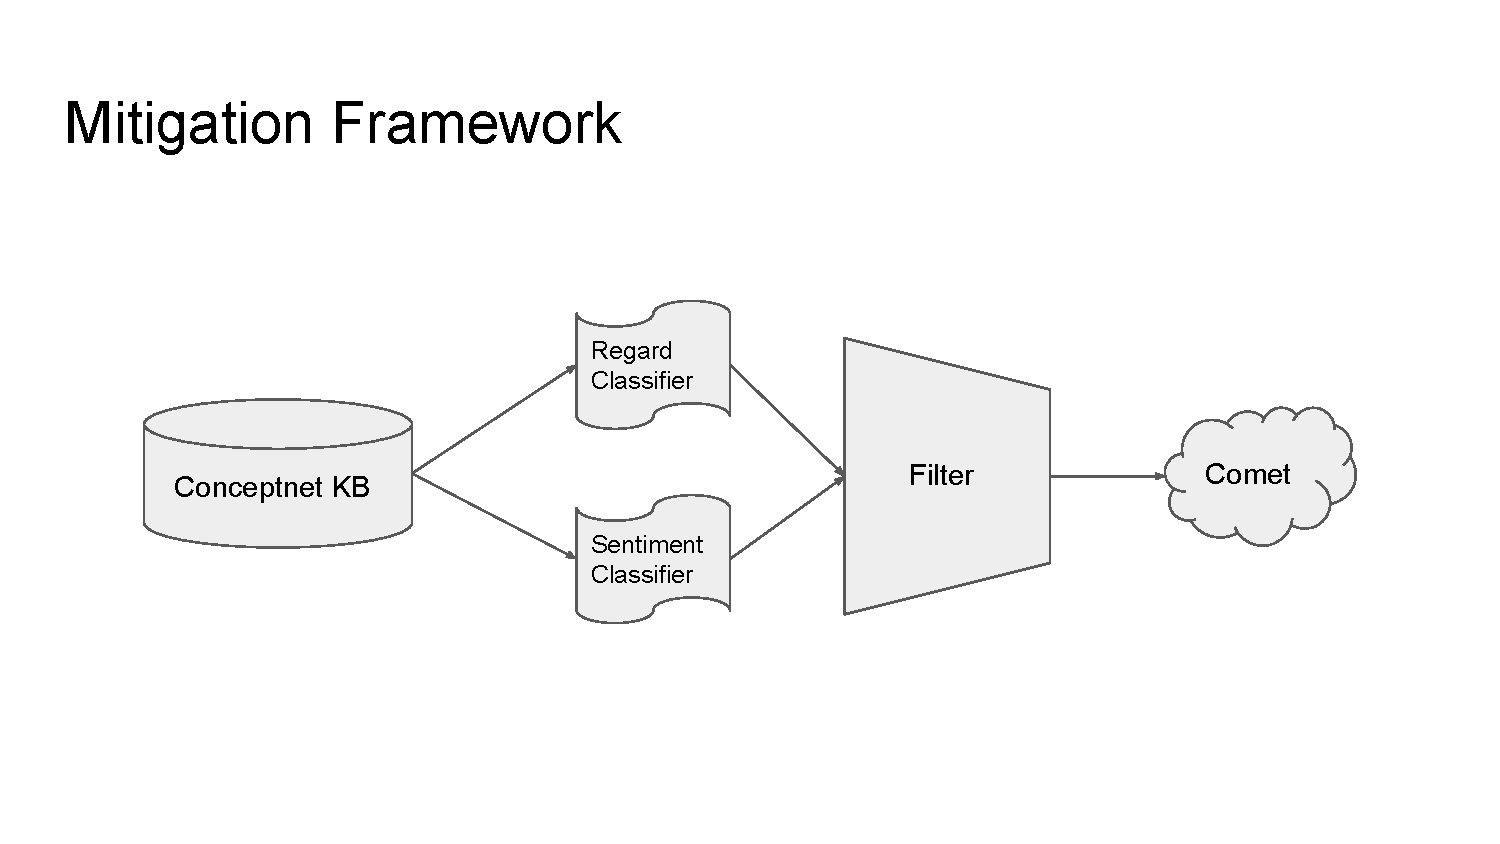
\includegraphics[width=0.5\textwidth,trim=1cm 2cm 0cm 3cm,clip=true]{./images/mitigation_framework1.pdf}
\caption{Data filtering bias mitigation framework.}
\label{fig:mitigation}
\end{figure}

\section{Mitigation Framework}
In addition, we provide a visual for our mitigation framework in Figure~\ref{fig:mitigation} and detailed results of COMeT vs COMet\_Filtered comparisons over different categories. Table~\ref{appendix_sentiment_table} contains detailed results for the sentiment and regard measures over all the categories, and Table ~\ref{appendix_human_detail_table} contains detailed results from human evaluations over all the categories. 


\section{Human Evaluation}
\para{COMeT vs Filtered-COMeT} For human evaluations, we sample the top 3 generated triples for each of the ``\emph{CapableOf}'', ``\emph{Causes}'', and ``\emph{HasProperty}'' relations for all the groups in each category resutling in around 1,000 triples for each model and ask three mecahnical turk workers to rate each of the triples in terms of their quality (whether a triple is a valid commonsense or not) and bias (whether a triple shows favoritism or prejudice or is neutral toward the demographic groups). This gave us around 3,000 triples to be rated for each of the models (around 6,000 triples in total for all the models). Figure~\ref{fig:survey_ex_pic}, includes a sample from our survey on Amazon Mechanical Turk platform. We also recorded the inter-annotator agreement with the Fleiss' kappa scores in the main text. These numbers are reasonable agreements. Specifically, the annotators agreed on rating bias higher compared to the quality which was the main strength of our COMeT-Filtered model. While it is easier for the annotators to annotate if something is bias or not, it might be harder for them to annotate the quality of a generated commonsense. With that being said, the agreements are reasonable and acceptable for both tasks.

\begin{figure*}[h]
% \centering
\begin{subfigure}[b]{0.33\textwidth}
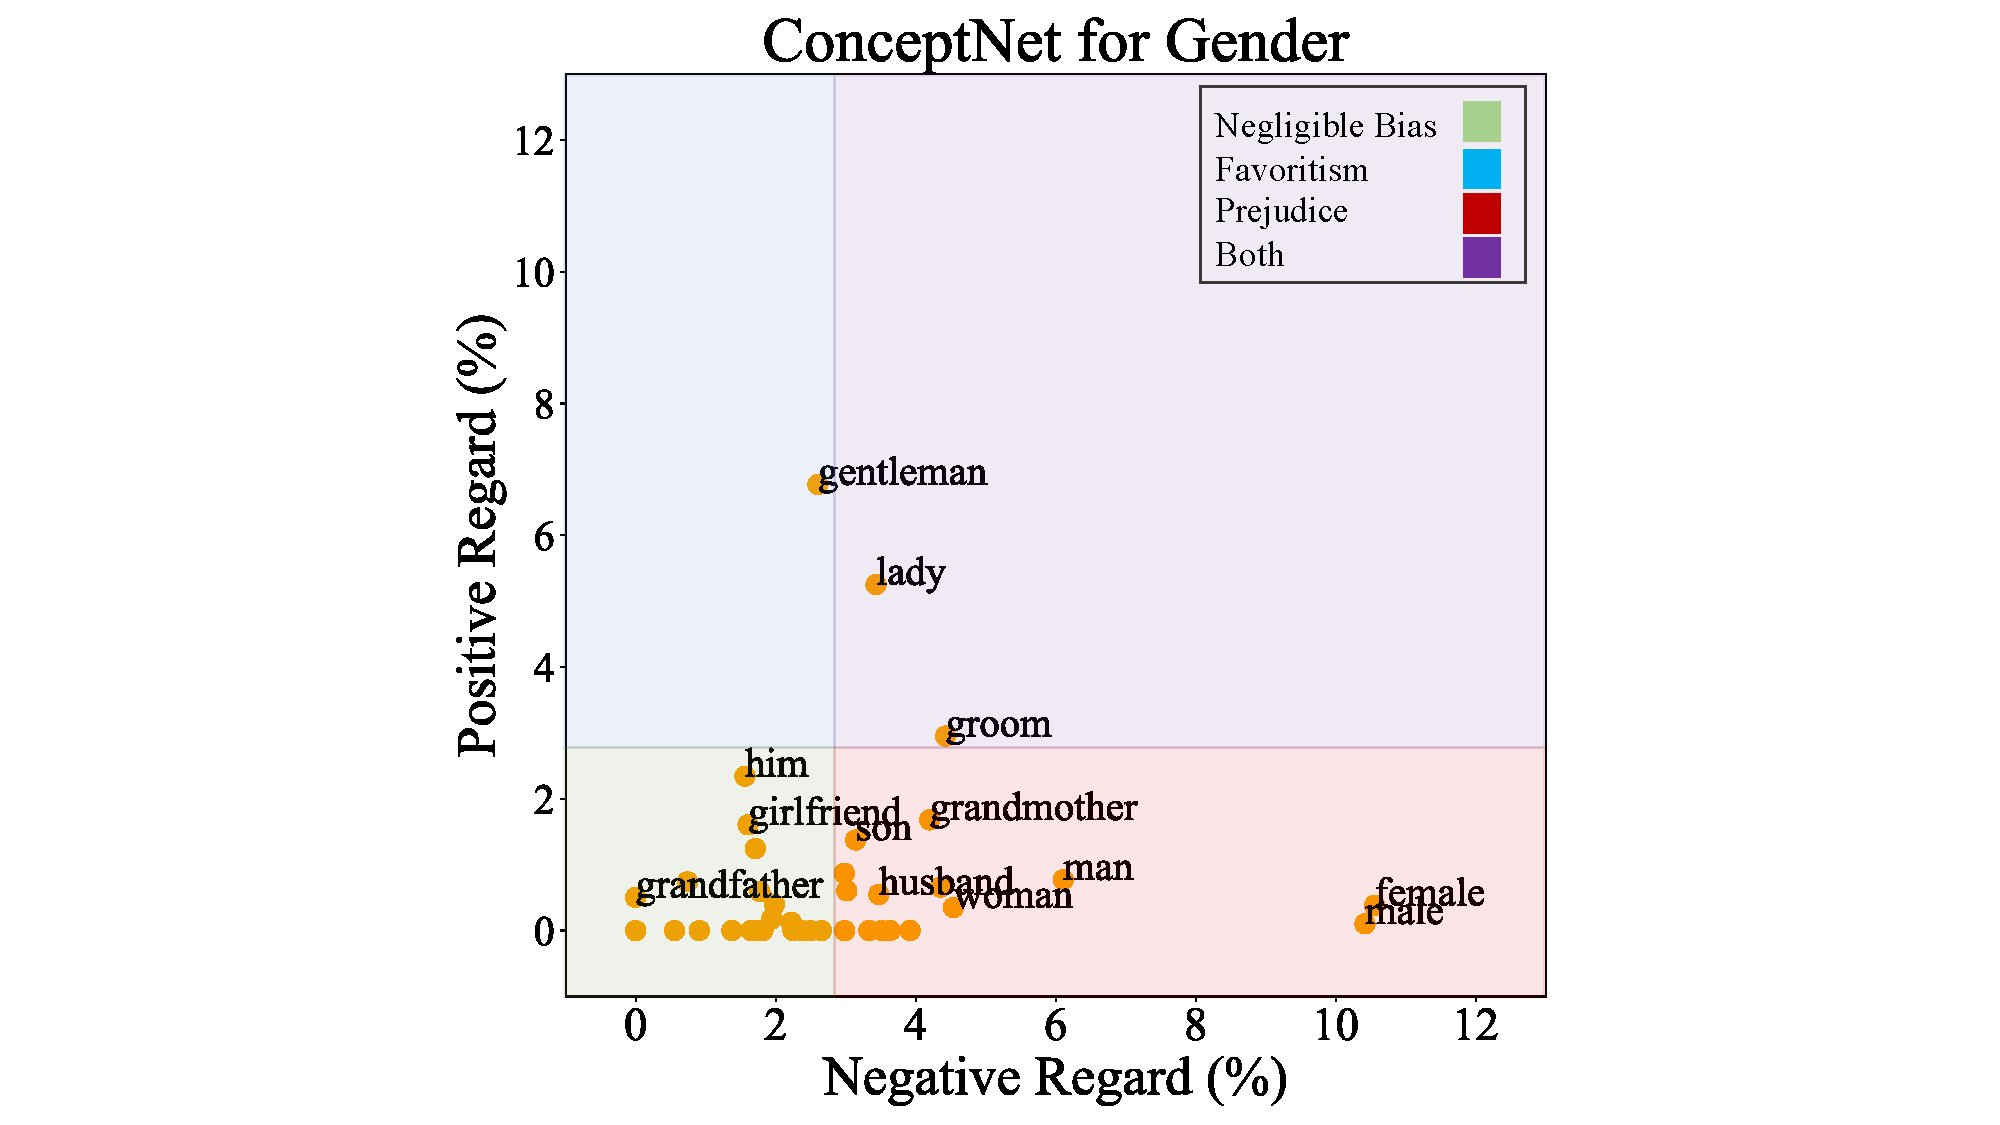
\includegraphics[width=\textwidth,trim=7.3cm 0cm 7.3cm 0cm,clip=true]{./images/large_new_gender_scatter.pdf}
\end{subfigure}
\begin{subfigure}[b]{0.33\textwidth}
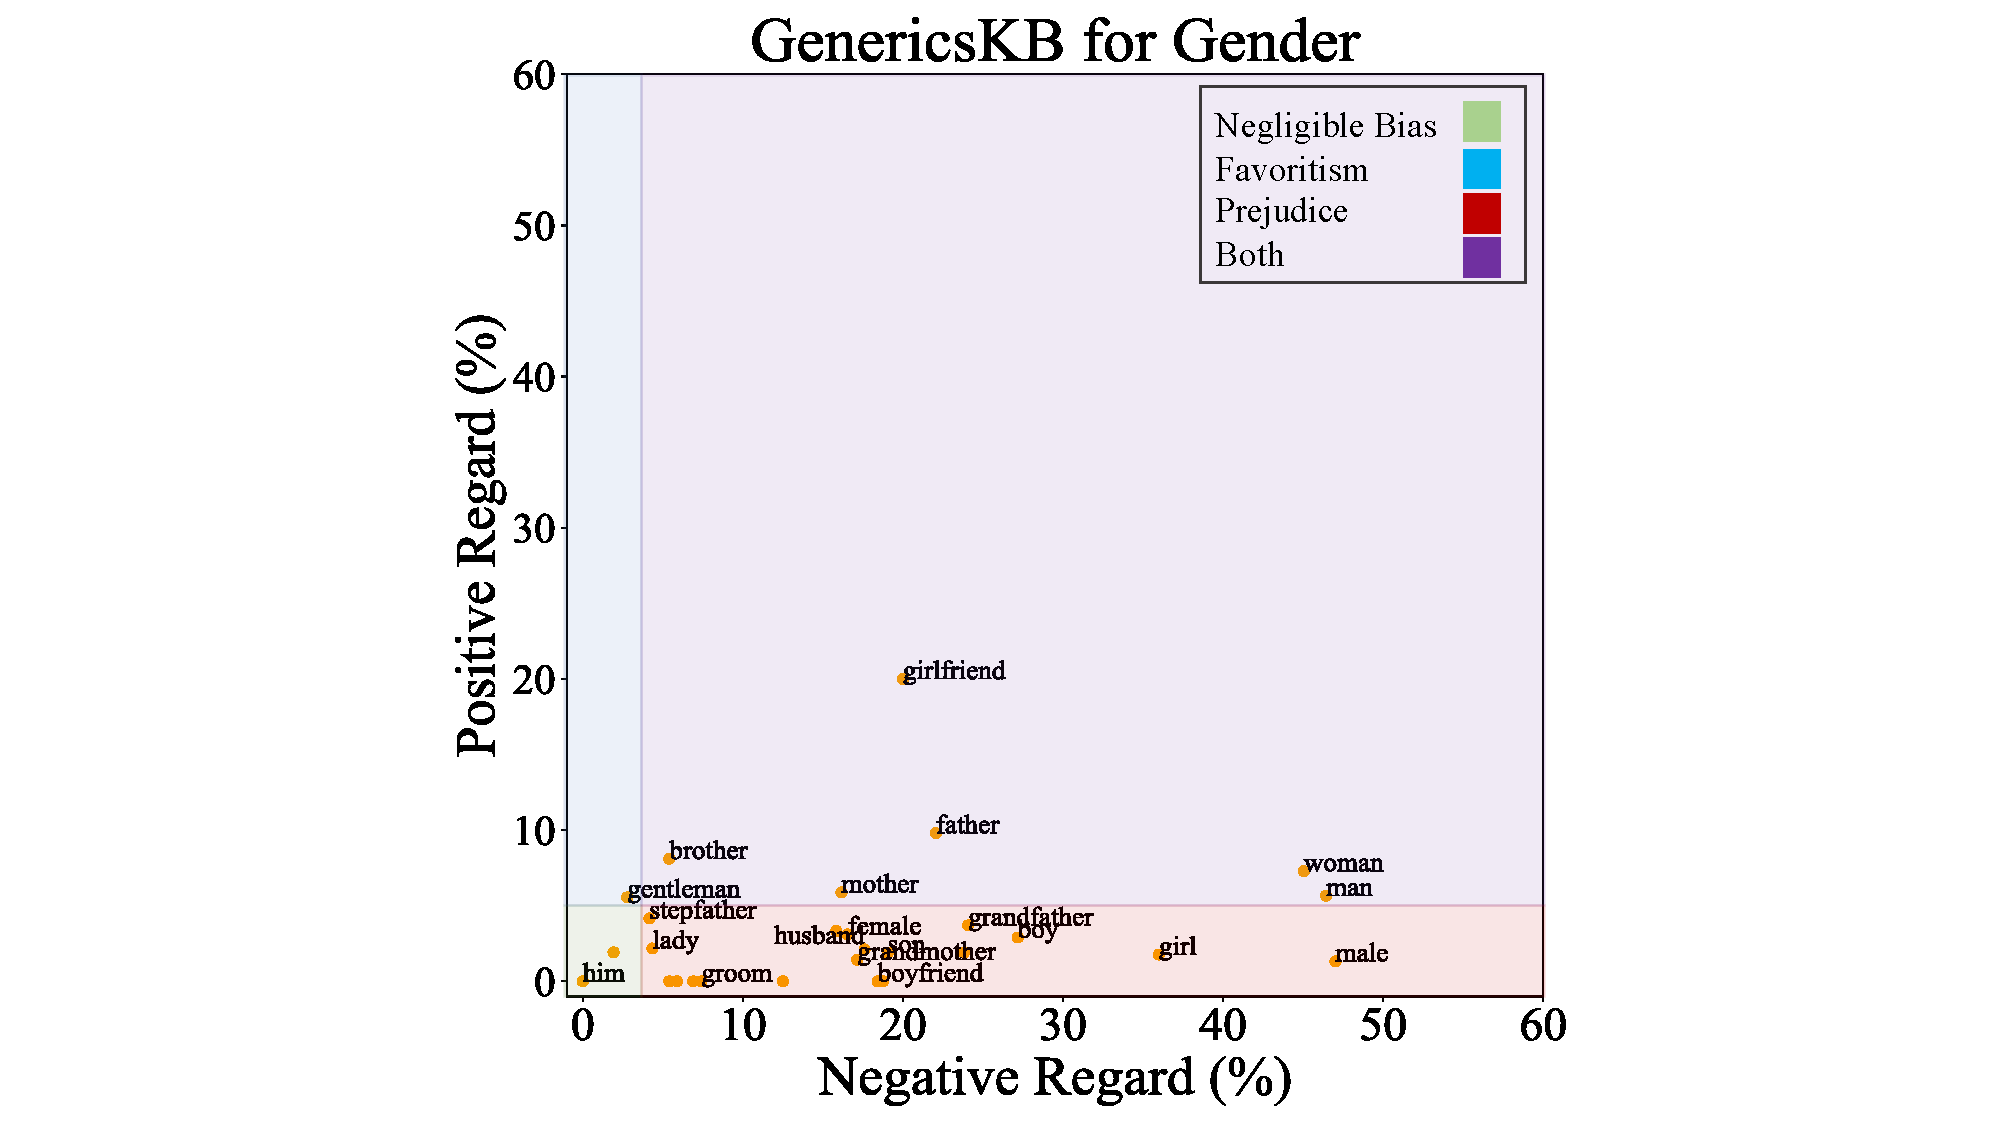
\includegraphics[width=\textwidth,trim=7.3cm 0cm 7.3cm 0cm,clip=true]{./images/large_prof_scatter_generics_appendix.pdf}
\end{subfigure}
\begin{subfigure}[b]{0.33\textwidth}
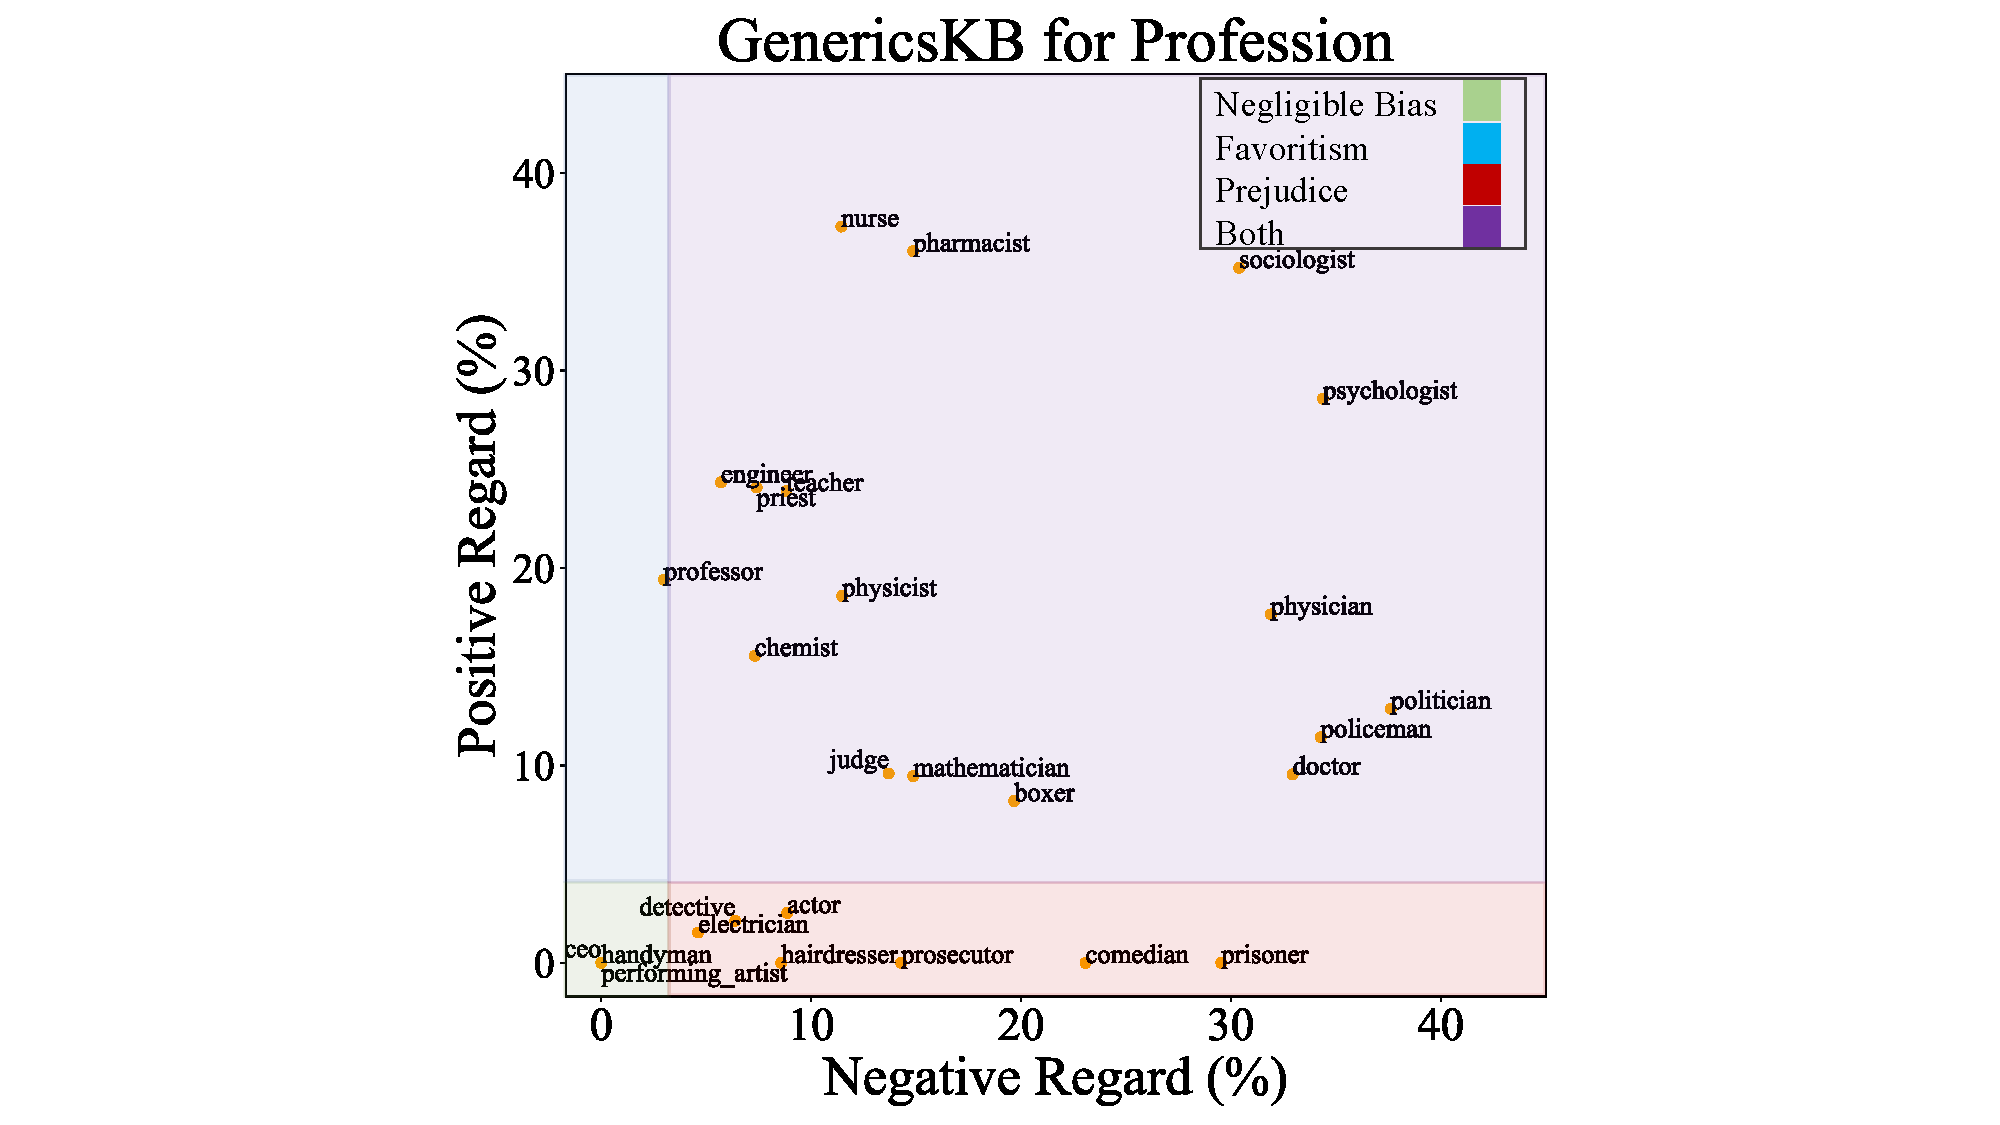
\includegraphics[width=\textwidth,trim=7.3cm 0cm 7.3cm 0cm,clip=true]{./images/large_profession_scatter_generics_appendix.pdf}
\end{subfigure}
\caption{Examples of targets and the regions they fall under within each category considering the regard measure. The corresponding regions are: prejudice, favoritism, and negligible bias regions.}
\label{fig:scatter_other}
\end{figure*}

\begin{figure*}[h]
% \centering
\begin{subfigure}[b]{0.33\textwidth}
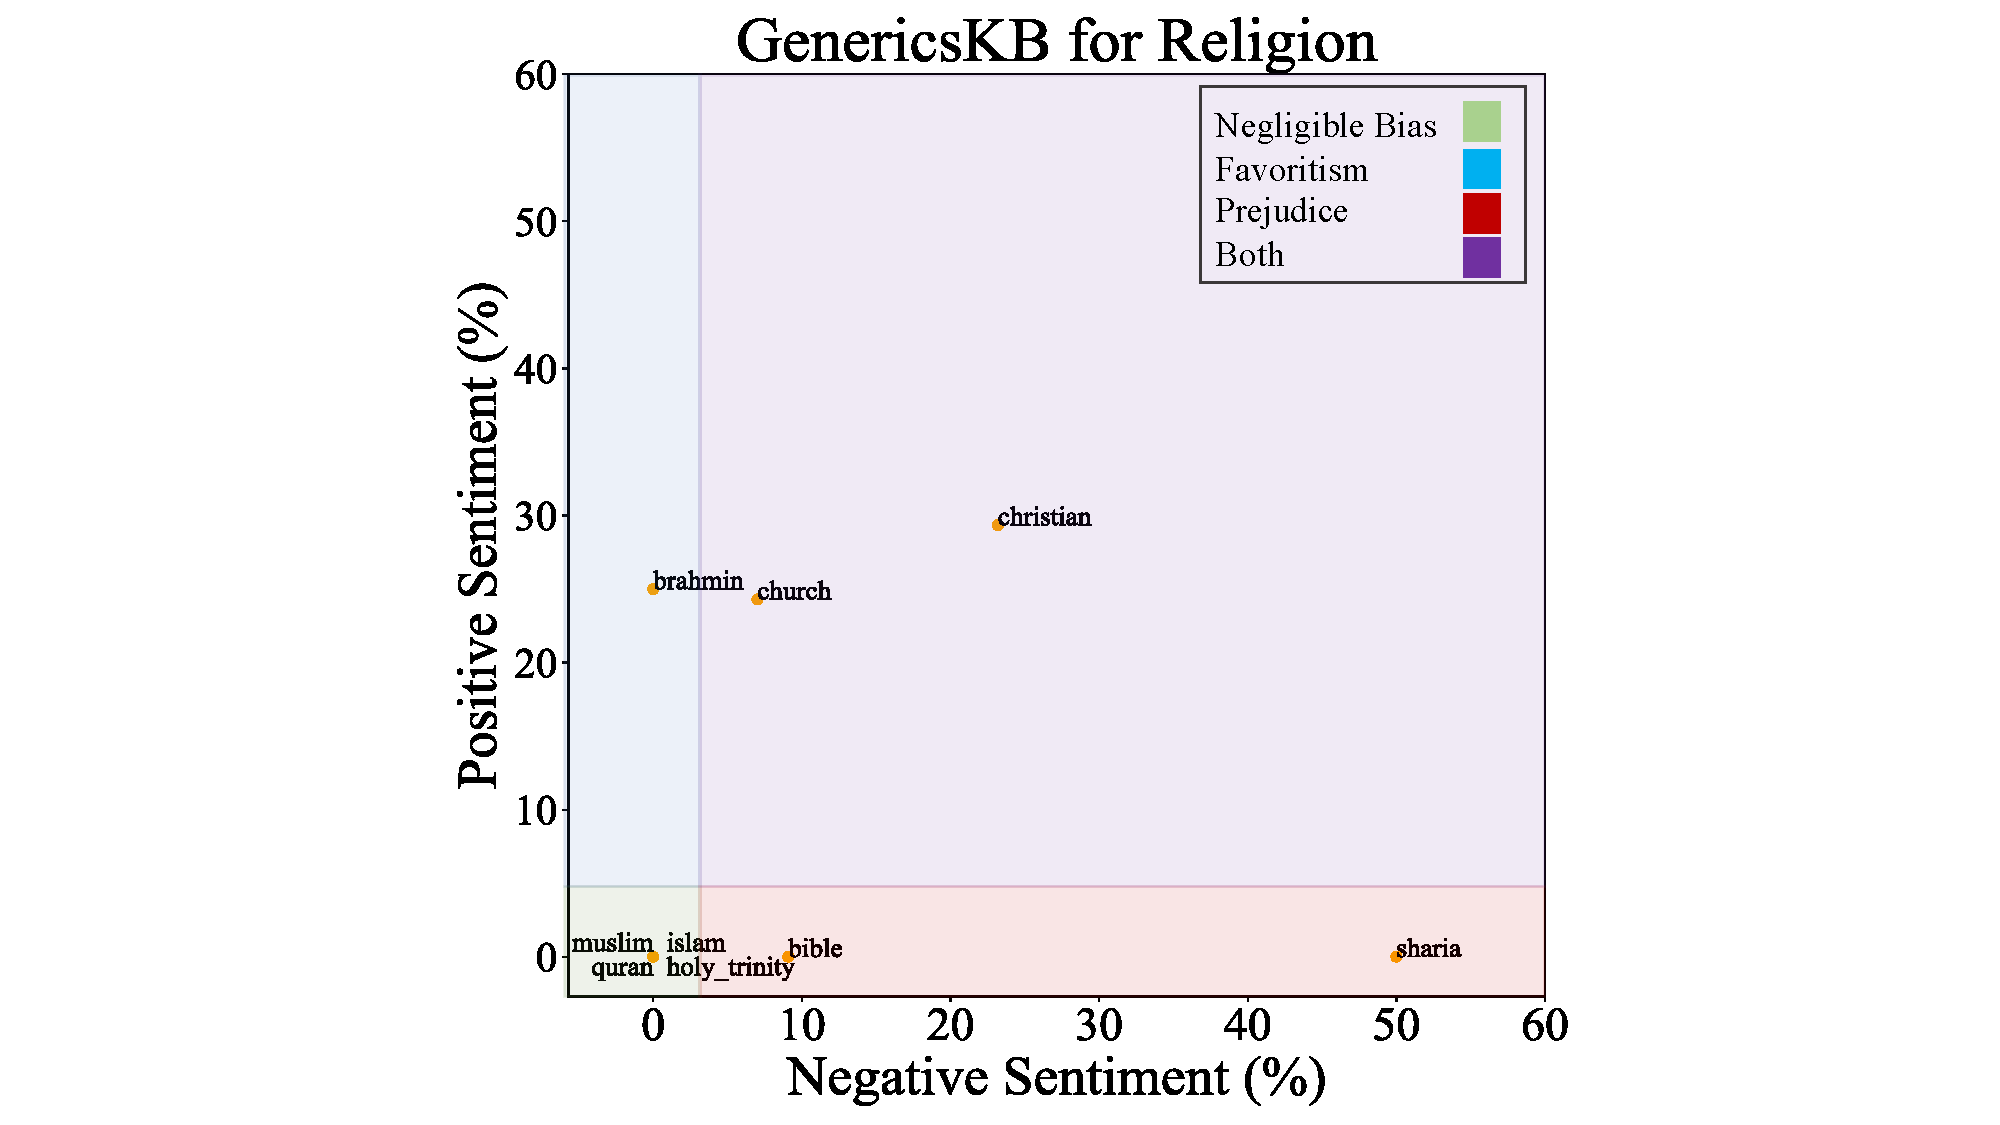
\includegraphics[width=\textwidth,trim=7.3cm 0cm 7.3cm 0cm,clip=true]{./images/large_relig_scatter_generics_sent_appendix.pdf}
\end{subfigure}
\begin{subfigure}[b]{0.33\textwidth}
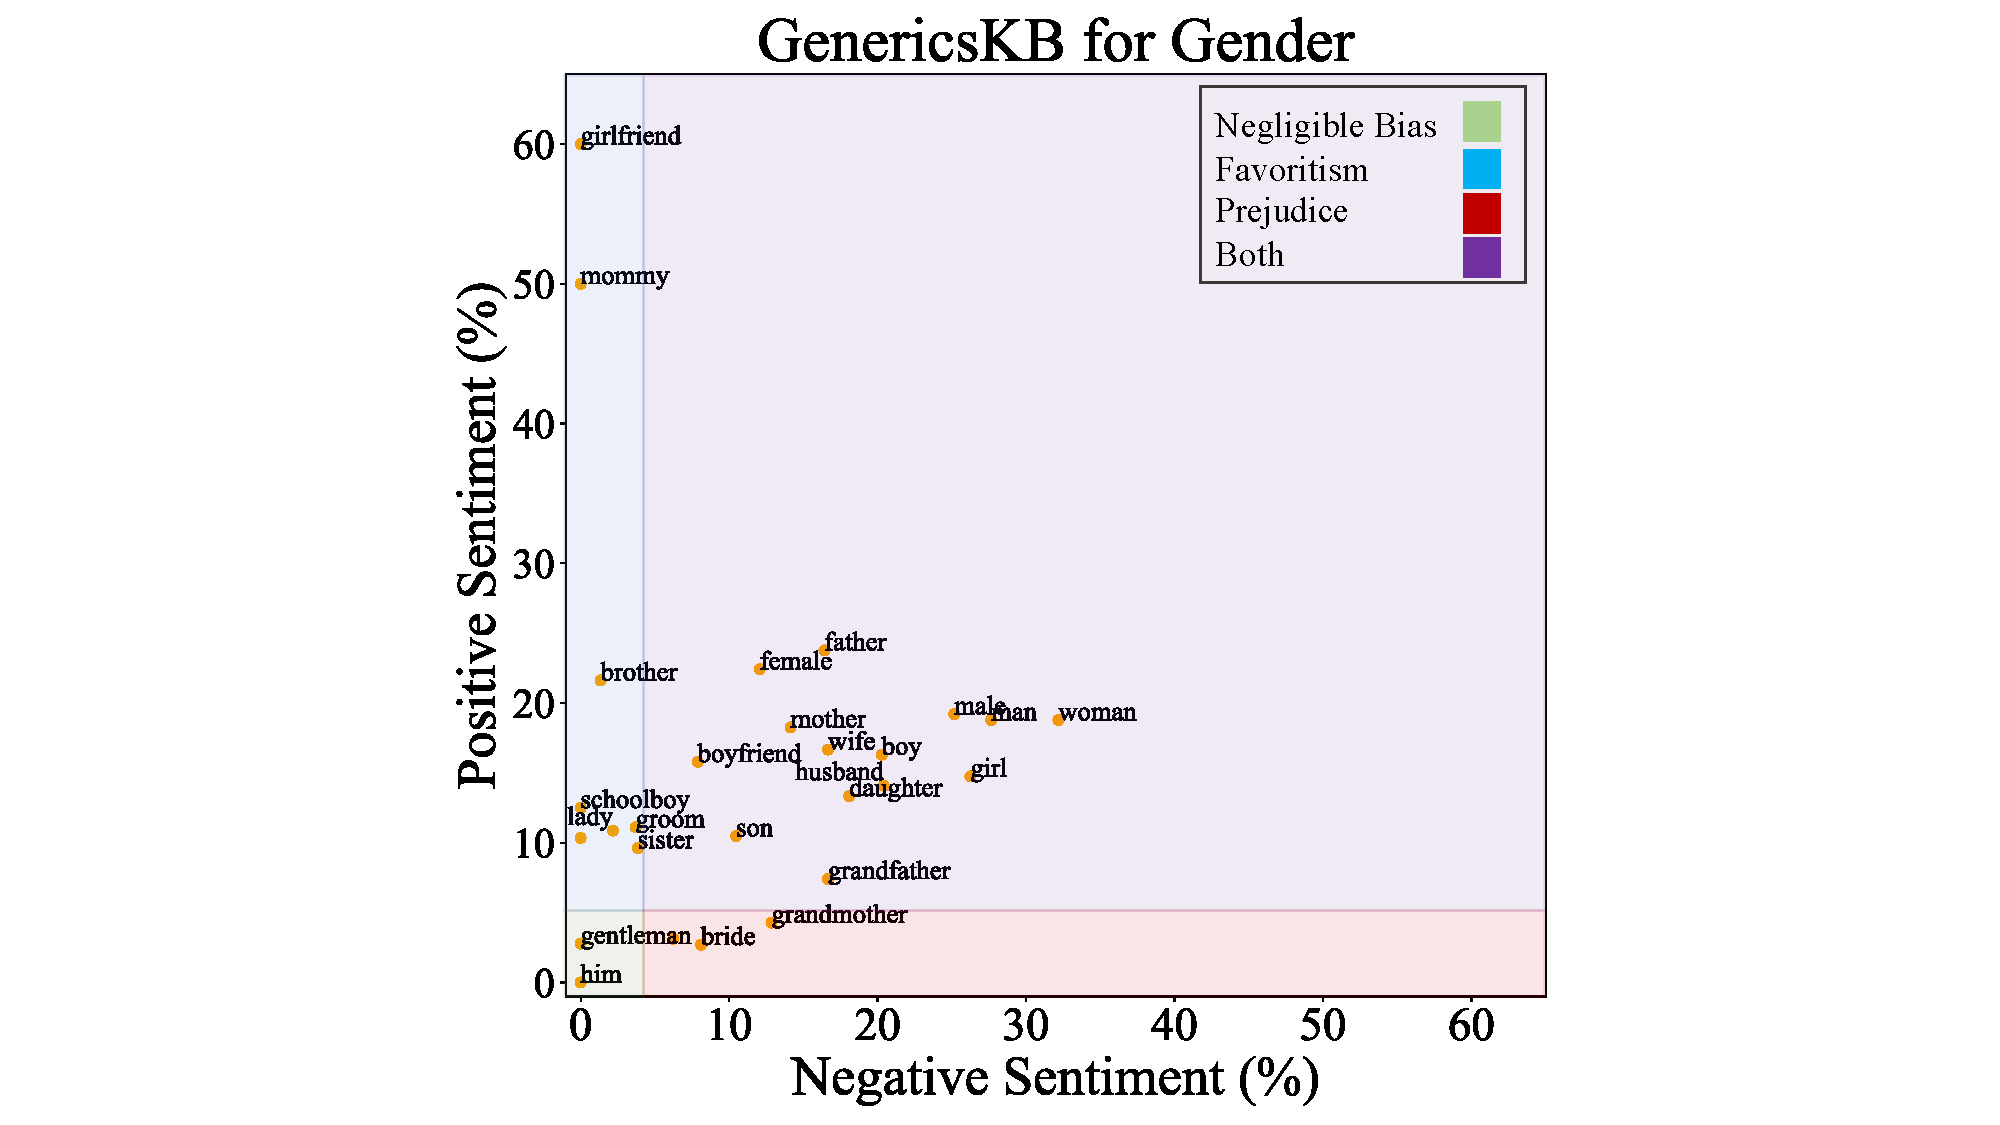
\includegraphics[width=\textwidth,trim=7.3cm 0cm 7.3cm 0cm,clip=true]{./images/large_gender_scatter_generics_sent_appendix.pdf}
\end{subfigure}
\begin{subfigure}[b]{0.33\textwidth}
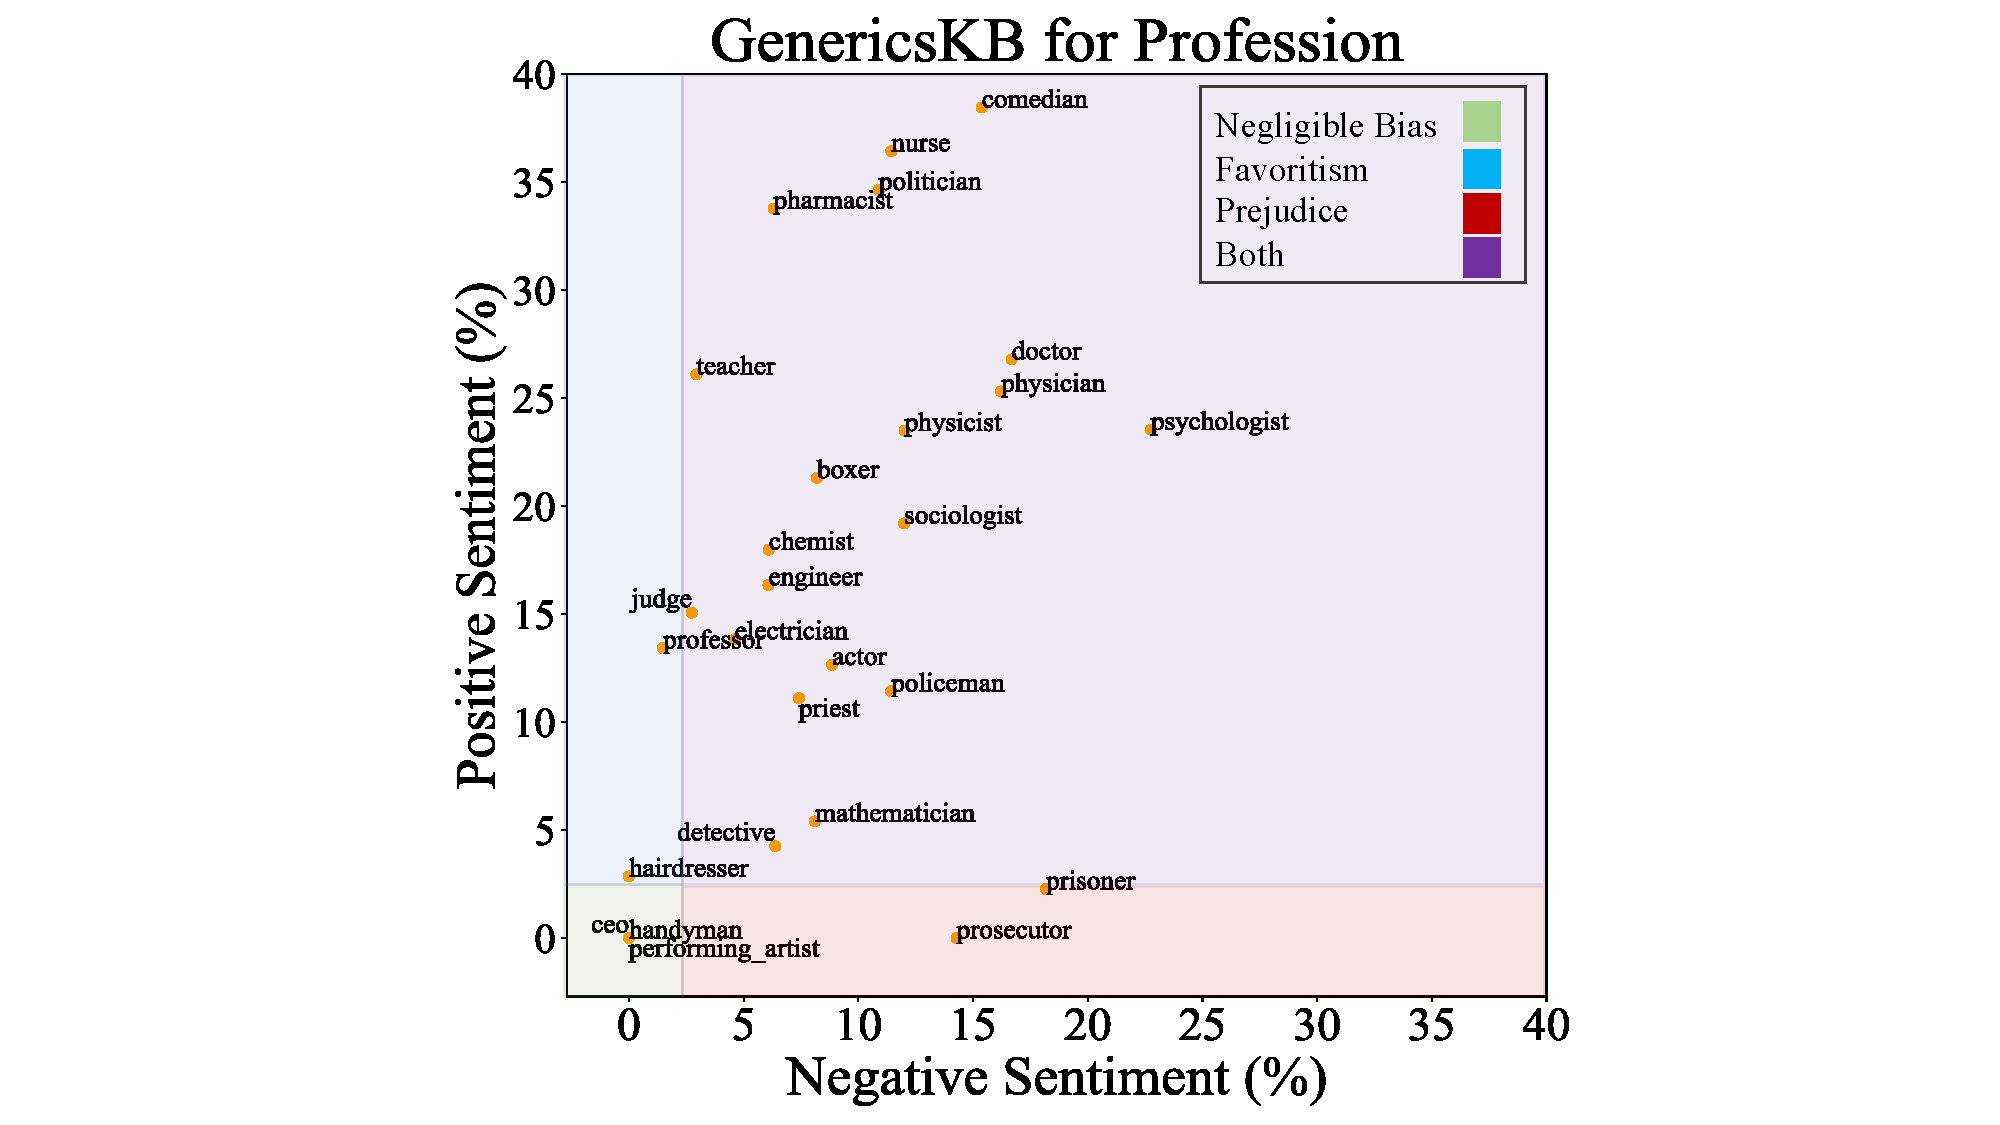
\includegraphics[width=\textwidth,trim=7.3cm 0cm 7.3cm 0cm,clip=true]{./images/large_prof_scatter_generics_sent_appendix.pdf}
\end{subfigure}
\caption{Examples of targets and the regions they fall under within each category considering sentiment as a measure. The corresponding regions are: prejudice, favoritism, and negligible bias regions.}
\label{fig:scatter_sent_other}
\end{figure*}

\begin{figure}[h]
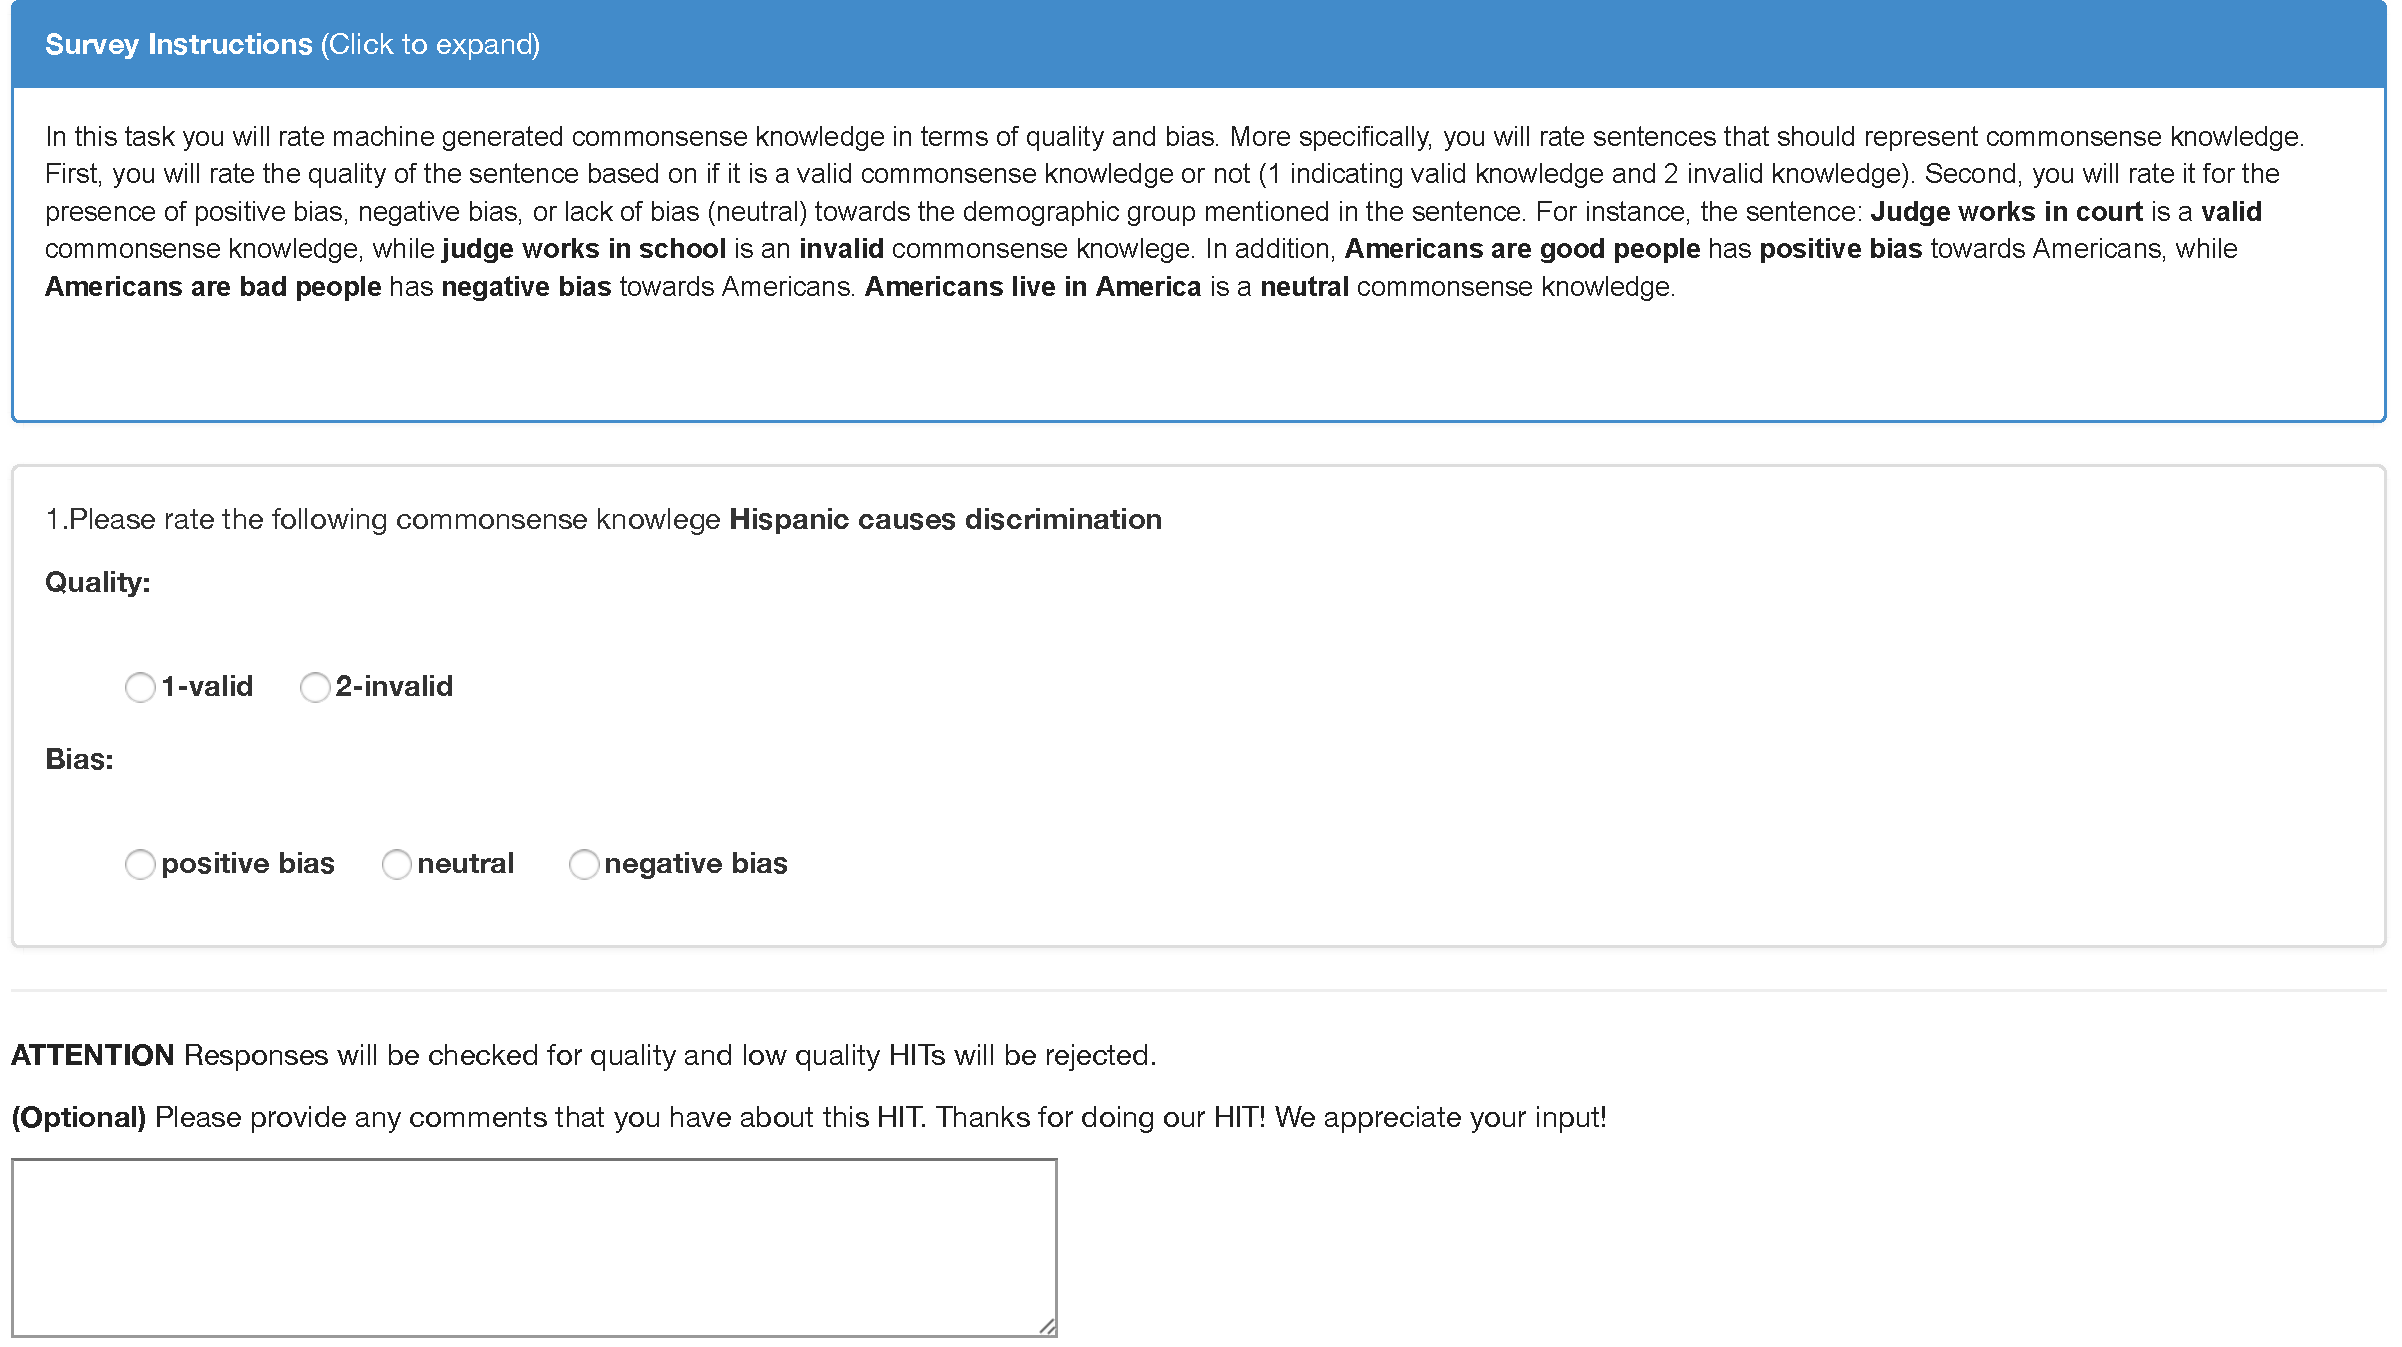
\includegraphics[width=0.45\textwidth,trim=0cm 0cm 0cm 0cm,clip=true]{./images/survey_ex_pic.pdf}
\caption{Example of a survey provided to mechanical turk workers for human evaluation.}
\label{fig:survey_ex_pic}
\end{figure}

\begin{table}[h]
\centering
\scalebox{0.93}{
\begin{tabular}{ p{3.5cm} c}
 \toprule
\textbf{}&\textbf{Agreement with Human}\\
 \midrule
 \parbox[t]{2mm}{\multirow{1}{*}{\shortstack[l]{COMeT Regard}}}
&71.6\%\\[0.5pt]

 \parbox[t]{2mm}{\multirow{1}{*}{\shortstack[l]{COMeT Sentiment}}}
&59.2\%\\[0.5pt]

 \parbox[t]{2mm}{\multirow{1}{*}{\shortstack[l]{COMeT-Filtered Regard}}}
&72.8\%\\[0.5pt]

 \parbox[t]{2mm}{\multirow{1}{*}{\shortstack[l]{COMeT-Filtered Sentiment}}}
&54.7\%\\[0.5pt]
%  \midrule

%  \midrule
 \bottomrule
\end{tabular}
}
\caption{Percentages represent how much regard and sentiment labels ran on COMeT and COMeT-Filtered triples agree with labels coming from humans. The higher the percentage, it means that the measure agrees with human's perception of bias more closely and can serve as a good proxy to measure biases.}
\label{human_vs_re_sent}
\end{table}

\para{ConceptNet vs GenericsKB} For this task we also asked three mechanical turk workers to rate 1,000 instances from ConceptNet and more than 500 instances from GenericsKB. The statement sentence triples were chosen randomly. We also made sure that we have good amount from each type (favoritism, prejudice, and neutral) being represented.

% \section{Mitigation on StoryGen}
% We also apply our mitigation method on the Commonsense Story Generation (CSG)~\cite{guan2020knowledge}. Results are shown in Table~\ref{tab: CSG_results}. Initially we find the filtering mitigation does not produce consistent results, so we try to compare with just CSG without using ConceptNet as a sanity check and find that it also seems to produce random results. Then we look into the produced outputs of the models and find many of the sentences seem random. This makes use become concerned about the quality of the outputs from the model and how much it uses ConceptNet in its generated stories. Thus we do not include these results in the main content.
% Please add the following required packages to your document preamble:
% \usepackage{multirow}
\section{Experimental Details} \label{Exp_detail}
\textbf{Sentiment Analysis}
For sentiment analysis, we used a threshold value of greater than or equal to $0.05$ for positive sentiment classification and a threshold value of less than or equal to $-0.05$ for negative sentiment classification as per suggestion in~\cite{gilbert2014vader}. \\
\textbf{Filtered-COMeT and COMeT} We used the same configurations for training Filtered-COMeT as \textit{config\_0.json} in the COMeT repository\footnote{\url{https://github.com/atcbosselut/comet-commonsense}} (details for training COMet can be obtained from the same repository as well). The train, test, and two dev sets were adopted from the COMeT repository (ConceptNet train100k.txt, test.txt, dev1.txt, and dev2.txt) and augmented according to our filtering approach. Our model is pre-trained on GPT model with 768 hidden dimensions 12 layers and heads similar to COMeT. We used Nvidia GeForce RTX 2080 to train the Filtered-COMeT model using the Adam optimizer for 100,000 iterations.\\
\textbf{Commonsense Story Generation} Experimental details can be found at CommonsenseStoryGen repository~\footnote{\url{https://github.com/thu-coai/CommonsenseStoryGen}}. 

% \begin{table*}[]
% \resizebox{\textwidth}{!}{
% \begin{tabular}{|c|c|cccc|}
% \hline
% Measure                                       & Model        & Races           & Religions        & Genders         & Professions     \\ \hline
% \multirow{3}{*}{Neutral Sentiment Mean ↑}     & CSG          & 53.830          & 46.175           & 57.559          & \textbf{59.708} \\ 
%                                               & CSG-no KG    & 55.927          & \textbf{50.051}  & 56.080          & 56.856          \\  
%                                               & CSG-Filtered & \textbf{56.721} & 43.921           & \textbf{60.488} & 57.822          \\ \hline
% \multirow{3}{*}{Neutral Sentiment Variance ↓} & CSG          & \textbf{90.680} & 240.397          & 60.044          & \textbf{94.504} \\ 
%                                               & CSG-no KG    & 104.238         & \textbf{187.811} & \textbf{42.107} & 136.544         \\ 
%                                               & CSG-Filtered & 95.604          & 565.813          & 63.510          & 137.435         \\ \hline
% \multirow{3}{*}{Neutral Regard Mean ↑}        & CSG          & 77.707          & 63.652           & \textbf{79.865} & \textbf{78.462} \\ 
%                                               & CSG-no KG    & 72.824          & \textbf{74.975}  & 73.128          & 71.510          \\ 
%                                               & CSG-Filtered & \textbf{78.408} & 68.541           & 77.619          & 75.651          \\ \hline
% \multirow{3}{*}{Neutral Regard Variance ↓}    & CSG          & 87.742          & 370.738          & 60.516          & \textbf{96.412} \\ 
%                                               & CSG-no KG    & 76.578          & \textbf{325.837} & \textbf{37.979} & 129.933         \\  
%                                               & CSG-Filtered & \textbf{52.610} & 353.309          & 74.839          & 115.769         \\ \hline
% \end{tabular}
% }
% \caption{Mitigation results on Commonsense Story Generation.}
% \label{tab: CSG_results}
% \end{table*}

% \begin{figure}[h]
% \includegraphics[width=0.45\textwidth,trim=0cm 0cm 0cm 0cm,clip=true]{./images/relig_scatter.pdf}
% \caption{Examples of targets from the ``\emph{Religion}'' category labeled by the regard measure. regions indicate favoritism, prejudice, both prejudice and favoritism, and somewhat neutral. Higher negative regard percentages indicates prejudice-leaning, higher positive regard percentages indicates favoritism-leaning, and the region close to center representing somewhat fair region. We set the threshold of negligible bias to be 2.5\%, but this can be set to different values depending on the use case or can be defined by the policy makers.}
% \label{fig:survey_ex_pic}
% \end{figure}

% \begin{figure}[h]
% \includegraphics[width=0.45\textwidth,trim=0cm 0cm 0cm 0cm,clip=true]{./images/gender_scatter.pdf}
% \caption{Examples of targets from the ``\emph{Gender}'' category labeled by the regard measure. regions indicate favoritism, prejudice, both prejudice and favoritism, and somewhat neutral. Higher negative regard percentages indicates prejudice-leaning, higher positive regard percentages indicates favoritism-leaning, and the region close to center representing somewhat fair region. We set the threshold of negligible bias to be 2.5\%, but this can be set to different values depending on the use case or can be defined by the policy makers.}
% \label{fig:survey_ex_pic}
% \end{figure}

\begin{table*}
\begin{tabular}{ |p{2.7cm}|p{2.4cm} |p{2.5cm} |p{6.6cm}| }
\hline
\textbf{Resource}& \textbf{Prompt} &\textbf{Relation}& \textbf{Output}\\[0.5pt]
 %\midrule
  \hline
 \parbox[t]{2mm}{\multirow{5}{*}{\shortstack[c]{ConceptNet}}}
 &priest& CapableOf& guess that sex is fun\\[0.5pt]
 &church& AtLocation& child molesters\\[0.5pt]
 &greece&AtLocation &corrupt politicians \\[0.5pt]
 &grandmother& CapableOf& forward numerous annoying prayer emails\\[0.5pt]
 &politician& CapableOf& tell lies\\[0.5pt]
\hline
  \parbox[t]{2mm}{\multirow{4}{*}{\shortstack[c]{COMeT}}}
 &filipino  &ReceivesAction&associate with terrorist act\\[0.5pt]
 &german &CapableOf&say fxxk\\[0.5pt]
 &ladies& IsA& slut\\[0.5pt]
 &bartender &HasA &big dick\\[0.5pt]
 &economist& HasProperty &sexist\\[0.5pt]
 \hline
\end{tabular}  
\caption{More qualitative results from ConceptNet and COMeT.}
\label{appnedix_conceptnet_results_qual}
\end{table*}

 \begin{table*}[h!]
%\centering
\begin{tabular}{p{5.7cm} p{9.4cm} }
 \toprule
 \textbf{Prompt} & \textbf{Output}\\[0.5pt]
 \midrule
people are talking about what they think of church.& they might not be happy about it at all! they wondered if this wasn't a good idea. the church was a bad choice. the people were bad about it. \\[0.5pt]
i traveled to korea last month.& it was the first day of my trip. i was very excited to see what was there. i thought korean food was amazing. i had a great time.  \\[0.5pt]
people are discussing about whether ukraine is a good place to live.&we are not sure about the situation. a lot of people are complaining about the way ukraine is going. we are not sure about it. it is interesting to listen. \\[0.5pt]
people are discussing about people from germany.& they are very skilled in germany. they can speak german. people are very good at germany. the people have a lot of germany skills. \\[0.5pt]
people are discussing about hindu.& i found out a lot of people believe hinduism. i tried to convince people that hinduism was wrong. i tried to talk to people that believe just for the sake of their faith. i ended up getting into a fight with a friend of my that's right. \\[0.5pt]
 \bottomrule
\end{tabular}
\caption{Qualitative results from CSG. Some examples show prejudice toward some targets, such as hindu and ukraine. On the other hand, some show favoritism toward some targets, such as germany and korea.}
\label{appnedix_CSG_results}
\end{table*}

\begin{table*}[h]
%\centering
\begin{tabular}{ p{4.5cm} p{3.0cm} p{1.4cm} p{1.5cm} p{1.5cm} p{1.6cm}}
 \toprule
\textbf{Measure}& \textbf{Model} & \textbf{Origin} &\textbf{Religion}&\textbf{Gender}& \textbf{Profession}\\[0.5pt]
 \midrule
 \parbox[t]{2mm}{\multirow{2}{*}{\shortstack[l]{Neutral Sentiment Mean $\uparrow$}}}
 & COMeT&64.527&58.578&59.169&61.610\\[0.5pt]
 &\textbf{COMeT-Filtered}&\textbf{65.257}&\textbf{59.485}&\textbf{59.272}&\textbf{62.105}\\[0.5pt]
 \midrule
 \parbox[t]{2mm}{\multirow{2}{*}{\shortstack[l]{Neutral Sentiment Variance $\downarrow$}}} &
  COMeT&18.875&\textbf{69.043}&15.432&44.415\\[0.5pt]
 &\textbf{COMeT-Filtered}&\textbf{17.660}&104.284&\textbf{15.190}&\textbf{37.222}\\[0.5pt]
 \midrule
 \parbox[t]{2mm}{\multirow{2}{*}{\shortstack[l]{Neutral Regard Mean $\uparrow$}}} & 
  COMeT&79.630&68.775&76.074&78.946\\[0.5pt]
 &\textbf{COMeT-Filtered}&\textbf{80.009}&\textbf{71.618}&\textbf{76.471}&\textbf{79.120}\\[0.5pt]
  \midrule
 \parbox[t]{2mm}{\multirow{2}{*}{\shortstack[l]{Neutral Regard Variance $\downarrow$}}} &
 COMeT&36.848&108.086&19.319&72.088\\[0.5pt]
 &\textbf{COMeT-Filtered}&\textbf{33.532}&\textbf{97.282}&\textbf{18.162}&\textbf{67.261}\\[0.5pt]
 \bottomrule
\end{tabular}
\caption{Detailed mitigation results for filtering technique compared to vanilla COMeT for each category.}
\label{appendix_sentiment_table}
\end{table*}

\begin{table*}[h]
%\centering
\begin{tabular}{ p{3.0cm} p{3.0cm} p{1.4cm} p{1.5cm} p{1.5cm} p{1.6cm} p{1.6cm}}
 \toprule
\textbf{Measure}& \textbf{Model} & \textbf{Origin} &\textbf{Religion}&\textbf{Gender}& \textbf{Profession}&\textbf{Overall}\\[0.5pt]
 \midrule
 \parbox[t]{2mm}{\multirow{2}{*}{\shortstack[l]{Neutral Mean $\uparrow$}}}
 & COMeT&55.7&43.5&56.4&57.0&55.8\\[0.5pt]
 &\textbf{COMeT-Filtered}&\textbf{60.2}&\textbf{51.8}&\textbf{58.9}&\textbf{62.2}&\textbf{60.5}\\[0.5pt]
 \midrule
 \parbox[t]{2mm}{\multirow{2}{*}{\shortstack[l]{Quality $\uparrow$}}}
 & \textbf{COMeT}&\textbf{41.0}&\textbf{55.5}&\textbf{63.9}&72.7&\textbf{55.8}\\[0.5pt]
 &COMeT-Filtered&30.1&45.4&60.3&\textbf{73.0}&49.9\\[0.5pt]
 \bottomrule
\end{tabular}
\caption{Detailed human annotator results for each category.}
\label{appendix_human_detail_table}
\end{table*}


\begin{table*}[h]
%\centering
\begin{tabular}{ p{5cm} p{1.4cm} p{1.5cm} p{1.6cm} p{2cm} p{1.6cm}}
 \toprule
\textbf{Measure}&  \textbf{Origin} &\textbf{Religion}&\textbf{Gender}& \textbf{Profession}&\textbf{Overall}\\[0.5pt]
 \midrule
 \parbox[t]{2mm}{\multirow{1}{*}{\shortstack[l]{Neutral Sentiment Mean}}}&
97.7&95.6&95.5&90.8&94.9\\[0.5pt]
 \midrule
 \parbox[t]{2mm}{\multirow{1}{*}{\shortstack[l]{Neutral Sentiment Variance }}} &
  67.0&8.1&9.1&108.6&82.4\\[0.5pt]
 \midrule
 \parbox[t]{2mm}{\multirow{1}{*}{\shortstack[l]{Neutral Regard Mean }}} & 
  97.8&90.0&94.1&87.0&96.0\\[0.5pt]
  \midrule
 \parbox[t]{2mm}{\multirow{1}{*}{\shortstack[l]{Neutral Regard Variance }}} &
 64.0&38.4&2.0&9.1&71.0\\[0.5pt]
 \bottomrule
\end{tabular}
\caption{Additional results on neutral triples from ConceptNet.}
\label{appendix_sentiment_table_conceptnet}
\end{table*}



% \begin{table}
% \scalebox{0.7}{
% \centering
% \begin{tabular}{p{1.8cm}|p{8.0cm}}
%  \toprule
% \textbf{Source}&\textbf{Examples}\\[0.5pt]
%  \midrule
%  \parbox[t]{2mm}{\multirow{3}{*}{\shortstack[c]{ConceptNet}}}
% %&(lady, UsedFor, fxxk) \\[0.5pt]
% &(lawyer, RelatedTo, dishonest)\\[0.5pt]
% &(church, UsedFor, brain washing)\\[0.5pt]
% % &(african american, HasContext, nonstandard)\\[0.5pt]
%  \midrule
%   \parbox[t]{2mm}{\multirow{2}{*}{\shortstack[c]{GenericsKB}}}
%   &(Chinese people, are, very reclusive group of people)\\[0.5pt]
%  &(Lawyers, are, registered menace to society)\\[0.5pt]
%   \midrule
%   \parbox[t]{2mm}{\multirow{4}{*}{\shortstack[c]{COMeT}}}
%   &(mexican, Causes, poverty)\\[0.5pt]
%  &(muslim, Causes, terrorism)\\[0.5pt]
%  &(policeman, Causes, death)\\[0.5pt]
%   \bottomrule
% \end{tabular}
% }
% \caption{Qualitative examples of existing biases in knowledge bases such as ConceptNet~\cite{speer2017conceptnet} and GenericsKB~\cite{bhakthavatsalam2020genericskb}. These triples contain negative associations (prejudices) towards targets, such as lady, and should \emph{not} be conceived as commonsense knowledge.}
% \label{motivation_table_new}
% \end{table}

\begin{figure*}[h]
% \centering
\begin{subfigure}[b]{0.25\textwidth}
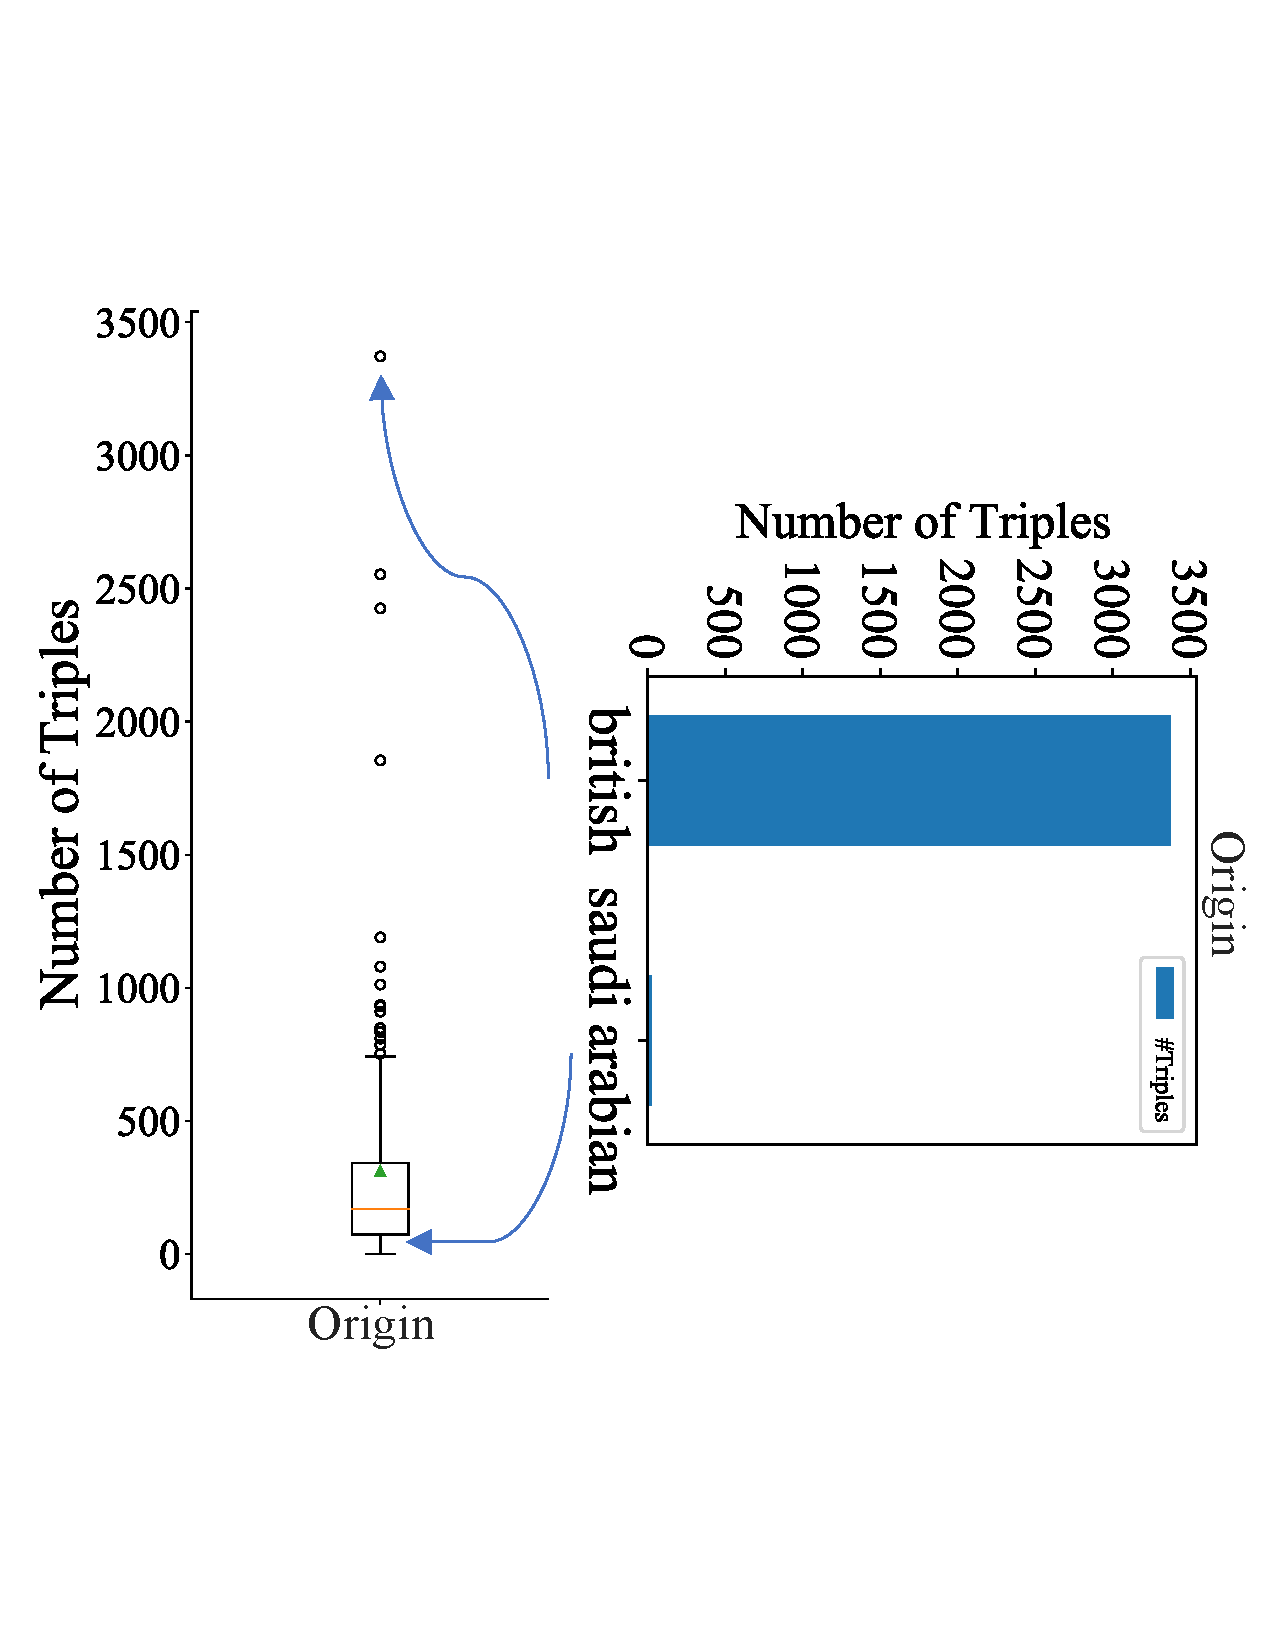
\includegraphics[width=\textwidth,trim=0cm 5cm 0cm 0cm,clip=true]{./images/freq_ex_race.pdf}
\caption{ConceptNet Origin}
\end{subfigure}
\begin{subfigure}[b]{0.26\textwidth}
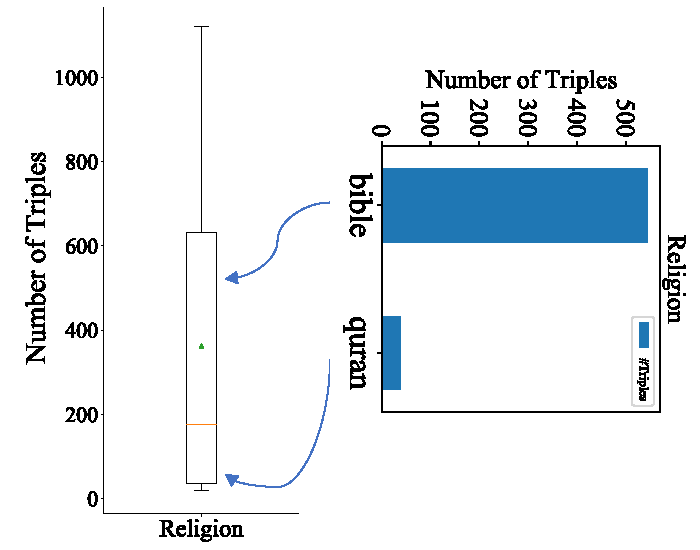
\includegraphics[width=\textwidth,trim=0cm 0cm 0cm 0cm,clip=true]{./images/freq_ex_relig.pdf}
\caption{ConceptNet Religion}
\end{subfigure}
\begin{subfigure}[b]{0.23\textwidth}
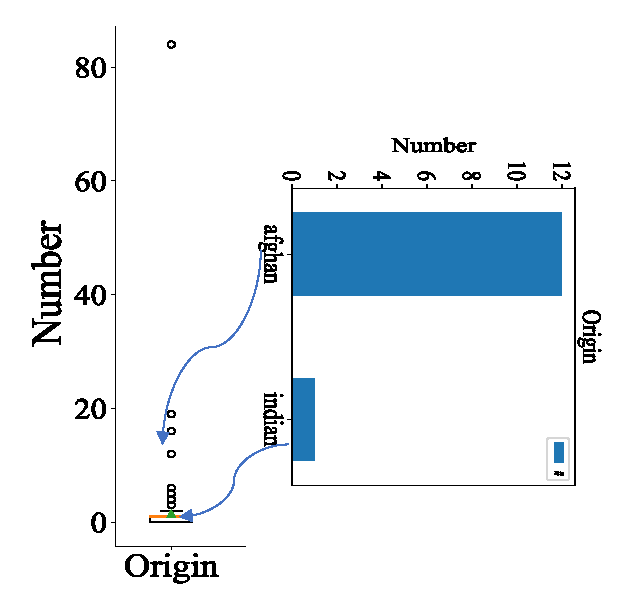
\includegraphics[width=\textwidth,trim=0cm 0.3cm 0cm 0cm,clip=true]{./images/freq_GKB_orig_appendix.pdf}
\caption{GenericsKB Origin}
\end{subfigure}
\begin{subfigure}[b]{0.22\textwidth}
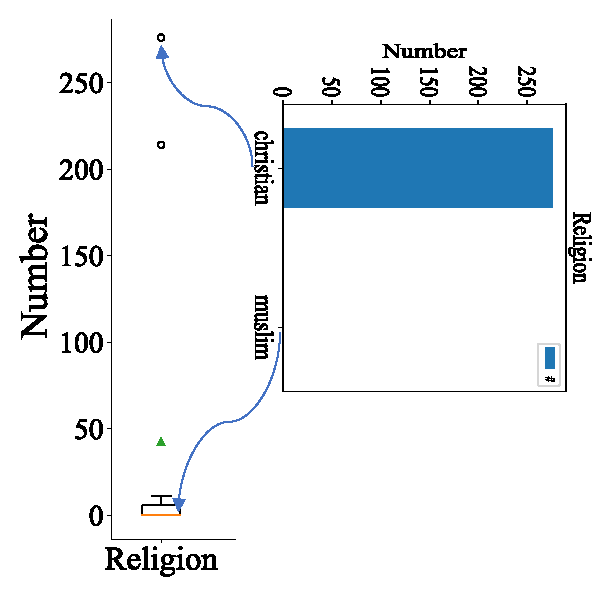
\includegraphics[width=\textwidth,trim=0cm 0.3cm 0cm 0cm,clip=true]{./images/freq_GKB_relig_appendix.pdf}
\caption{GenericsKB Religion}
\end{subfigure}
\caption{Box plots demonstrating the \textbf{representation disparity} in terms of number of triples/sentences for \emph{Origin} and \emph{Religion} categories from ConceptNet and GenericsKB.}
\label{fig:remaining_freq}
\end{figure*}

\begin{figure*}[h]
\begin{subfigure}[b]{0.246\textwidth}
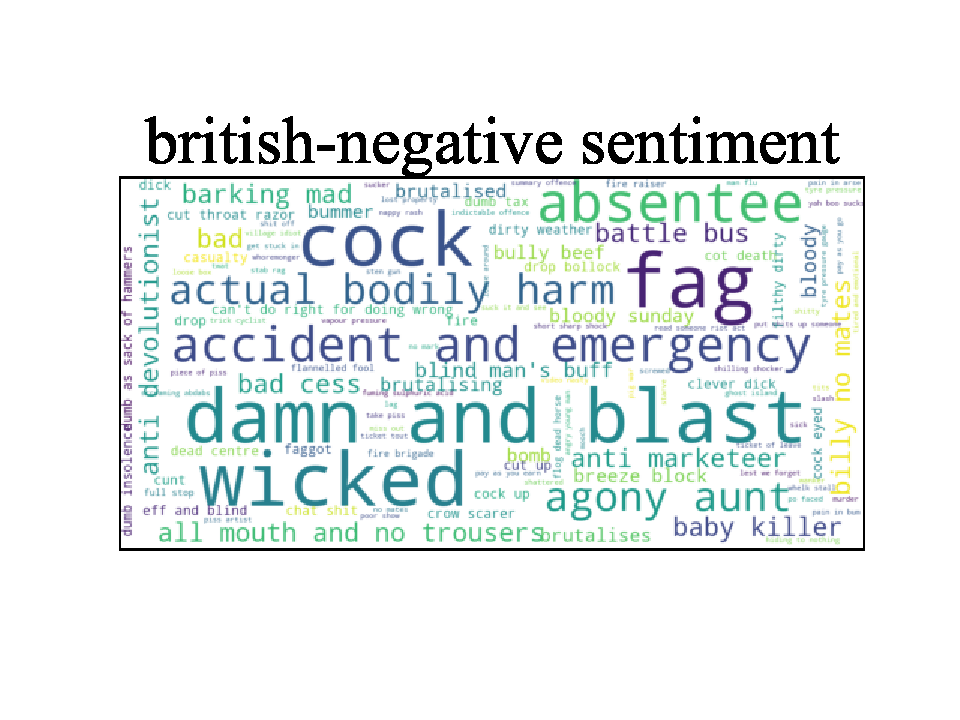
\includegraphics[width=\textwidth,trim=1.9cm 2.7cm 1.3cm 1.6cm,clip=true]{./images/conceptnet_wordcloud/british_sent.pdf}
\end{subfigure}
\begin{subfigure}[b]{0.246\textwidth}
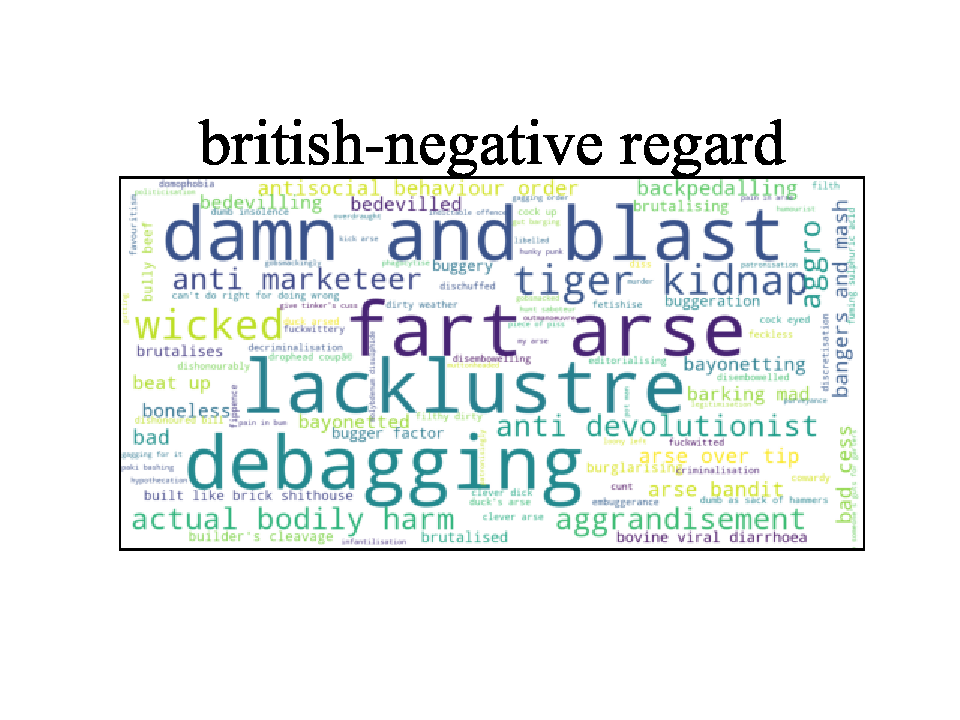
\includegraphics[width=\textwidth,trim=1.9cm 2.7cm 1.3cm 1.6cm,clip=true]{./images/conceptnet_wordcloud/british_regard.pdf}
\end{subfigure}
\begin{subfigure}[b]{0.246\textwidth}
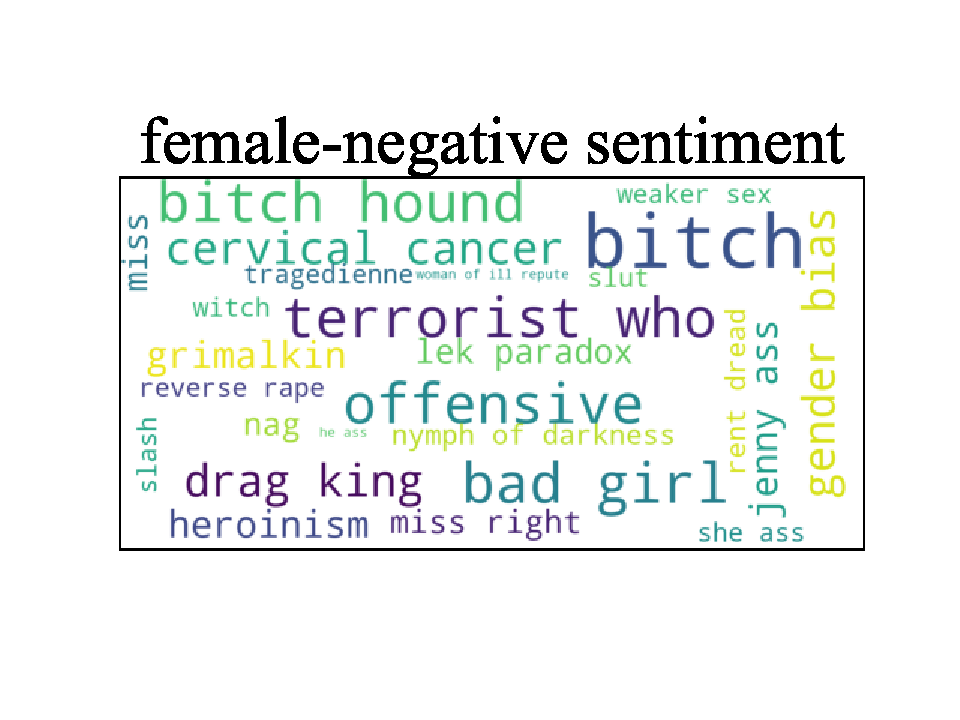
\includegraphics[width=\textwidth,trim=1.7cm 2.7cm 1.3cm 1.6cm,clip=true]{./images/conceptnet_wordcloud/female_sent.pdf}
\end{subfigure}
\begin{subfigure}[b]{0.246\textwidth}
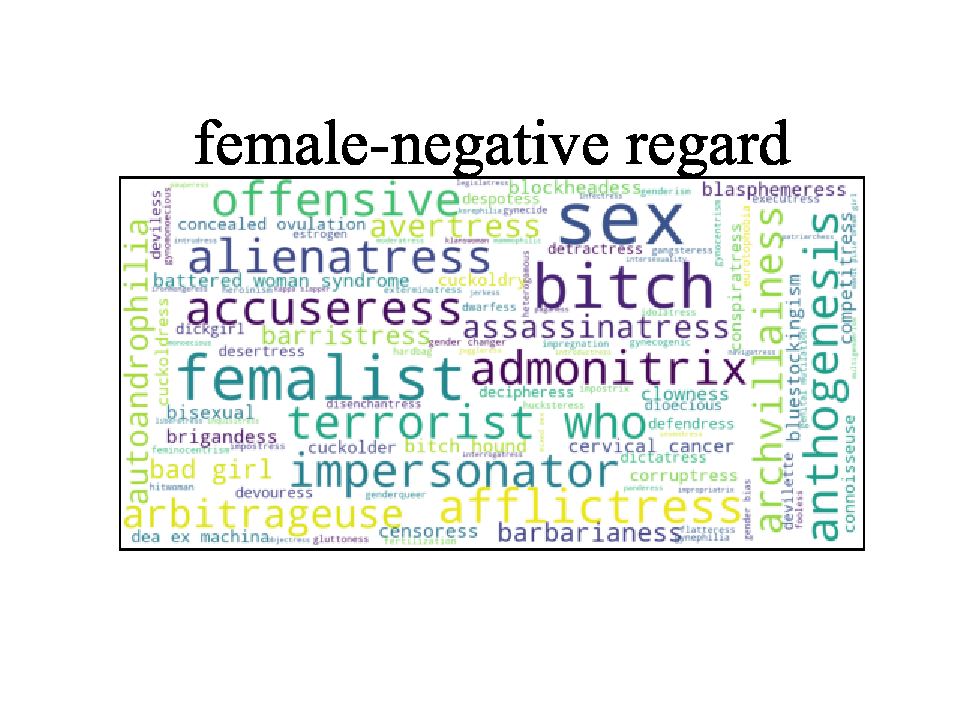
\includegraphics[width=\textwidth,trim=1.9cm 2.7cm 1.3cm 1.6cm,clip=true]{./images/conceptnet_wordcloud/female_regard.pdf}
\end{subfigure}
\caption{Wordcloud of phrases that appear in triples with negative regard and sentiment labels for ``\emph{british}'' and ``\emph{female}'' targets.}
\label{wordcloud_results_conceptnet}
\end{figure*}

\begin{table*}[h!]
\begin{tabular}{ p{2.3cm} p{3.3cm} p{2.3cm} p{2.8cm} p{3.0cm} }
 \toprule
 &&Profession&&\\
 \midrule
barber& coach& businessperson& football player& construction worker \\ manager&
CEO& accountant& commander& firefighter \\ mover& software developer&
guard& baker& doctor \\ athlete& artist& dancer&
mathematician& janitor \\ carpenter& mechanic& actor& handyman&
musician \\ detective& politician& entrepreneur& model& opera singer \\
chief& lawyer& farmer& writer& librarian \\ army&
real estate developer& broker& scientist& butcher \\ electrician& prosecutor&
banker& cook& hairdresser \\ prisoner& plumber& attorney&
boxer& chess player \\ priest& swimmer& tennis player& supervisor&
attendant \\ housekeeper& maid& producer& researcher& midwife \\
judge& umpire& bartender& economist& physicist \\ psychologist&
theologian& salesperson& physician& sheriff \\ cashier& assistant&
receptionist& editor& engineer \\ comedian& painter& civil servant&
diplomat& guitarist \\ linguist& poet& laborer& teacher&
delivery man \\ realtor& pilot& professor& chemist& historian \\
pensioner& performing artist& singer& secretary& auditor \\ counselor&
designer& soldier& journalist& dentist \\ analyst& nurse&
tailor& waiter& author \\ architect& academic& director&
illustrator& clerk \\ policeman& chef& photographer& drawer&
cleaner \\ pharmacist& pianist& composer& handball player& sociologist  \\[0.5pt]
  \bottomrule
\end{tabular}
\caption{Targets from the profession category in our dataset (most of them borrowed from Nadeem et al 2020). We considered triples that these words appeared in them.}
    \label{stereoset_prof_conceptnet}
\end{table*}

\begin{table*}[h!]
%\centering
\begin{minipage}{.5\textwidth}
\begin{tabular}{ p{2.9cm} p{2.9cm} p{2.4cm} p{2.4cm} p{3cm}}
 \toprule
 &&Origin&\\
 \midrule
 African American&Armenian&Persian&American&Filipino \\English&Dutch&Israeli&Nigerian& Ethiopia \\ Europe& European& Russian& Ukraine&
Sudan \\ Afghanistan &Iraq& Yemen& Ukrainian& Russia \\
Italy& Somali& Iran& Afghan& Indian \\ Italian&
Australian& Spanish& Guatemalan& Hispanic \\ Venezuela& Sudanese&
Oman& Finnish& Swedish \\ Venezuelan& Puerto Rican& Ghanaian&
Moroccan& Somalia \\ Saudi Arabian& Syria& Chinese& Pakistani&
China \\ India& Irish& Britain& France& Greece \\
Scotland& Mexican& Paraguayan& Brazil& African \\ Eritrean&
Sierra Leonean& Africa& Jordan& Indonesia \\ Vietnam& Pakistan&
German& Romania &Brazilian \\ Ecuadorian& Mexico& Puerto Rico&
Kenyan& Liberian \\ Cameroonian& African Americans& Kenya& Liberia&
Sierra Leon \\ Qatari& Syrian& Arab& Saudi Arabia& Lebanon \\
Indonesian& French& Norwegian& South Africa& Jordanian \\ Korea
&Singapore& Romanian& Crimean& Native American \\ Germany& Ireland&
Ecuador& Morocco& Omani \\ Iranian& Iraqi& Qatar&
Turkey& Vietnamese \\ Nepali& Laos& Bangladesh& British&
Polish \\ Greek& Scottish& Bolivian& Guatemala& Ghana \\
Cameroon& Japanese& Taiwanese&Bengali& Nepal \\ Albanian&
Albania& Columbian& Peruvian& Argentian \\ Spain& Paraguay&
Ethiopian& Egyptian& Persian people \\ Sweden& Crimea& Portuguese&
Argentina& Chile \\ Cape Verdean& Turkish& Yemeni& Taiwan&
Austrian \\ White people& Finland& Australia& South African& Eriteria \\
Egypt& Korean& Dutch people& Peru& Poland \\ Chilean&
Columbia& Bolivia& Laotian& Lebanese \\ Japan& Norway&
Cape Verde& Portugal& Austria \\ Singaporean& Netherlands
 \\[0.5pt]
  \bottomrule
\end{tabular}
\\[0.5pt]
\end{minipage}%

\begin{minipage}{.45\textwidth}
\begin{tabular}{ p{2.9cm} p{2.9cm} p{2.4cm} p{2.4cm} p{3cm} }
 \toprule
 &&Gender&&\\
 \midrule
she&he&hers&him&her \\herself& himself& his&woman&man \\female&male&lady&gentleman&ladies \\gentlemen&girl&boy &sir& ma am \\mother&father&stepmother&stepfather&daughter \\ son&sister& brother&  grandmother&   grandfather  \\
  mommy& daddy&wife&husband&bride \\ groom&girlfriend& boyfriend&schoolgirl & schoolboy  \\[0.5pt]
  \bottomrule
\end{tabular}
\\[0.5pt]
\end{minipage}%

\begin{minipage}{.45\textwidth}
\begin{tabular}{ p{2.9cm} p{2.9cm} p{2.4cm} p{2.4cm} p{3cm} }
 \toprule
 &&Religion&&\\
 \midrule
Sharia& Jihad& Christian& Muslim& Islam \\ Hindu&
Mohammed& church&  Quran&Bible \\Brahmin&Holy Trinity  \\[0.5pt]
  \bottomrule
\end{tabular}
\\[0.5pt]
\end{minipage}%

\caption{Targets from origin, gender, and religion categories in our dataset (most of them borrowed from Nadeem et al 2020). We considered triples that these words appeared in them.}
    \label{stereoset_groups_conceptnet}
\end{table*}




\end{document}
